
\documentclass[
                                          %
   12pt,                                % Schriftgroesse 12pt
   a4paper,                             % Layout fuer Din A4
   twoside,                             % Layout fuer beidseitigen Druck
   headinclude,                         % Kopfzeile wird Seiten-Layouts mit beruecksichtigt
   headsepline,                         % horizontale Linie unter Kolumnentitel
   plainheadsepline,                    % horizontale Linie auch beim plain-Style
   BCOR18mm,                            % Korrektur fuer die Bindung
   DIV14,                               % DIV-Wert fuer die Erstellung des Satzspiegels, siehe scrguide
   parskip=half,                        % Absatzabstand statt Absatzeinzug
   bibliography=totoc,                  % Literaturverz. wird ins Inhaltsverzeichnis eingetragen
   captions=tableheading,               % korrekte Abstaende bei TabellenUEBERschriften
%   openany,                            % Kapitel k�nnen auf geraden und ungeraden Seiten beginnen
   listof=totoc,                         % Abbildungs- und Tabellenverzeichnis in Inhaltsverz.
%   pointlessnumbers,                   % Kapitelnummern immer ohne Punkt
%   fleqn,                              % fleqn: Glgen links (statt mittig)
%  draft                               % Keine Bilder in der Anzeige, overfull hboxes werden angezeigt
%   chapterprefix,                      % x. Kapitel �ber Kapitel�berschrift schreiben
     ]{scrbook}[2001/07/30]             % scrbook-Version mind. 2.8j von 2001/07/30

%makeindex Studienarbeit.nlo -s nomencl.ist -o Studienarbeit.nls
\usepackage{ngerman}                    % neue Rechtschreibung
\usepackage[english]{babel}          % falls man in Englisch schreiben will
%\selectlanguage{german}
\selectlanguage{english}               % falls man in Englisch schreiben will
\usepackage{bibgerm}                    % Dt. Bibliothek 

\usepackage[latin1]{inputenc}           % Input-Encodung: latin1 fuer Unix
\usepackage[T1]{fontenc}                % T1-kodierte Schriften, korrekte Trennmuster fuer Worte mit Umlauten
\usepackage{ae}                         % F�r PDF-Erstellung
%\usepackage[hang]{caption2}             % mehrzeilige Captions ausrichten
%\usepackage{pifont}                     % f�r Zahlen im Kreis mit \ding{202} Google: symbols-a4.ps
\usepackage{graphicx}                   % zum Einbinden von Grafiken
\usepackage{float}                      % u.a. genaue Plazierung von Gleitobjekten mit H
\usepackage{tabularx}
\usepackage{amsmath}
\usepackage{amsfonts}
\usepackage{dsfont}
\usepackage{scrhack}
%  \newshadetheorem{definition}{Definition}
%  \newshadetheorem{folgerung}{Folgerung}
%  \newshadetheorem{thm}{Theorem}
  
%\usepackage{draftwatermark}
  
%\DeclareMathOperator{\grad}{grad}

%------------------Anfang Nummerierung Anhang-----------------
 \renewcommand\appendix{\par 
   \setcounter{section}{0}% 
   \setcounter{subsection}{0}% 
   \setcounter{figure}{0}%
   \renewcommand\thesection{\Alph{section}}% 
   \renewcommand\thefigure{\Alph{section}.\arabic{figure}}
   \renewcommand\theequation{\Alph{section}.\arabic{equation}}} 
%------------------Ende Nummerierung Anhang-----------------
%\usepackage{tocbasic}
\usepackage{wrapfig}
\usepackage{longtable}
%\usepackage{subfigure}
\usepackage{subfigure}
%\usepacka{gemes=falsre
%   colorlinks,linkcolor={black},citecolor={black},urlcolor={red},
%   pdfstartview={FitV},unicode,breaklinks=false]{hyperref}
%\usepackage{natbib}
% fuer Stichwortverzeichnis
%\usepackage{makeidx}
%\makeindex
%\renewcommand{\indexname}{Stichwortverzeichnis}
                                        % falls der Index nicht "`Index"' heissen soll
%\addcontentsline{toc}{section}{Stichwortverzeichnis}
                                        % falls das Stichwortverzeichnis im Inhaltsverzeichnis auftauchen soll


%\usepackage[ansinew]{inputenc}
                                        % Input-Encodung: ansinew fuer Windows

%\usepackage[centertags]{amsmath}
                                        % AMS-Mathematik, centertags zentriert Nummer bei split
%\usepackage{latexsym}
                                        % verschiedene Symbole
%\usepackage{textcomp}
                                        % verschiedene Symbole
\usepackage{pstricks}
%\usepackage{pst-all}
%                                        % PostScript Macros
\usepackage{psfrag}
\usepackage{pst-node}
\usepackage{psfrag}

%\usepackage{pstricks-add}  								% Standard PSTricks Paket
%\usepackage{pst-3dplot}								% 3D Plots mit PSTricks 
							% zus�tzliche PSTRicks Funktionalit�t
%\usepackage{rotating}	
%%%%%%%%%%%%%%%%%%%%%%%%%%%%%%%%%%%%%%%%%%%%%%%%%%%%%%
% M A K R O S   U N D   D E F I N I T I O N E N
%%%%%%%%%%%%%%%%%%%%%%%%%%%%%%%%%%%%%%%%%%%%%%%%%%%%%%

%%%%%%%%%%%%%%%%%%%% Symbole %%%%%%%%%%%%%%%%%%%%%%%%%


%%%%%%%%%%%%%%%%%%%%%%% PSTricks %%%%%%%%%%%%%%%%%%%%%%%%%%

%% Zur�cksetzen aller ver�nderten Werte
\newcommand{\psreset}{%
\psset{unit      = 1mm,
       xunit     = 1mm,
       yunit     = 1mm,
       linewidth = 1pt,
       linestyle = solid,
       linecolor = black,
       fillstyle = solid,
       fillcolor = white,
       Beta      = 0,
       Alpha     = 0}}

% Textgr��e
\newcommand{\textscale}{1}
% Liniendicken f�r Zeichnungen
\newlength{\lwFine}   \pssetlength{\lwFine}{0.1mm} % = 0.14mm
\newlength{\lwfine}   \pssetlength{\lwfine}{0.2mm} % = 0.14mm
\newlength{\lwnormal} \pssetlength{\lwnormal}{0.3mm} % = 0.21mm
\newlength{\lwthick}  \pssetlength{\lwthick}{0.5mm}
\newlength{\lwThick}  \pssetlength{\lwThick}{0.75mm} % = 0.64mm%

% verschiedene style Definitionen
\newpsstyle{normal}{arrowsize=1pt 3,arrowlength=2,arrowinset=0, linewidth=\lwnormal}%
\newpsstyle{koordpfeil}{arrowsize=2 0,arrowlength=2.5,arrowinset=0}%
%\newpsstyle{kdpfeil}{arrowsize=1.5 0,arrowlength=1.875,arrowinset=0,linewidth=\lwfine}%
\newpsstyle{masspfeil}{linewidth=\lwfine, arrowsize=2 0,arrowlength=2.5,arrowinset=0}%
%\newpsstyle{dottedline}{linestyle=dotted,dotsep=2pt}

\newpsstyle{PSGraphDash}{plotstyle=line,linewidth=0.8pt,linestyle=dashed,dash=4pt 4pt}
\newpsstyle{PSGraphSolidDot}{plotstyle=line,linewidth=0.8pt,linestyle=solid,showpoints=true}
\newpsstyle{PSGraphDot}{plotstyle=line,linewidth=1.2pt,linestyle=dotted,dotsep=2pt}
\newpsstyle{PSGraphDashDot}{plotstyle=line,linewidth=0.8pt,linestyle=dashed,dash=4pt 2pt 0.6pt 2pt}
\newpsstyle{PSGraphSolid}{plotstyle=line,linewidth=0.8pt,linestyle=solid}
\newpsstyle{PSGraphDashDotDot}{plotstyle=line,linewidth=0.8pt,linestyle=dashed,dash=4pt 2pt 0.6pt 2pt 0.6pt 2pt}
\newpsstyle{PSGraphPoint}{plotstyle=dots,dotstyle=*,dotsize=1.5}
% Schraffuren
\newpsstyle{hatchedu}{fillstyle=hlines,hatchwidth=\lwfine}
\newpsstyle{hatchedd}{fillstyle=vlines,hatchwidth=\lwfine}

%%%%%%%%%%%%%%%%%%%%%%%%% FARBEN %%%%%%%%%%%%%%%%%%%%%%%%%%%%%%%%%

\definecolor{LightBlue}{rgb}{0.68,0.85,0.9}
\definecolor{pink}{rgb}{1.0,0.066,0.9294}
\definecolor{darkgreen}{rgb}{0.251,0.678,0.188}
\definecolor{oker}{rgb}{1.0,0.686,0.3098}
\newgray{lgray}{0.65}
\newgray{llgray}{0.88}

\renewcommand{\rmdefault}{phv} % Arial
\renewcommand{\sfdefault}{phv} % Arial
% Integralzeichen f�r CAUCHY-Hauptwert und finite part nach HADAMARD
\def\Xint#1{\mathchoice
{\XXint\displaystyle\textstyle{#1}}%
{\XXint\textstyle\scriptstyle{#1}}%
{\XXint\scriptstyle\scriptscriptstyle{#1}}%
{\XXint\scriptscriptstyle\scriptscriptstyle{#1}}%
\!\int}
\def\XXint#1#2#3{{\setbox0=\hbox{$#1{#2#3}{\int}$}
\vcenter{\hbox{$#2#3$}}\kern-.5\wd0}}
\def\ddashint{\Xint=}
\def\dashint{\Xint-}
%\usepackage{lscape}
                                        % Seite im Querformat bei Erhalt der Kopfzeile
%\usepackage{verbatim}
                                        % Quellcode einbinden (\verbatiminput)
%\usepackage{multicol}
    \usepackage{colortbl} 
   % \usepackage{hhline}                                   % Mehrspaltiger Text 
%\definecolor{gelb}{rgb}{255,255,0}
%\usepackage{wasysym}
\clubpenalty = 10000                    % Schusterjungen und Hurenkinder vermeiden
                                        % Package f�r Symbole mit \smiley und \frownie 
\widowpenalty = 10000                   % siehe dazu
\displaywidowpenalty = 10000            % http://www.cs.uu.nl/wais/html/na-dir/de-tex-faq/part5.html
  
\usepackage{setspace}                   % Zeilenabstand einstellbar
\onehalfspacing                         % eineinhalbzeilig einstellen
\usepackage{scrpage2}                   % Kopf und Fusszeilen-Layout 
\renewcommand{\headfont}{\normalfont\sffamily}    
                                        % Kolumnentitel serifenlos
\renewcommand{\pnumfont}{\normalfont\sffamily}    
                                        % Seitennummern serifenlos
\pagestyle{scrheadings}
\ihead[]{\headmark}                     % Kolumnentitel immer oben innen
\ohead[\pagemark]{\pagemark}
                                        % Seitennummern immer oben aussen
\ofoot[]{}                              % Seitennummern in der Fusszeile loeschen
%\renewcommand{\captionlabelfont}{\normalfont\sffamily} % Schriftart von Nummerierung der Tabellen und Bildunterschriften

\renewcommand{\chapterpagestyle}{empty} % keine Kopfzeile bei Kapitelanfang
\renewcommand{\titlepagestyle}{empty}   % keine Kopfzeile bei Dokumentanfang
\renewcommand{\indexpagestyle}{empty}   % keine Kopfzeile bei Inhaltsverzeichnis


%\renewcommand{\bibname}{Literatur}
                                        % Literaturverzeichnis wird zu Literatur
%\renewcommand{\figurename}{Bild}
                                        % Abbildung wird zu Bild 
%\renewcommand{\listfigurename}{Abbildungensverzeichnis} 
                                        % Name des Abbildungsverzeichnis

% Schrift mit Serifen auch fuer Ueberschriften benutzen
%\renewcommand*{\sectfont}{\bfseries}
%\renewcommand*{\descfont}{\bfseries}

%\usepackage{rotating}
\usepackage{multirow}

%%% Literatur und sonstige Referenzen
 \usepackage{cite}                       % Sortierte und zusammengefasste Zitatnummern, nicht mit natbib
% \usepackage[numbers, sort]{natbib}
% \usepackage{natbib}
\usepackage{bookmark}                                        % DIN Literaturverzeichnis; nicht zusammen mit cite verwenden!
\usepackage{varioref}                   % Verbesserte Referenzen
%\usepackage{url}

%\usepackage[intoc]{nomencl}

\typearea[current]{current}             % Neuberechnung des Satzspiegels mit alten Werten nach �nderung von Zeilenabstand,etc


%==================================================
%% PDF-Erzeugung: pdflatex statt latex aufrufen! 
%%\pdfoutput=1                      % PDF-Ausgabe
%\usepackage[pdftex, a4paper,  
 %%   pdftitle={titel},
   % pdfauthor={Nicola Meise},
%    pdfsubject={Studienarbeit},
%    pdfkeywords={wichtige Keywords zur Arbeit},
%5    plainpages=false,pdfpagelabels,
%5    colorlinks  = true,
%5    citecolor   = black,
%    linkcolor   = black,
%    anchorcolor = black,
%    citecolor   = black,
%    filecolor   = black,
%    menucolor   = black,
%    pagecolor   = black,
%    urlcolor    = black,
%    pagebackref = false,
%    ]{hyperref} 

%\usepackage{hyperref}
                                        % externe Links verwenden -> f�r pdftex auskommentieren!!!
%==================================================

\graphicspath{{figs/}{bilder/}}
                                        % Falls texinput nicht gesetzt -> Bildverzeichnisse

%\nomenclature{$d_X$}{Abstandsma� im metrischen Raum $X$}
%\nomenclature{$\textbf{X}$}{TESTTESTTEST}

%\usepackage{blindtext}

%%%%%%%%%%%%%%%%%%%%%%%%%%%%%%%%%%%%%%%%%%%%%%%%%%%%%%%%%%%%%%%
\begin{document}
\pagenumbering{Roman}
\frontmatter
\clearpage
\pagestyle{empty}
\renewcommand*{\chapterpagestyle}{empty}
\renewcommand{\figurename}{Fig.}
\renewcommand{\tablename}{Tab.}

%% Deckblatt 

\thispagestyle{empty}
~
{\normalsize\fontfamily{phv}\fontsize{14}{14}\selectfont 
\vspace{-3.1cm}
\begin{center}
%\hspace{-7.2 cm}
\begin{minipage}[b]{15cm}
	\begin{center}
	
\includegraphics[width=0.5\textwidth]{uni-logo}
	
	\end{center}
\end{minipage}

\vspace{8mm}
%\normalsize \textbf{Universit�t Paderborn\\Fakult�t EIM\\Institut f�r Elektrotechnik und Informationstechnik}%de
\normalsize \textbf{University Paderborn\\Faculty EIM\\Institute of Electrical Engineering}%english

\vspace{8mm}

\includegraphics[width=0.25\textwidth]{Bilder/logo-tet}

\vspace{8mm}
\parbox{\textwidth}{
  \begin{center}
  \LARGE \textbf{Simulation and optimization of the coupling single-model fibers to photonic waveguide}
  \end{center}
  }


\vspace{1cm}
{ \large \textbf{Master Thesis}\\
  \normalsize \textbf{in Electrical Engineering\\by}\\
  \Large \textbf{Buyu Xiao}\\
}

\vspace{1cm}
{ %\normalsize \textbf{supervise by}\\%[0.9ex]
  \large\textbf{supervisors :}\\ 
  \large\textbf{Prof. Dr.-Ing. Rolf Schuhmann}\\
  \large\textbf{examinors :}\\ 
  \large\textbf{M.Sc. Tobias Glahn}\\
}

%\vspace{5mm}
%{ \normalsize \textbf{vorgelegt bei}\\%[0.9ex]
%  \large \textbf{Prof. Dr.-Ing. Rolf Schuhmann}\\
%}

\vspace{1.5cm}
{ \normalsize \textbf{Paderborn, im DATUM}\\%[1.2ex]
}
                 
\end{center}
}
\newpage

                                        % Deckblatt
% Kurzfassung auf Deutsch
%\chapter*{Kurzfassung}
\chapter*{Abstract}
\label{cha:kurzfassung}
Coupling fibers to photonic waveguide leads to normally great energy loss at optical transmissions. This work aims to discuss the coupling interface between tapered and lensed fibers and photonic waveguides and streamline the coupling ability. For this purpose we carried out the analysis by applying numerical simulations with the help of CST MWS and some Matlab programs \\
In this work we have arranged the simulations on following consideration, including relative locations, material composing and waveguide structures. For relative locations we shifted the waveguide in a small range along x, y and z axis respectively. For material composing we have executed simulations in specified round conditions or by changing the waveguide materials.  Simulations for different waveguide structures in this work bases on the taper technique and the lens technique. For these simulations we analyzed the coupling efficiency by changing the geometric parameters of both structure.\\
Through the comparison of simulation results we can conclude that changing waveguide material, using tapered or lensed waveguide structures are optimal options. For a realizable implementation we should also consider fabrications and cost of above options.

                                        % Kurzfassung der Arbeit
%\chapter*{Abstract}
\label{cha:abtract} 

This abstract is the translation of the previous \emph{Kurzfassung}, which helps Non-German people to understand your work.


                                        % Abstract der Arbeit
%% Danksagung
\chapter*{Danksagung}
\label{cha:Danksagung} 

%Falls man m�chte kann man hier danken und huldigen.
(optional)

%\nomenclature{$d_X$}{Abstandsma� im metrischen Raum $X$}
% ...
% usw.


%Inhaltsverzeichnis
\cleardoubleemptypage                   % Das Inhaltsverzeichnis auf einer rechten Seite beginnen
\begin{spacing}{1.0}                    % Verzeichnisse werden mit einzeiligem Abstand gesetzt
 \tableofcontents                       % Inhaltsverzeichnis
\end{spacing}

\cleardoubleemptypage
\clearpage
\pagestyle{scrheadings}
% \renewcommand*{\chapterpagestyle}{plain}

%Hauptkapitel
\mainmatter                             % den Hauptteil beginnen

%%Einleitung
Bei einem Spracherkkenner ist die Sprachmodellierung sehr schwer. Um ein Sprachmodell f\"ur eine bestimmte Sprache zu entwerfen, muss man aus dem Trainingskorpus die Bedingung Wahrscheinlichkeit $p(w_{n}|w_{1},..w_{n-1})$   vom Sprachmodell $p(w_{1}^n)$   bestimmen.

Die vorliegende Hausarbeit versucht zu erkl\"aren, wie ein realisierbares Modell durch Training erzeugt wird und die L\"osung des Problems bei den eingeschr\"ankten Trainingdatenbasen erreicht wird. 

Um diese zu erreichen, werden in diesem Artikel zuerst ein approximatives Modell, M-Gramm, und unterschiedliche Discounting-Algorithmuen f\"ur das 0-Wahrscheinlichkeitsproblem vorgestellt. Am Ende werden unsere Ergebnisse durch ein SLM-Toolkit angezeigt.

                                        % Einleitung

\chapter{Introduction}
	%%Article Purpose
%Chapter2
%description

In this chapter the configurations of the experimental objects and corresponding technical detail will be at first introduced. Then it will be described the detail how the simulation models are approximated in CST MWS (CST Studio suite 2010) and the some performances of the simulations will also be illustrated in compare with the practical objects, such as working distance, minimum spot size, power distribution, etc .


%%fundamental

\chapter{Fundamental Theories}
\label{chp:background}
Before the discussion about coupling fibers to waveguides it is necessary to present some basic knowledge involved in this work.  In this chapter lens theory and fiber optics will be as common knowledge at first introduced. Then the description of Gaussian beam is helpful for understanding some terms, such as spot size, in the following research.  
In order to analyze the simulations results from CST MWS, we also have to present finite integral method (FIT), which is implemented in CTS MWS. At last in this work S-Parameters will be described in this chapter because the $|S_{21}|$ is generally used to measure the coupling efficiency. 

\section{Geometric Optics}
\label{sect:background_optics}
In this part the  some theorems from the geometric optics  are introduced as the basic knowledges.
\subsection{Lens Optics}
Lens is widely applied in optics. Some are used for photography of camera; some are used for microscopes and telescopes.  In this work lens is used for coupling fibers to photonic waveguide. No matter what kind of application they all base on primary rules: lens theory.\\
One important function of lens is focus. It is a common experience by using a magnifying glass to set small pieces of paper or leaves on fire with sunlight. In this scene the lens of the magnifying glass focuses all incoming sun rays at a single spot. This spot is called focal point and the distance between the focal point and the center of the lens is called focal length $f$. The dimensions of this spot and the focal length are two primary characters of the lens and values of them depend on the radius of curvature of the lens surface and on the refractive index of the material the lens is made from. \\
\begin{figure}[httbp]
\centering
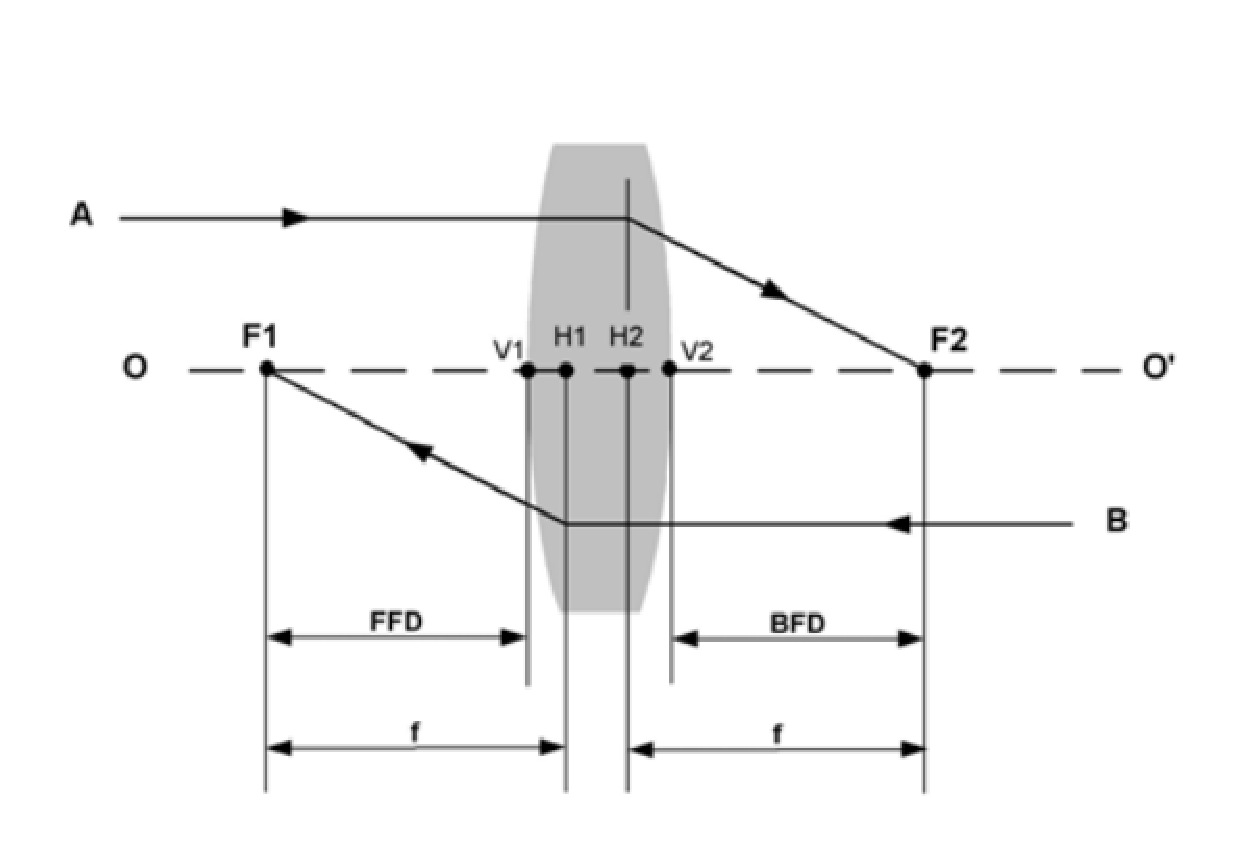
\includegraphics[width=0.6\textwidth]{bilder/lens_define}
\caption{The quantities define of singlet lenses \cite{lens_theory_LC_Ltd}}
\label{fig:lens_define}
\end{figure}
In order to understand more specifics about lenses Fig.\ref{fig:lens_define}  presents a singlet lens with geometric parameters. \"The optical axis (O-O')of the lens is a line passing through the centers of curvature of the two spherical lens surfaces. \"
Rays A and B, parallel with the optic axis (O-O'), are casted from different two sides through the lens and respectively cross the axis at their front and back focal points $F1$ and $F2$. The front and back principal points $H1$ and $H2$ are the intersections of the optical axis with the front and back principal surfaces. Points $V1$ and $V2$ are called the front and back vertices respectively\cite{lens_theory_LC_Ltd}.  Some important quantities are defined in Tab. \ref{tab:lens_quantities}. Here the distance $t_{c}$ is the center thickness of the lens $V1V2$.\\
\begin{table}
\centering
\caption{Important Quantities for Singlet Lenses Immersed in Air\cite{lens_theory_LC_Ltd}.}
\begin{tabular}{|c|c|c|}
\hline
\textbf{Symbol}&\textbf{Description}&\textbf{Formular}\\
\hline
$f$ & \parbox[c]{6cm}{
						\begin{center}
						effective focal length
						\end{center}
				}& $\frac{1}{f}=(n-1)\left[\frac{1}{R_{1}}-\frac{1}{R_{2}} \right]+\frac{t_{c}(n-1)^2}{nR_{1}R_{2}}$ \\
\hline
$BFD$ &\parbox[c]{6cm}{
						\begin{center}
						back focal distance 
						\end{center}
			}& $BFD=f\left[ 1-\frac{t_{c}(n-1)}{nR_{1}}\right]$ \\
\hline
$FFD$ &\parbox[c]{6cm}{
						\begin{center}
						 front focal distance
						 \end{center} 
			}& $FFD=f\left[ 1+\frac{t_{c}(n-1)}{nR_{1}}\right]$ \\
\hline
$H2V2$ & \parbox[c]{6cm}{
						\begin{center}
						back vertex to back principal point distance
						\end{center}						
			} & $H_{2}V_{2}=f-BFD=-f\frac{t_{c}(n-1)}{nR_{1}}$ \\
\hline
$V1H1$ & \parbox[c]{6cm}{
						\begin{center}			
				    front vertex to front principal point distance
				    \end{center}
				 } & $V_{1}H_{1}=f-FFD=-f\frac{t_{c}(n-1)}{nR_{2}}$ \\
\hline
\end{tabular}
\label{tab:lens_quantities}
\end{table}
The classical singlet lenses are plano convex, plano concave, equiconvex and equiconcave lenses, which are listed in following Tab.\ref{tab:lenses_focal_length} with their focal length relation.The performance of a lens is usually estimated by spot size and focal lengths. The definition of the spot size will be declared later in section \ref{sect:gaussian_beam}. The focal length is in common sense the distance from lens center to minimum spot. But this idea is not exact in any case.  Here we can testify this thought by Fig. \ref{fig:focal_length} and following equations (\ref{eq:snell_focal}-\ref{eq:focal_length}).\\
\begin{table}[!ht]
\centering
\caption{Focal length Formulas of Simple Singlet Lenses in Air and  
				 the Radii are considered positive in the formulas below\cite{lens_theory_LC_Ltd}.}
\begin{tabular}{|c|c|c|}
\hline
\textbf{Type}&\textbf{Description}&\textbf{Formula}\\
\hline
Plano Convex & \parbox[c]{2.1cm}{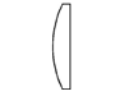
\includegraphics[width=2cm]{bilder/plano_convex}}& $f=\frac{R}{(n-1)}$ \\
\hline
Plano Concave &\parbox[c]{2.1cm}{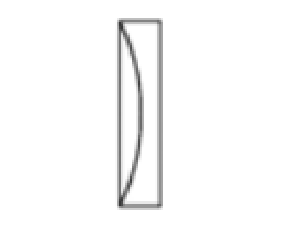
\includegraphics[width=2cm]{bilder/plano_concave}} & $f=-\frac{R}{(n-1)}$ \\
\hline
Equiconvex & \parbox[c]{2.1cm}{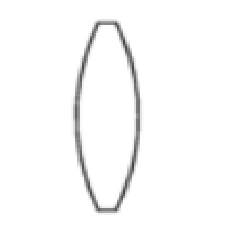
\includegraphics[width=2cm]{bilder/equi_convex}} & $f=\left[\frac{2(n-1)}{R} - \frac{t_{c}(n-1)^2}{nR^2}\right]^{-1}$ \\
\hline
Equiconcave & \parbox[c]{2.1cm}{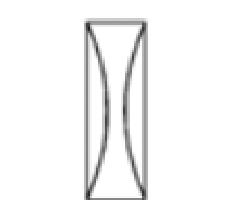
\includegraphics[width=2cm]{bilder/equi_concave}} & $f=\left[\frac{2(n-1)}{R} + \frac{t_{c}(n-1)^2}{nR^2}\right]^{-1}$ \\
\hline
\end{tabular}
\label{tab:lenses_focal_length}
\end{table}
\begin{figure}[!ht]
\centering
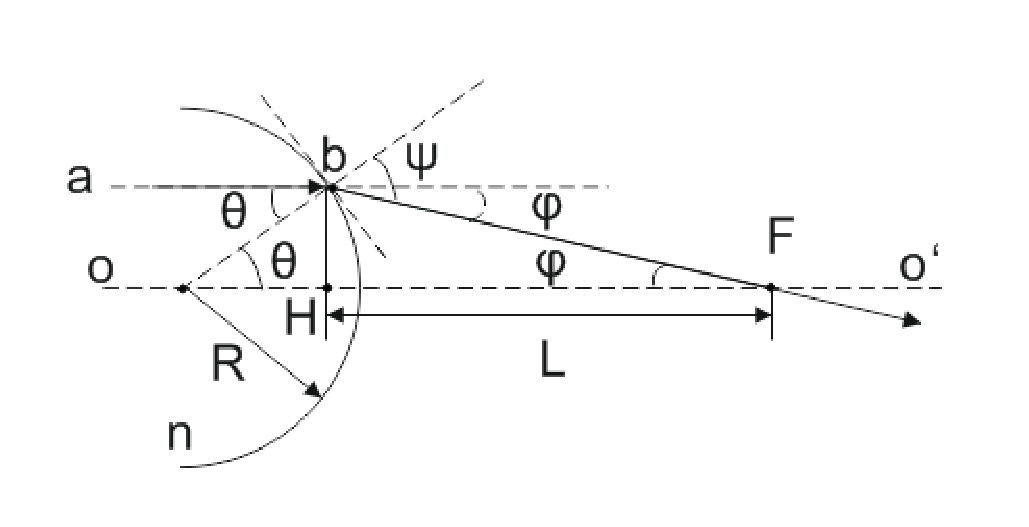
\includegraphics[width=0.6\textwidth]{bilder/focal_length}
\caption{Schema of refraction of parallel light by lens.}
\label{fig:focal_length}
\end{figure}

\begin{equation}
nsin\theta=sin\psi
\label{eq:snell_focal}
\end{equation}
\begin{equation}
\phi=\psi-\theta
\label{eq:psi_phi}
\end{equation}
\begin{align}
L&=Rsin(\theta) ctan(\phi) \nonumber\\
&=Rsin(\theta)\frac{cos(\psi-\theta)}{ sin(\psi-\theta)} \nonumber\\
&= Rsin(\theta)\frac{cos(\psi)cos(\theta)+sin(\psi)sin(\theta)}{sin(\psi)cos(\theta)-cos(\psi)sin(\theta)} \nonumber\\
&= Rsin(\theta)\frac{cos(\psi)cos(\theta)+nsin^{2}(\theta)}{nsin(\theta)cos(\theta)-cos(\psi)sin(\theta)} \nonumber\\
&=R\frac{cos(\psi)cos(\theta)+nsin^{2}(\theta)}{ncos(\theta)-cos(\psi)} \nonumber\\
&=R\frac{cos(\psi)cos(\theta)-ncos^{2}(\theta)+n}{ncos(\theta)-cos(\psi)} \nonumber\\
&=R \left[-cos(\theta)+\frac{n}{ncos(\theta)-\sqrt{1-n^{2}sin^{2}(\theta)}} \right]
\label{eq:focal_length}
\end{align}
In Fig. \ref{fig:focal_length} there is a lens with radius $R$ and index $n$. O-O' axis goes through the lens center.  The light source $a$ emits a ray parallel with the O-O' axis and at the point $b$ on the lens surface is refracted. At last the refracted ray cross the O-O' axis at point F. $\theta$ is the input angle, $\psi$ the output angle and $\phi$ the angle from output ray to O-O' axis. According the SNELL's LAW we get the relation between $\theta$ and $\psi$ in (\ref{eq:snell_focal}). $\phi$ and $\psi$ has the relation like (\ref{eq:psi_phi}). Then the distance $L$ from point H to F is given by (\ref{eq:focal_length}). When $\theta$ is close to 0 like (\ref{eq:focal_length_app}) $L$ is right equal the formula of Plano Convex in Tab. \ref{tab:lenses_focal_length}. So this formula of focal length is only valid for a small angle lens. 
\begin{equation}
L=R\left[ -1+\frac{n}{n-1}\right]=\frac{R}{n-1}
\label{eq:focal_length_app}
\end{equation}
Where is the focal point indeed located? \cite{lens_theory_LC_Ltd} has refered that the minimum spot lies between the maeginal plane and paraxial focal plane. All the distances which are in following discussed base on the assumption that the back vertex (V2) of the lens is regarded as origin. In Fig.\ref{fig:min_max_spot} there are "'geometrical traces of 25 rays in the focal region 100mm focal length plano convex lens(n=1.515)."'  "'The rays are launched parallel to the axis (O-O') and equally spaced in a region above and below the axis in a plane containing the axis(\textbf{meridional plane})"'. The marginal plane (\textbf{MP}) goes through the focal point of marginal rays. The paraxial focal plane (\textbf{PP}) goes through the focal point of paraxial rays. "'The distance from \textbf{PP} to \textbf{MP} is the \textbf{longitudinal aberration LAm}"'. The minimum spot (\textbf{MS}) is located at the plane, which is approximately 3/4 LAm back toward the lens from the \textbf{PP}.
\begin{figure}[httbp]
\centering
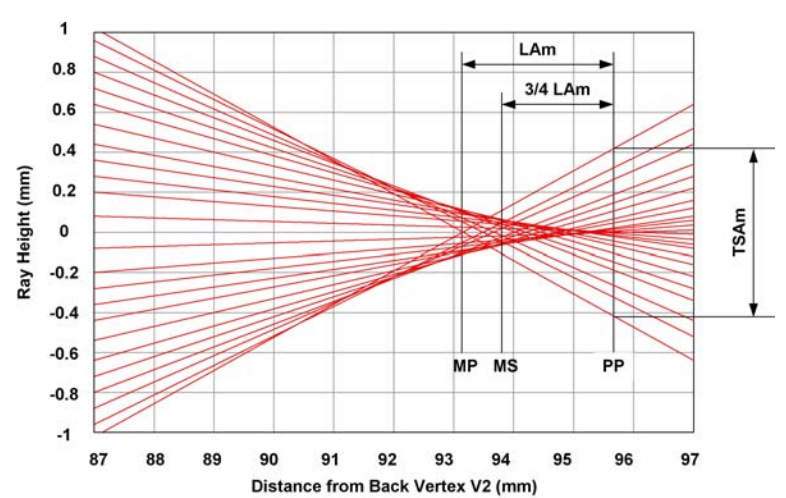
\includegraphics[width=0.9\textwidth]{bilder/min_max_spot}
\caption{Schema to estimating the minimum spot location \cite{lens_theory_LC_Ltd}.}
\label{fig:min_max_spot}
\end{figure}

\subsection{Fiber optics}
%Optical waveguides
For the transmission of optical signal optical waveguides are applied. The general waveguides are semiconductor waveguide and optical fibers. 
Fig. \ref{fig:semi_waveguides} shows two semiconductor waveguides commonly used in integrated optics. Rib waveguide is composed of a rib guide on a substrate ($n=n_{2}$). Buried waveguide is a high index guide ($n=n_{1}$) surrounded by low index cladding ($n=n_{2}$).\\
\begin{figure}
\centering
\subfigure[Rib waveguide]{
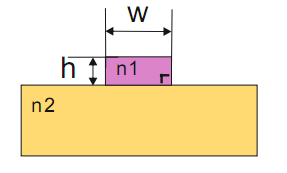
\includegraphics[width=0.4\textwidth]{bilder/approxmate_waveguide}
\label{fig:semi_rib_waveguide}
}
\hfill
\subfigure[Buried waveguide]{
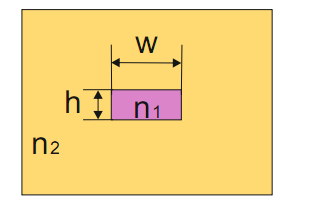
\includegraphics[width=0.4\textwidth]{bilder/buried_waveguide}
\label{fig:semi_buried_waveguide}
}
\caption{Schema of semiconductor waveguides}
\label{fig:semi_waveguides}
\end{figure}
Optical fibers are widely used for telecommunication and data networks. The Fig.\ref{fig:opticfiber} presents a simplest optical fiber and how lights propagate in the fiber . Optical fiber typically consists of a transparent core with index $n_{1}$ surrounded by a transparent cladding material with a lower index of refraction $n_{2}$. 
\begin{figure}[httbp]
\centering
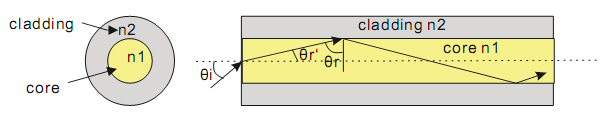
\includegraphics[width=0.8\textwidth]{bilder/opticfiber}
\caption{linght refraction in optic fibers}
\label{fig:opticfiber}
\end{figure}
\textbf{ Total Reflection}\\
\begin{figure}[!ht]
\centering
\subfigure[totalreflection]{
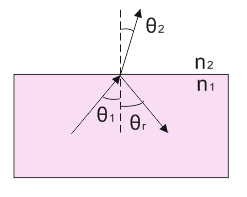
\includegraphics[width=0.3\textwidth]{bilder/totalreflection01}
\label{fig:totalreflection01}
}
\hfill
\subfigure[Buried waveguide]{
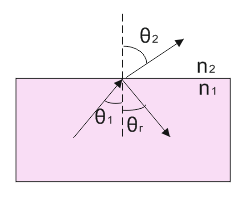
\includegraphics[width=0.3\textwidth]{bilder/totalreflection02}
\label{fig:totalreflection02}
}
\hfill
\subfigure[Buried waveguide]{
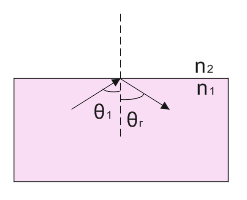
\includegraphics[width=0.3\textwidth]{bilder/totalreflection03}
\label{fig:totalreflection03}
}
\caption{Total reflection}
\label{fig:totalreflection}
\end{figure}

Whatever semiconductor waveguides or optical fibers, the principle of the light propagation in waveguides is total reflection. The principle of the total reflection is explained in \cite{optical_waveguides_fibers} with Snell's law. In Fig.\ref{fig:totalreflection01} the input light strikes the boundary between two different isotropic media with respective refractive index $n_{1}$ and $n_{2}$. Where $theta_{1}$ is incidence angle, $\theta_{2}$ refractive angle and $\theta_{r}$ reflective angle. Through SNELL's Law there are relations (\ref{eq:snell}-\ref{eq:reflection}).  For $n_{1}<n_{2}$ there is  always a relation $\theta_{1}>\theta_{2}$.  If the refractive indexes has the relation $n_{1}>n_{2}$, then the incidence angle $\theta_{1}$ is narrower than the refractive angle $\theta_{2}$ like Fig. \ref{fig:totalreflection02}. If the incidence angle is increased wider than a critical angle $\theta_{c}$ (\ref{eq:critical_angle}) there will be no light passing through the boundary and all of the lights are reflected like Fig. \ref{fig:totalreflection03}. This phenomenon is so called total reflection.
\begin{align}
n_{1}sin\theta_{1}&=n_{2}sin\theta_{2}
\label{eq:snell}\\
\theta_{1}=\theta{r}
\label{eq:reflection}
\end{align}
\begin{equation}
\theta_{c}=arcsin(\frac{n_{2}}{n_{1}})
\label{eq:critical_angle}
\end{equation}
%%dispersion
\textbf{ Numerical Aperture }\\
%Numerical Aperture
Another important character of optical waveguides is numerical aperture. Back to the Fig.\ref{fig:opticfiber} the incidence beam originate from the air into the fiber. There is a maximum coupling angle, so that the beam can be guided under the total reflecting conditions. Its sinus value (\ref{eq:NA}) is called \textbf{Numerical Aperture (NA)}, which indicate the acceptable range of ray beams.
\begin{align}
sin\theta_{i}&=\frac{n_{1}}{n_{0}}sin(90^{o}-\theta_{c})=n_{1}cos\theta_{c} \nonumber\\
&=n_{1}\sqrt{1-sin^{2}\theta_{c}}=n_{1}\sqrt{1-\left(\frac{n_{2}}{n_{1}}\right)^2}=\sqrt{n^2_{1}-n^2_{2}}
\label{eq:NA}
\end{align}
\textbf{Mode of the waveguide}\\
'An eigenmode $m$ of a waveguide structure is a propagation or evanescent wave which maintains its transverse shape during propagation '\cite{integrated_optics}. The eigenmode of a waveguide can be presented as (\ref{eq:e_eigenmode}-\ref{eq:h_eigenmode}). 
\begin{align}
E^{m}(r_{t},z)&=E^{m}_{0}(r_{t})e^{jk_{m}z}
\label{eq:e_eigenmode}\\
H^{m}(r_{t},z)&=H^{m}_{0}(r_{t})e^{jk_{m}z}
\label{eq:h_eigenmode}
\end{align}
Where $k_{m}$ is the propagation constant. When the request  $k_{0}n_{1}>k_{m}>k_{0}n_{2}$ is matched this mode is a guided mode for the waveguides \cite{script_FT_TET}. In this work the coupling bases on the fundamental mode.


\section{Gaussian Beam}
\labe{sect:gaussian_beam}
In the world there is no natural source of parallel beams. Each beam of light can be considered originating from a simple origin: point light source, which emits anisotropic light in all directions. Thus a normal light source cannot provide perfect focused beams for optical applications. TEM$_{00}$ mode of a laser source is a perfect plane wave with Gaussian transverse irradiance profile\cite{CVI_Melles_Griot_Technical_Guide}. Therefore the laser light is considered as a beam propagating in a well-defined direction with limited spreading in transversal dimensions.\\ 
In \cite{ script_FT_TET} the transversal e-field components of Gaussian beam is assumed as (\ref{eq:gaussian_01}).
\begin{equation}
E_{x}=\psi(x,y,z)e^{-jk_{0}nz}
\label{eq:gaussian_01}
\end{equation}
We insert (\ref{eq:gaussian_01}) into wave equation (\ref{eq:wave_equation})
\begin{equation}
\bigtriangleup E_{x}+k^{2}_{0}n^{2}E_{x}=0
\label{eq:wave_equation}
\end{equation}
 and obtain partial differential form (\ref{eq:gaussian_02}). Because the paraxial beams spread slowly in transversal direction due to the z-axis, the term $\frac{\partial ^{2}\psi}{\partial z^2}$ is very smaller than other terms. Thus equation (\ref{eq:gaussian_02}) become an approximation (\ref{eq:gaussian_03}).
\begin{equation}
\frac{\partial ^{2}\psi}{\partial x^2}+\frac{\partial ^{2}\psi}{\partial y^2}+\frac{ \partial ^{2}\psi}{\partial z^2}-2jk_{0}n\frac{\partial\psi}{\partial z}=0
\label{eq:gaussian_02}
\end{equation}
\begin{equation}
\frac{ \partial ^{2}\psi}{\partial x^2}+\frac{\partial ^{2}\psi}{\partial y^2}-2jk_{0}n\frac{\partial\psi}{\partial z}=0
\label{eq:gaussian_03}
\end{equation}
The equation(\ref{eq:gaussian_03}) can also be transformed into cylinder coordinate and become (\ref{eq:gaussian_04})
\begin{equation}
\frac{1}{r}\frac{\partial}{\partial r}\left(r\frac{\partial z}{\partial r}\right)+\frac{1}{r^2}\frac{ \partial ^{2}\psi}{\partial \phi^2}-2jk_{0}n\frac{\partial\psi}{\partial z}=0
\label{eq:gaussian_04}
\end{equation}
(\ref{eq:gaussian_05}) is one general solution of (\ref{eq:gaussian_04})
\begin{equation}
\psi(r,z)=\psi_{0}\exp\left(-j\left[P(z)+2 \frac{ k_{0}n}{2q(z)}r^2\right]\right)
\label{eq:gaussian_05}
\end{equation}
Where $P(z)$ and $q(z)$ meet the equation (\ref{eq:gaussian_04}) for any $r$. The term $q(z)$ has also the relation (\ref{eq:gaussian_06}) with some physical variables $w(z)$ and $R(z)$
\begin{equation}
\frac{1}{q(z)}=\frac{1}{R(z)}-\frac{j\lambda}{\pi nw^{2}(z)}
\label{eq:gaussian_06}
\end{equation}
Where $w(z)$ is the $1/e^2$ irradiance radius due to propagating distance z and $R(z)$ is the wavefront radius of curvature due to propagating distance z
\begin{equation}
w(z)=w_{0}\sqrt{1+\left(\frac{\lambda z}{n\pi w^{2}_{0}}\right)^{2}}
\label{eq:gaussian_07}
\end{equation}
\begin{equation}
R(z)=z\left[1+\left(\frac{\lambda z}{n\pi w^{2}_{0}}\right)^{2}\right]
\label{eq:gaussian_08}
\end{equation}

If (\ref{eq:gaussian_06}) is inserted in (\ref{eq:gaussian_05}) then we can obtain a Gauss form result 
\begin{equation}
\psi(r,z)=w_{0}\exp\left(-\frac{r^2}{w^2_{0}}\right) \text{.}
\label{eq:gaussian_09}
\end{equation}
That means the field of a Gaussian beam is in transversal dimensions a Gaussian distribution like Fig. \ref{fig:gaussian_verteilung}.\\

\begin{figure}[!ht]
\centering
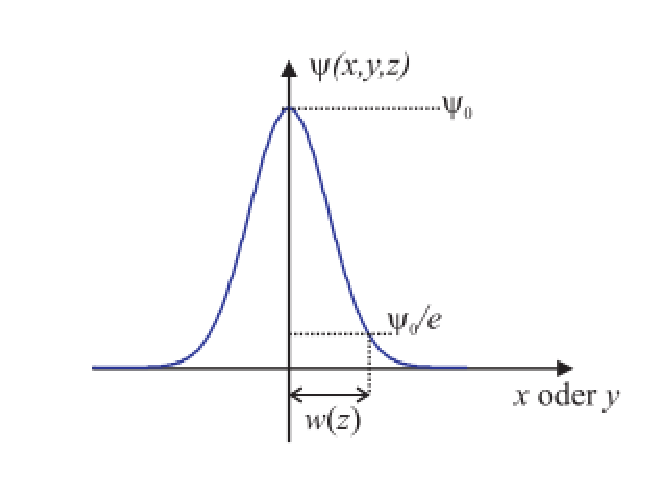
\includegraphics[width=0.6\textwidth]{bilder/gussian_verteilung}
\caption{Transversal profile of the Gaussian beam is the curve of Gaussian functions. At the beam center the field has the maximum value. At the distance of $w(z)$ form the center the field decline to $1/e$ of the peak value.}
\label{fig:gaussian_verteilung}
\end{figure}
According to definitions of $w(z)$ and $R(z)$ in (\ref{eq:gaussian_07}-\ref{eq:gaussian_08}) the longitudinal profile of Gaussian beams can be drawn as Fig. \ref{fig:gussian_profile}.
\begin{figure}[!ht]
\centering
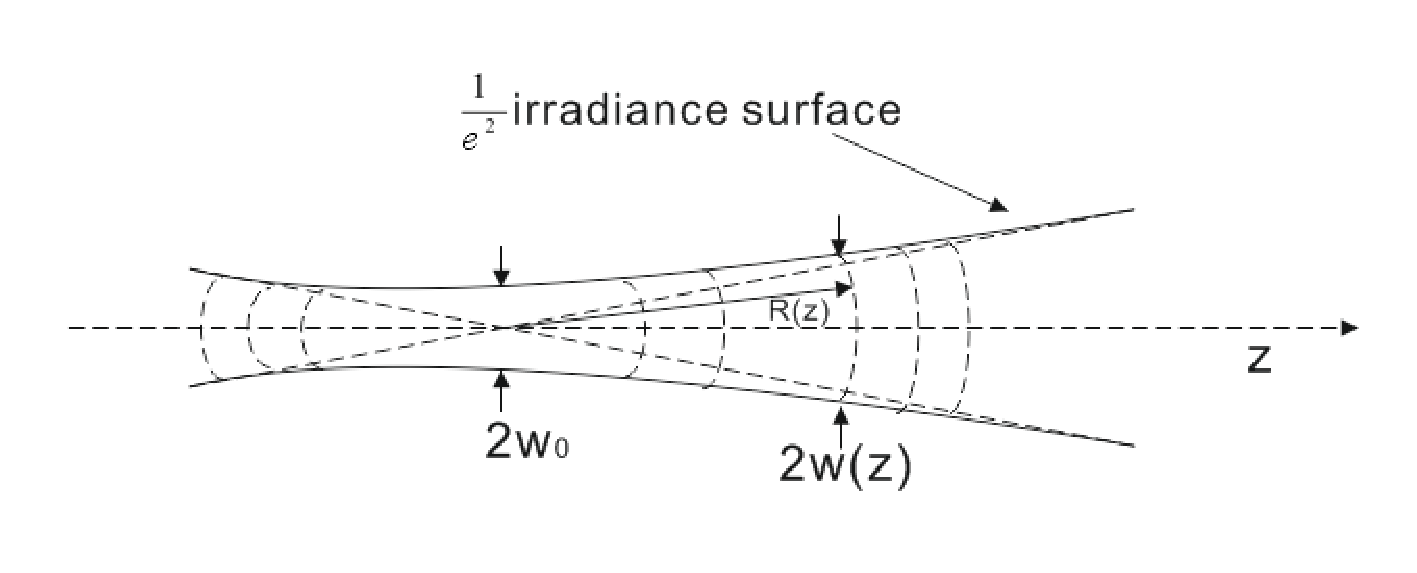
\includegraphics[width=0.9\textwidth]{bilder/gussian_profile}
\caption{The lateral profile of Gaussian beams presents the domain of beam power from peak value to $1/e^2$ peak value. $w(z)$ represents the radius of this profile. $R(z)$ is the radius of wavefronts.}
\label{fig:gussian_profile}
\end{figure}
From the beam axis to the distance of beam radius $w(z)$ the intensity drops to $1/e^{2}$ (about $ 13.5\%$) of the maximum value. That means, a hard aperture with radius $w$ can transmit about $86.5\%$ of the optical power.

%Spot Size
\subsubsection*{Spot Size}
Another important characteristic of Gaussian beams is Spot Size. In a cross-section of a Gaussian beam the beam intensity is approximately distributed as Gaussian function. The spot size is the diameter of the domain at whose edge the value of the electrical field intensity decays to $1/e$ of the peak value, otherwise the energy density decays to $1/e^2$ of the peak value.


\section{Finite Integration Method}
The Finite Integration Theory(\textbf{FIT}), which was introduced at 1976 by Thomas Weiland\cite{FIT_discrete_method} to solving the electromagnetical problems, is a numerical simulation method to discretize the integral form of fundamental Maxwell's functions.

The first thought of the \textbf{FIT} is to discretize the calculating volume. There is lot of methods to accomplish this mission. One common way is as Fig.\ref{fig:discretization_material} to discetize a brick-shape object into a \textbf{Cartesian Grid}(primary cell \textbf{G}). Of cause it is possible to construct grid volume in cylinder coordinate or any other types of  coordinates\cite{FIT_triangular_discretization,FDTD_nonorthogonal_grids} for simplifying the calculation depending on the real dimensions of the object. In general \cite{script_FeldSim} indicate the computational grid as (\ref{eq:grid}).
\begin{equation}
G={(u(i),v(j),w(k))\in R^3|u(1)\leq u(i)\leq u(I),
													 v(1)\leq v(j)\leq v(J),
													 w(1)\leq w(k)\leq w(K)
}
\label{eq:grid}
\end{equation}
$u(i),v(j),w(k)$ can be three components of any 3D coordinate systems. In following discussion all computations base on \textbf{Cartesian Coordinate system}.
%fig: discretization of the material
\begin{figure}[!ht]
\centering
%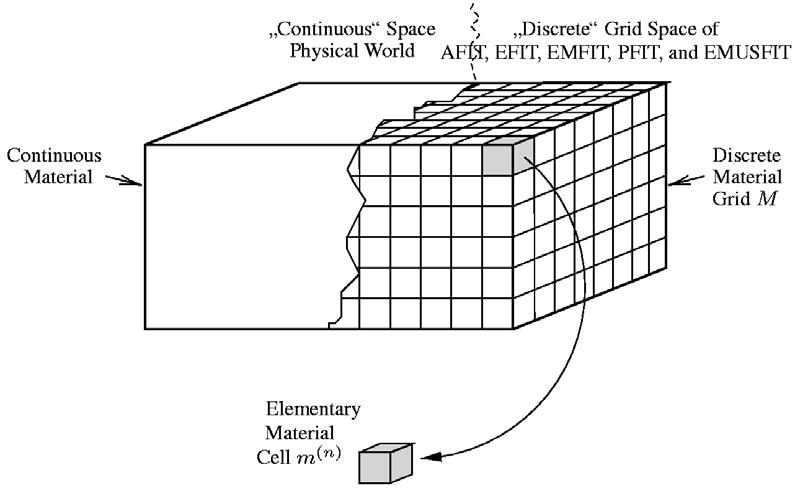
\includegraphics[width=0.8\textwidth]{bilder/discretization_material}
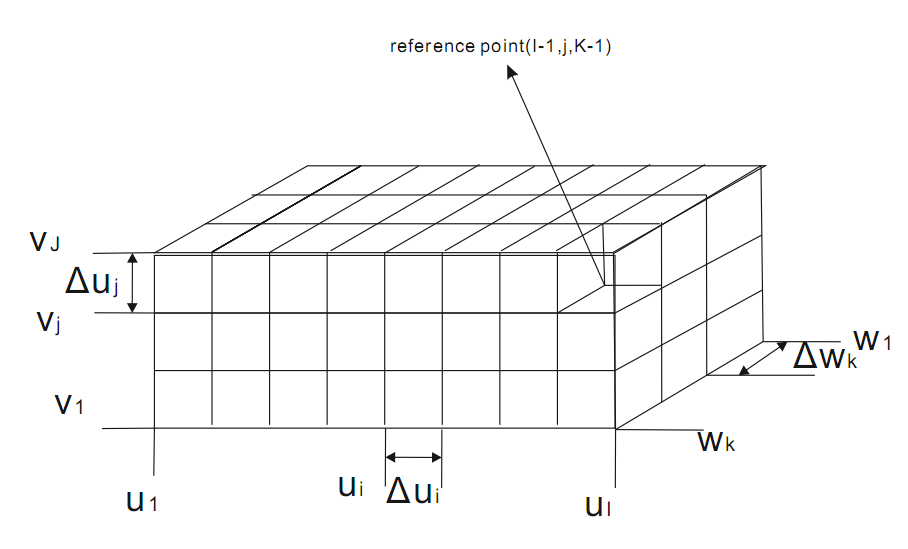
\includegraphics[width=0.8\textwidth]{bilder/grid_volum}
%\caption{A discretization of the material in elementary material cells m, defining the material grid M.}
\caption{A Cartesian descretized Grid Volum.}
\label{fig:discretization_material}
\end{figure}


In \cite{script_FeldSim} the primary elements are chosen for calculation:
\begin{itemize}
\item Points $P(i,j,k)$
\item Elemental Edge:
%$\delta u(i)=\overline{u(i)u(i+1)} with 1\leq{i}\leq{I-1},$
    \begin{align}
		\Delta u(i)&=\overline{u(i)u(i+1)}  \quad with  \quad 1\leq i \leq I-1, \nonumber\\
		\Delta v(j)&=\overline{v(j)v(j+1)}  \quad with  \quad 1\leq j \leq J-1, \nonumber\\
		\Delta w(k)&=\overline{w(k)w(k+1)}  \quad with  \quad 1\leq k \leq K-1
		\label{eq:discrete_edge}
		\end{align}
\item Elemental Planes
		\begin{align}
		A_{u}(j,k)&=\Delta v(j)\Delta w(k) \quad with  \quad 1\leq i \leq I-1,1\leq j \leq J-1\nonumber\\
		&A_{v}(i,k),A_{w}(i,j)  \quad analogous
		\label{eq:discrete_plane}
		\end{align}
\item Elemental Cells
		\begin{equation}
		V(i,j,k)=\Delta u(i)\Delta v(j)\Delta w(k)  \quad with  \quad 1\leq i\leq I-1,1\leq j\leq J-1,1\leq k\leq K-1
		\label{eq:discrete_cell}
		\end{equation}
\end{itemize}
For the convenience a new index system is introduced:

\begin{equation}
n=1+(i-1)\cdot M_{u}+(j-1)\cdot M_{v}+(k-1)\cdot M{w}
\label{eq:discrete_index}
\end{equation}
Here $M_{u}=1,M_{v}=I,M_{w}=I\cdot J$. With new index
Reindex points $P(i,j,k)$ with $n$. Same work is done for element edges, planes and volumes, new elements sequence are created:
\begin{itemize}
\item Points $P(n) \quad with \quad 1\leq n \leq N_{p}$
\item Elemental Edge:
%$\delta u(i)=\overline{u(i)u(i+1)} with 1\leq{i}\leq{I-1},$
    \begin{align}
		\Delta u(n)&=\overline{u(n)u(n+1)}  \quad with \quad 1\leq n \leq N_{p}, \nonumber\\
		\Delta v(n)&=\overline{v(n)v(n+1)}  \quad with \quad 1\leq n \leq N_{p}, \nonumber\\
		\Delta w(n)&=\overline{w(n)w(n+1)}  \quad with \quad 1\leq n \leq N_{p}
		\label{eq:discrete_edge_n}
		\end{align}
\item Elemental Planes
		\begin{align}
		A_{u}(n)&=\Delta v(n)\Delta w(n) \quad with \quad 1\leq n\leq N_{p}\nonumber\\
		&A_{v}(n),A_{w}(n)  \quad analogous
		\label{eq:discrete_plane_n}
		\end{align}
\item Elemental Cells
		\begin{equation}
		V(n)=\Delta u(n)\Delta v(n)\Delta w(n)  \quad with \quad 1\leq n\leq N_{p}
		\label{eq:discrete_cell_n}
		\end{equation}
\end{itemize}
Here, $N_{p}$ is the total number of the grid points:
\begin{equation}
N_{p}=I\cdot J\cdot K
\label{eq:np}
\end{equation}

The next step is to discretize Maxwell's equations in their integral form(\ref{eq:maxwell_1}-\ref{eq:maxwell_4}) and additional equations (\ref{eq:maxwell_5}-\ref{eq:maxwell_7}).

\begin{align}
\oint_{\partial A}\vec{E}\cdot\mathrm{d}\vec{s}&=
-\frac{\mathrm{d}}{\mathrm{d}t}\int_{A}\vec{B}\cdot\mathrm{d}\vec{A}
\label{eq:maxwell_1}\\
\oint_{\partial A}\vec{H}\cdot\mathrm{d}\vec{s}&=
\int_{A}(\frac{\partial\vec{D}}{\partial t}+\vec{J})\cdot\mathrm{d}\vec{A}
\label{eq:maxwell_2}\\
\oint_{\partial V}\vec{D}\cdot\mathrm{d}\vec{A}&=
\int_{V}\rho\mathrm{d}V
\label{eq:maxwell_3}\\
\oint_{\partial V}\vec{B}\cdot\mathrm{d}\vec{A}&=0
\label{eq:maxwell_4}
\end{align}
Additional equations:
\begin{align}
\vec{D}&=\epsilon_{0}\epsilon_{r}\vec{E}
\label{eq:maxwell_5}\\
\vec{B}&=\mu_{0}\mu_{r}\vec{H}
\label{eq:maxwell_6}\\
\vec{J}&=\kappa\vec{E}+\vec{J_{s}}
\label{eq:maxwell_7}
\end{align}

%%law inductive

Following is a demonstration of the discretized form from the inductive law (\ref{eq:maxwell_1}). Considering the path integral in a single element edge like Fig.  \ref{fig:FIT_max_integral1},the left side of (\ref{eq:maxwell_1}) can be presented as  (\ref{eq:inductive_left}). 

\begin{figure}[!ht]
\centering
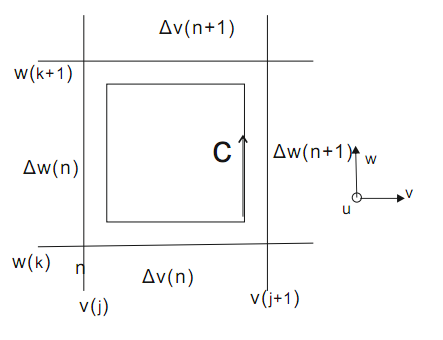
\includegraphics[width=0.45\textwidth]{bilder/FIT_max_integral1}
\caption{ Path integral along edges of one single elemental plane $A_{u}(n)$\cite{ script_FeldSim}.}
\label{fig:FIT_max_integral1}
\end{figure}

\begin{figure}[!ht]
\centering
\subfigure[Discrete electric field strength components distribute at edges of grids.]{
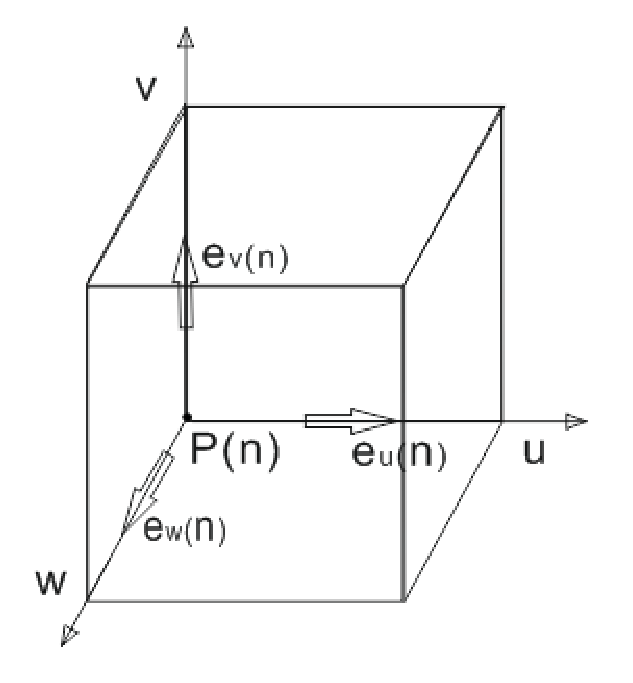
\includegraphics[width=0.4\textwidth]{bilder/FIT_max_integral2}
\label{fig:FIT_max_integral2}
}
\hfill
\subfigure[Discrete magnetic flux density components distribute at planes of grids.]{
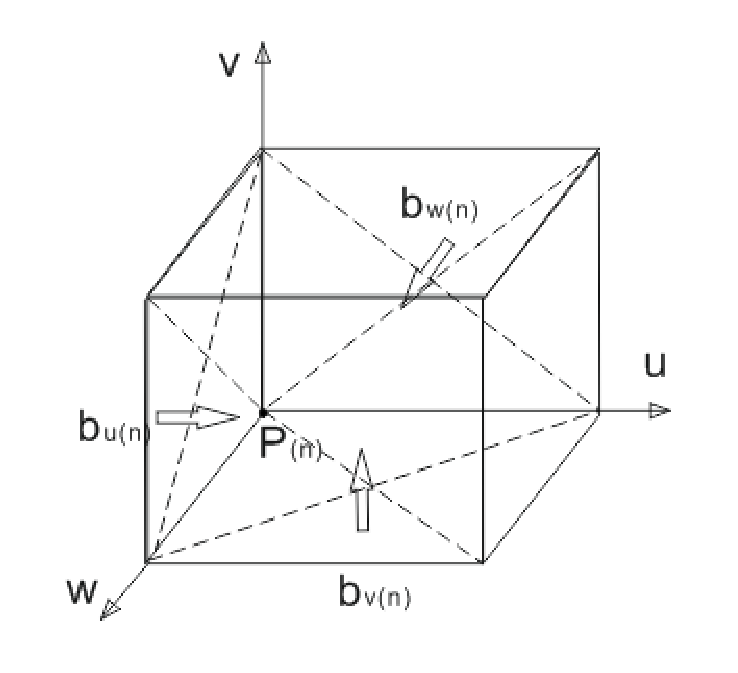
\includegraphics[width=0.5\textwidth]{bilder/FIT_max_integral3}
\label{fig:FIT_max_integral3}
}
\caption{Allocations of components at grids\cite{ script_FeldSim}.}
\end{figure}

\begin{equation}
\int_{C}\vec{E}\cdot d\vec{s}
=\underbrace{\int_{\Delta v(n)}\vec{E}\cdot d\vec{s}}_{\widehat{e}_{v}(n)}
+\underbrace{\int_{\Delta w(n+M_{v})}\vec{E}\cdot d\vec{s}}_{\widehat{e}_{w}(n+M_{v})}
-\underbrace{\int_{\Delta v(n+M_{w})}\vec{E}\cdot d\vec{s}}_{\widehat{e}_{v}(n+M_{w})}
-\underbrace{\int_{\Delta w(n)}\vec{E}\cdot d\vec{s}}_{\widehat{e}_{w}(n)}
\label{eq:inductive_left}
\end{equation}

Where $\widehat{e}(n)$ is so called  electric grid voltage and has the following relation with electric field strength $e(n)$
\begin{equation}
 e_{v}(n)=\frac{\widehat{e}_{v}(n)}{\Delta v(n)}
\label{eq:e_field}
\end{equation}
Meanwhile the right hand side of (\ref{eq:maxwell_1}) approximates to (\ref{eq:inductive_right})
\begin{equation}
-\iint_{A_{u}(n)}\frac{\partial\vec{B}}{\partial t}\cdot\mathrm{d}\vec{A} 
=-\iint_{A_{u}(n)}\frac{\partial B^{*}_{u}}{\partial t}\cdot\mathrm{d}A
\approx -\frac{\partial}{\partial t}b_{u}(n)A_{u}(n)
\label{eq:inductive_right}
\end{equation}
Where $A_{u}(n)=\Delta v(n)\Delta w(n)$ and $b_{u}(n)$ (Fig.\ref{fig:FIT_max_integral2}) is magnetic flux density, given by
\begin{equation}
 b_{u}(n)=\frac{\widehat{\widehat{b}}_{u}(n)}{\Delta A_{u}(n)} \text{,}
\label{eq:b_flux_density}
\end{equation}
 and magnetic grid flux $\widehat{\widehat{b}}_{u}(n)$, given by
\begin{equation}
\widehat{\widehat{b}}_{u}(n)=\iint_{A_{u}(n)}\vec{B}\cdot\mathrm{d}\vec{A} \text{.}
\label{eq:mag_fluxe}
\end{equation}
From equations (\ref{eq:inductive_left}-\ref{eq:mag_fluxe}) we obtain the difference form (\ref{eq:inductive_integral}) of the inductive equation at one single elemental plane:
\begin{equation}
\widehat{e}_{v}(n)+\widehat{e}_{w}(n+M_{v})-\widehat{e}_{v}(n+M_{w})-\widehat{e}_{w}(n)=-\frac{\partial}{\partial t}\widehat{\widehat{b}}_{u}(n)
\label{eq:inductive_integral}
\end{equation}
i.e.,
\begin{align}
\Delta v(n)e_{v}(n)&+\Delta w(n+M_{v})e_{w}(n+M_{v})\nonumber\\
-\Delta v(n+M_{w})e_{v}(n+M_{w})&-\Delta w(n)e_{w}(n)=-A_{u}(n)\frac{\partial}{\partial{t}}b_{u}(n) 
\label{eq:inductive_sample}
\end{align}
By merging electric field-strength $e(n)$ and magnetic flux density $b(n)$ of all grids into vectors we obtain:
\begin{equation*}
e_{u}:=
\begin{pmatrix}
e_{u}(1)&\\
\vdots&\\
e_{u}(N_{p})&
\end{pmatrix},
e_{v}:=
\begin{pmatrix}
e_{v}(1)&\\
\vdots&\\
e_{v}(N_{p})&
\end{pmatrix},
e_{w}:=
\begin{pmatrix}
e_{w}(1)&\\
\vdots&\\
e_{w}(N_{p})&
\end{pmatrix},
e:=
\begin{pmatrix}
e_{u}&\\
e_{v}&\\
e_{w}&
\end{pmatrix},
\label{eq:vector_e_field}
\end{equation*}
\begin{equation*}
b_{u}:=
\begin{pmatrix}
b_{u}(1)&\\
\vdots&\\
b_{u}(N_{p})&
\end{pmatrix},
b_{v}:=
\begin{pmatrix}
b_{v}(1)&\\
\vdots&\\
b_{v}(N_{p})&
\end{pmatrix},
b_{w}:=
\begin{pmatrix}
b_{w}(1)&\\
\vdots&\\
b_{w}(N_{p})&
\end{pmatrix},
b:=
\begin{pmatrix}
b_{u}&\\
b_{v}&\\
b_{w}&
\end{pmatrix}.
\label{eq:vector_m_flux_density}
\end{equation*}
Expanding the relation (\ref{eq:inductive_sample}) to all grid cells \cite{FIT_discrete_method,FIT_discrete_electrommagnetism} we arrive at the discrete form of inductive equation:
\begin{equation}
CD_{s}e=-D_{A}\frac{\partial}{\partial{t}}b
\label{eq:inductive_sample_all}
\end{equation}
Where $D_{s}$ is elemental edge matrix, given by
\begin{align*}
D_{s}=
%	\begin{pmatrix}
%	\Delta u(1)&&&&&&&&\\
%	&\ddots &&&&&&&\\
%	&&\Delta u(N_{p})&&&&&&\\
%	&&&\Delta v(1)&&&&&\\
%	&&&&\ddots &&&&\\
%	&&&&&\Delta v(N_{p})&&&\\
%	&&&&&&\Delta w(1)&&\\
%	&&&&&&&\ddots &\\
%	&&&&&&&&\Delta w(N_{p})
%	\end{pmatrix}
Diag\{&\Delta u(1),\cdots,\Delta u(N_{p}),\nonumber\\
			&\Delta v(1),\cdots,\Delta v(N_{p}),\nonumber\\
			&\Delta w(1),\cdots,\Delta w(N_{p})
\} \text{.}
	%\label{eq:Ds_matrix}
\end{align*}
$D_{A}$ is elemental plane matrix, given by
\begin{align*}
D_{A}=
%	\begin{pmatrix}
%	\Delta A_{u}(1)&&&&&&&&\\
%	&\ddots &&&&&&&\\
%	&&\Delta A_{u}(N_{p})&&&&&&\\
%	&&&\Delta A_{v}(1)&&&&&\\
%	&&&&\ddots &&&&\\
%	&&&&&\Delta A_{v}(N_{p})&&&\\
%	&&&&&&\Delta A_{w}(1)&&\\
%	&&&&&&&\ddots &\\
%	&&&&&&&&\Delta A_{w}(N_{p})
%	\end{pmatrix}
Diag\{&\Delta A_{u}(1),\cdots,\Delta A_{u}(N_{p}),\nonumber\\
			&\Delta A_{v}(1),\cdots,\Delta A_{v}(N_{p}),\nonumber\\
			&\Delta A_{w}(1),\cdots,\Delta A_{w}(N_{p})
\} \text{.}
	%\label{eq:Da_matrix}
\end{align*}
$C$ is \textbf{curl} operator, given by
\begin{align*}
C&=\left(
	\begin{array}{ccc|ccc|ccc}
	&&&\ddots &-1& &\ddots &+1&\\	
	&0&&&+1&\ddots&&-1&\ddots\\
	&&&&&\ddots&&&\ddots\\	
	\hline
	\ddots &+1&&&&&\ddots &-1&\\
	&-1 &\ddots&&0&\quad&&+1&\ddots\\
	&&\ddots&&&&&&\ddots\\
	\hline
	\ddots &-1&&\ddots &+1&&&&\\
	&+1 &\ddots&&-1&\ddots&&0&\\
	&&\ddots&&&\ddots&&&
	\end{array}\right)\\
	&=
	\begin{pmatrix}
	0&-P_{w}&P_{v}\\
	P_{w}&0&-P_{u}\\
	-P_{v}&P_{u}&0
	\end{pmatrix} \text{.}
%\label{eq:C_matrix}
\end{align*}
\begin{figure}[!ht]
\centering
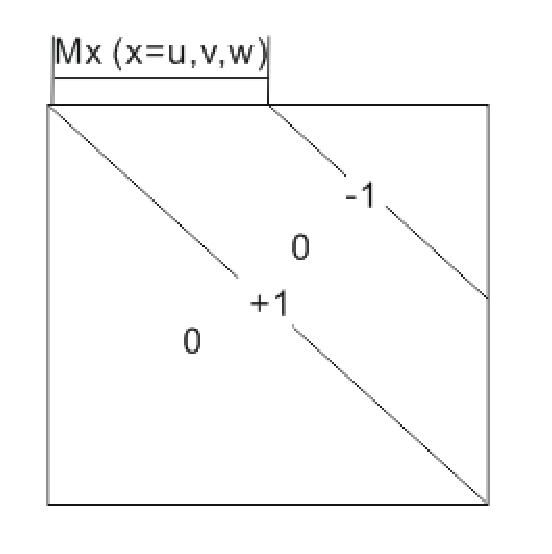
\includegraphics[width=0.4\textwidth]{bilder/P_matrix}
\caption{Structure of matrix $P_{x},(x=u,v,w)$.}
\label{fig:Matrix Px}
\end{figure}
Submatrices $P_{u},P_{v},P_{w}$ are composed of $1,-1,0$ like Fig. \ref{fig:Matrix Px}.\\
 
Alternative form of the equation (\ref{eq:inductive_sample_all}) is given in (\ref{eq:inductive_integral_all})
\begin{equation}
C\widehat{e}=-\frac{\partial}{\partial{t}}\widehat{\widehat{b}}
\label{eq:inductive_integral_all}
\end{equation}
%\widehat{e}
Where electric voltage $\widehat{e}$ and magnetic flux $\widehat{ \widehat{b}}$ are defined as following:
\begin{equation}
\widehat{e}_{u}:=
\begin{pmatrix}
\widehat{e}_{u}(1)&\\
\vdots&\\
\widehat{e}_{u}(N_{p})&
\end{pmatrix},
\widehat{e}_{v}:=
\begin{pmatrix}
\widehat{e}_{v}(1)&\\
\vdots&\\
\widehat{e}_{v}(N_{p})&
\end{pmatrix},
\widehat{e}_{w}:=
\begin{pmatrix}
\widehat{e}_{w}(1)&\\
\vdots&\\
\widehat{e}_{w}(N_{p})&
\end{pmatrix},
\widehat{e}:=
\begin{pmatrix}
\widehat{e}_{u}&\\
\widehat{e}_{v}&\\
\widehat{e}_{w}&
\end{pmatrix},
\label{eq:vector_e_voltage}
\end{equation}
%\widehat{\widehat{b}}
\begin{equation}
\widehat{\widehat{b}}_{u}:=
\begin{pmatrix}
\widehat{\widehat{b}}_{u}(1)&\\
\vdots&\\
\widehat{\widehat{b}}_{u}(N_{p})&
\end{pmatrix},
\widehat{\widehat{b}}_{v}:=
\begin{pmatrix}
\widehat{\widehat{b}}_{v}(1)&\\
\vdots&\\
\widehat{\widehat{b}}_{v}(N_{p})&
\end{pmatrix},
\widehat{\widehat{b}}_{w}:=
\begin{pmatrix}
\widehat{\widehat{b}}_{w}(1)&\\
\vdots&\\
\widehat{\widehat{b}}_{w}(N_{p})&
\end{pmatrix},
\widehat{\widehat{b}}:=
\begin{pmatrix}
\widehat{\widehat{b}}_{u}&\\
\widehat{\widehat{b}}_{v}&\\
\widehat{\widehat{b}}_{w}&
\end{pmatrix}.
\label{eq:vector_m_flux}
\end{equation}
%divergence equation
\begin{figure}[!ht]
\centering
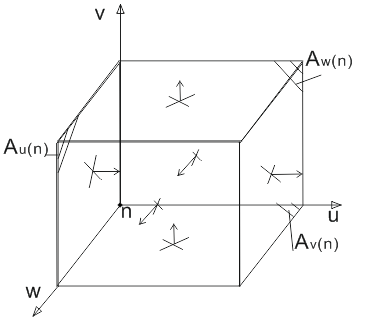
\includegraphics[width=0.5\textwidth]{bilder/divergence_in_grid}
\caption{This figure discribe the allocation of six magnetic facet fluxes in $G$.}
\label{fig:divergence_G}
\end{figure}
Analogy the divergence equation (\ref{eq:maxwell_4}) can also be discretized in grid $G$ and through Fig.\ref{fig:divergence_G} we obtain difference form: 
\begin{equation}
SD_{A}b=0
\label{eq:divergence_sample}
\end{equation}
or
\begin{equation}
S\widehat{\widehat{b}}=0
\label{eq:divergence_integral}
\end{equation}
$S\in \mathbb{R}^{N_{p}\times 3N_{p}}$ represent the discrete divergence matrix, which depends on the grid topology just as the discrete $curl-Matrix$ $C$.
%S
\begin{equation}
S=(P_{u}|P_{v}|P_{w})
\label{eq:S_matrix}
\end{equation}
%Amp\'ere's law
Now considering the discretization of Amp\'ere's law (\ref{eq:maxwell_2}) its magnetic field strengths pass through the elemental plane along the same path with the magnetic flux density (Fig. \ref{fig:divergence_G}). Therefore, a new grid (\textbf{Dual Grid}) like Fig. \ref{fig:dual_grid} is required for this path integral. The second cell $\tilde{G}$ is dual to the primary grid $G$. As primary elements in primary Grid the dual elements are also properly defined in \cite{script_FeldSim}.
\begin{figure}[!ht]
\centering
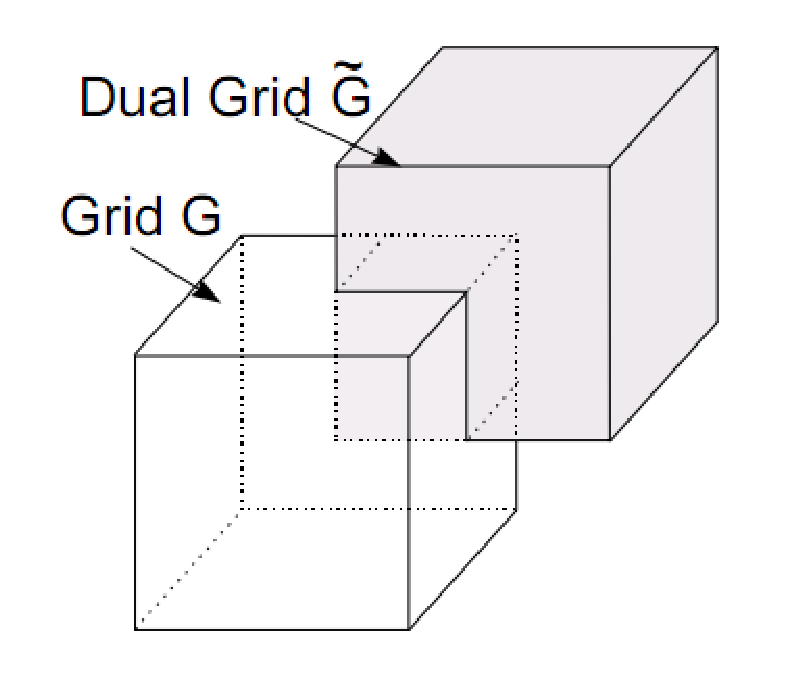
\includegraphics[width=0.5\textwidth]{bilder/dual_grid}
\caption{The allocation of the Primary Grid $G$ and Dual Grid $\tilde{G}$\cite{FIT_discrete_electrommagnetism}.}
\label{fig:dual_grid}
\end{figure}
Like the discretization of Inductive Law Figure. \ref{fig:FIT_max_integral4} and Figure.  \ref{fig:FIT_max_integral5} describe the path integral and surface integral of the equation(\ref{eq:maxwell_2}) in a \textbf{Dual Grid} and lead to the difference equations (\ref{eq:ampere_left_sample}-\ref{eq:ampere_right}).
\begin{figure}
%\centering
	\subfigure[Path Integral of the magnetic flux in dual grid.]{	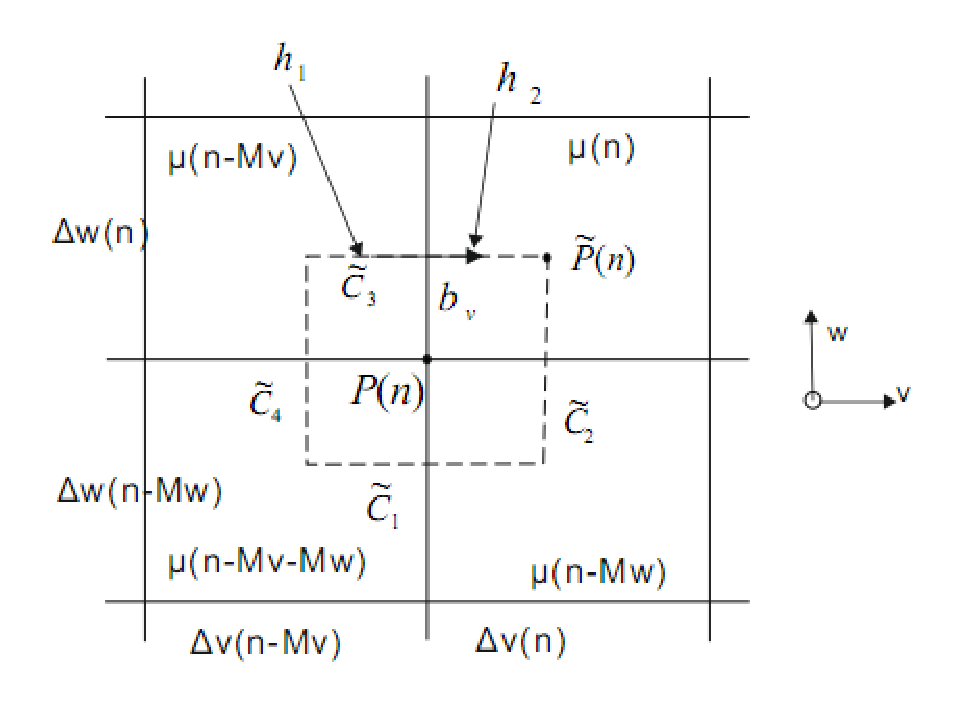
\includegraphics[width=0.5\textwidth]{bilder/FIT_max_integral4}
	\label{fig:FIT_max_integral4}
	}
\hfill
	\subfigure[Surface Integral of the electric flux in dual grid.]{	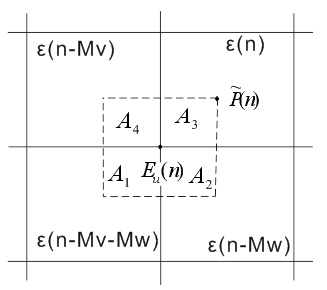
\includegraphics[width=0.4\textwidth]{bilder/FIT_max_integral5}
	\label{fig:FIT_max_integral5}
	}
\caption{Discretization of Amp\'ere's law.}
\end{figure}
\begin{equation}
\int_{\tilde{C}}\vec{H}\cdot d\vec{s}=\int_{\tilde{C}}\mu^{-1}\vec{B}\cdot d\vec{s}\approx
\widehat{h}_{v}(n)
+\widehat{h}_{w}(n+M_{v})
-\widehat{h}_{v}(n+M_{w})
-\widehat{h}_{w}(n)
\label{eq:ampere_left_sample}
\end{equation}
\begin{align}
\int\int_{\tilde{A}_{u}}\vec{D}\cdot\mathrm{d}\vec{A}\approx &+e_{u}A_{1}\epsilon_{u}(n-M_{v}-M_{w}) \nonumber\\
&+e_{u}A_{2}\epsilon_{u}(n-M_{w}) \nonumber\\
&+e_{u}A_{3}\epsilon_{u}(n) \nonumber\\
&+e_{u}A_{4}\epsilon_{u}(n-M_{v}) \nonumber\\
&=\bar{\epsilon}_{u}(n)e_{u}\tilde{A}_{u}
\label{eq:ampere_right}
\end{align}
with 
\begin{equation}
\widehat{h}_{v}(n)=h_{1}\cdot\frac{\Delta v(n-M_{v})}{2}+ h_{2}\cdot\frac{\Delta v(n)}{2}
\label{eq:megnetic_field1}
\end{equation}
\begin{equation}
h_{1}=\frac{b_{v}(n)}{\mu (n-M_{v})}
\label{eq:megnetic_field2}
\end{equation}
\begin{equation}
h_{2}=\frac{b_{v}(n)}{\mu (n)}
\label{eq:megnetic_field3}
\end{equation}
\begin{equation}
A_{1}=\frac{A_{u}(n-M_{v}-M_{w})}{4}
\end{equation}
\begin{equation}
A_{2}=\frac{A_{u}(n-M_{w})}{4}
\end{equation}
\begin{equation}
A_{3}=\frac{A_{u}(n)}{4}
\end{equation}
\begin{equation}
A_{4}=\frac{A_{u}(n-M_{v})}{4}
\end{equation}
\begin{align}
\bar{\epsilon}_{x}(n)&:=\frac{\int\int\epsilon\mathrm{d}A}{\int\int\mathrm{d}A}\nonumber\\
&=\frac{1}{4\tilde{A}_{x}(n)}(\epsilon_{x}(n-M_{y}-M_{z})A_{x}(n-M_{y}-M_{z})\nonumber\\
&+\epsilon_{x}(n-M_{z})A_{x}(n-M_{z}) \nonumber\\
&+\epsilon_{x}(n)A_{x}(n) \nonumber\\
&+\epsilon_{x}(n-M_{y})A_{x}(n-M_{y})
\end{align}
$\bar{\epsilon}$ is average dielectric constant. 
The average dielectric matrix is defined:
\begin{align}
D_{\epsilon}=
Diag\{&\bar{\epsilon}_{u}(1),\ldots,\bar{\epsilon}_{u}(N_{p}),\nonumber\\
&\bar{\epsilon}_{v}(1),\ldots,\bar{\epsilon}_{v}(N_{p}),\nonumber\\
&\bar{\epsilon}_{w}(1),\ldots,\bar{\epsilon}_{w}(N_{p})
\}
\label{eq:eps_matrix}
\end{align}
By expanding equations (\ref{eq:ampere_left_sample}-\ref{eq:eps_matrix}) we obtain discretized form (\ref{eq:ampere}) .
\begin{equation}
\tilde{C}\tilde{D}_{s}D_{\mu^{-1}}b=\tilde{D}_{A}(D_{\epsilon}\frac{\mathrm{d}}{\mathrm{dt}}e+D_{\kappa}e+j)
\label{eq:ampere}
\end{equation}
or
\begin{equation}
\tilde{C}\widehat{h}=\frac{\mathrm{d}}{\mathrm{dt}}\widehat{\widehat{d}}+\widehat{\widehat{j}}_{L}+\widehat{\widehat{j}}_{S}
\label{eq:ampere_sample}
\end{equation}
$\tilde{C}$ represents the $curl-operator$ in dual grid.
\begin{equation}
\tilde{C}=
	\begin{pmatrix}
	0&-\tilde{P}_{w}&\tilde{P}_{v}\\
	\tilde{P}_{w}&0&-\tilde{P}_{u}\\
	-\tilde{P}_{v}&\tilde{P}_{u}&0
	\end{pmatrix}
	\label{eq:dual_C_matrix}
\end{equation}
With the help of dual grid cells Gauss' law (\ref{eq:maxwell_3}) in integral form can be discretized\cite{script_FeldSim} as following:
\begin{equation}
\tilde{S}\widehat{\widehat{d}}=q
\label{eq:gausslaw}
\end{equation}
or
\begin{equation}
\tilde{S}\tilde{D}_{A}D_{\epsilon}e=\tilde{D}_{V}\rho_{D}
\label{eq:gausslaw_sample}
\end{equation}
Where $\rho_{D}$ is the vector of the charge density in grid cells.

\begin{equation}
\tilde{S}=(\tilde{P}_{u}|\tilde{P}_{v}|\tilde{P}_{w})=(-P_{u}^{T}|-P_{v}^{T}|\-P_{w}^{T})
\label{eq:dual_S_matrix}
\end{equation}

%fundamental

\section{S-Parmeters}
%S_parameter
Normally an electrical network can be considered as a 'black box', which contains amounts of interconnected basic electrical circuit components such as resistors, capacitors, inductors and transistors etc. On this 'black box' may exist many ports, which present the entries or exits of the network. In order describe the characteristics of this network H-Parameters are used, which describe the relation between voltages and currents. In Fig. \ref{fig:2_port_network} is a 2-port network $V_{1}$ and $V_{2}$ are total voltages of both ports; $I_{1}$ and $I_{2}$ are total currents of both ports respectively. Relations between voltages and currents are like (\ref{eq:voltage_current}). 
\begin{figure}[!ht]
\centering
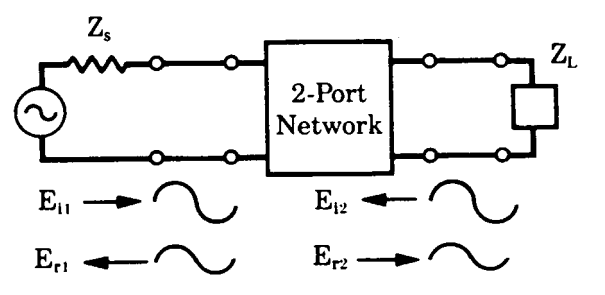
\includegraphics[width=0.6\textwidth]{bilder/s_parameters}
\caption{2-Port-Network \cite{aglient_s_parameters}}
\label{fig:2_port_network}
\end{figure}

\begin{align}
V_{1}&=h_{11}I_{1}+h_{12}V_{2}\\
I_{2}&=h_{21}I_{1}+h_{22}V_{2}
\label{eq:voltage_current}
\end{align}
Where $h_{11},h_{12},h_{21}$ and $h_{22}$ are H-Parameters and defined in (\ref{eq:h_parameters1}-\ref{eq:h_parameters2}).
\begin{align}
h_{11}&=\frac{V_{1}}{I_{1}}|_{V_{2}=0}\quad h_{12}=\frac{V_{1}}{V_{2}}|_{I_{1}=0}
\label{eq:h_parameters1}\\
h_{21}&=\frac{I_{2}}{I_{1}}|_{V_{2}=0}\quad h_{22}=\frac{I_{2}}{V_{2}}|_{I_{1}=0}
\label{eq:h_parameters2}
\end{align}
But H-Parameters cannot always be valid for the description of a circuit of microwave circuits. Agilent\cite{aglient_s_parameters} has listed some problems in high frequency:
\begin{itemize}
\item It is not easy to measure the total voltage and total current at the ports of the network.
\item Short and open circuits are not always available for a broad frequency band.
\item For high frequency some circuit are not stable in short or open conditions.
\end{itemize}
Scattering parameters or S-parameters are perfect description of microwave circuit\cite{RF194_s_parameters}. In that case traveling waves are applied instead of total voltages and currents. $E_{i1}$ and $E_{i2}$ represent incidence waves over left and right ports of the network respectively. $E_{r1}$ and $E_{r2}$ are reflective waves. The relation between traveling waves, total voltages and curents has relations (\ref{eq:voltage_wave1}-\ref{eq:voltage_wave2}).
\begin{align}
V_{1}&=E_{i1}+E_{r1}\quad V_{2}=E_{i2}+E_{r2}
\label{eq:voltage_wave1}\\
I_{1}&=\frac{E_{i1}-E_{r1}}{Z_{0}}\quad I_{2}=\frac{E_{i2}-E_{r2}}{Z_{0}}
\label{eq:voltage_wave2}
\end{align}
Traveling waves themselves can be expressed in terms of H-Parameters (\ref{eq:er1}\ref{eq:er2}). 
\begin{align}
E_{r1}&=f_{11}(h)E_{i1}+f_{12}(h)E_{i2}
\label{eq:er1}
\\
E_{r2}&=f_{21}(h)E_{i1}+f_{22}(h)E_{i2}
\label{eq:er2}
\end{align}
Here $f11, f12, f21, f22$ are the network parameters, which indicate the relation between traveling voltages waves and total voltages or currents. Divide both sides of the functions(\ref{eq:er1}-\ref{eq:er2}) by $\sqrt{Z_{0}}$( $Z_{0}$ system impedance).A new set of variables are defined:
\begin{align} 
a1&=\frac{Ei1}{\sqrt{Z_{0}}}=\frac{V_{1}+I_{1}Z_{0}}{2\sqrt{Z_{0}}} \quad a2=\frac{Ei2}{\sqrt{Z_{0}}}=\frac{V_{2}+I_{2}Z_{0}}{2\sqrt{Z_{0}}} \\
b1&=\frac{Er1}{\sqrt{Z_{0}}}=\frac{V_{1}-I_{1}Z_{0}}{2\sqrt{Z_{0}}}  \quad b2=\frac{Er2}{\sqrt{Z_{0}}}=\frac{V_{2}-I_{2}Z_{0}}{2\sqrt{Z_{0}}}
\end{align}
So relations of the new variables are give by:
\begin{align}
b_{1}&=S_{11}a_{1}+S_{12}a_{2}\\
b_{2}&=S_{21}a_{1}+S_{22}a_{2}
\end{align}
or in matrics form:
\begin{equation}
		\begin{pmatrix}
			b_{1}&\\
			b_{2}&
		\end{pmatrix}
	=	
		\begin{pmatrix}
			S_{11}&S_{12}\\
			S_{21}&S_{22}
		\end{pmatrix}
		\begin{pmatrix}
			a_{1}&\\
			a_{2}&
		\end{pmatrix}
\label{eq:s_matrix}
\end{equation}

The S-Parameters are defined as following:
\begin{align}
S_{11}&=\frac{b_{1}}{a_{1}}|_{a_{2}=0}\\
S_{21}&=\frac{b_{2}}{a_{1}}|_{a_{2}=0}\\
S_{22}&=\frac{b_{2}}{a_{2}}|_{a_{1}=0}\\
S_{12}&=\frac{b_{1}}{a_{2}}|_{a_{1}=0}
\end{align}
The phical meaning of the S-Parameters are described as following:
\begin{itemize}
\item $S_{11}$ is the input port reflection coefficient
\item $S_{12}$ is the reverse gain
\item $S_{21}$ is the forward gain
\item $S_{22}$ is the output port reflection coefficient
\end{itemize}
In another hand, $S_{21}$ is often used to estimate the transmission ability of a network. Therefore $S_{21}$ equals the coupling efficiency in this work.


\chapter{Modelling}
\label{chp:model}
%%Chapter2
%description

In this chapter the configurations of the experimental objects and corresponding technical detail will be at first introduced. Then it will be described the detail how the simulation models are approximated in CST MWS (CST Studio suite 2010) and the some performances of the simulations will also be illustrated in compare with the practical objects, such as working distance, minimum spot size, power distribution, etc .

\section{Project description}
%%%%%% Problem description
The left side is a lensed tapered fiber as laser source and at the right side at the working distance there is a chip formed waveguide as signal receiver.  The purpose is to find a way to gain optimized coupling efficiency through the simulations in CST MWS Environment (CST Studio suite 2010), which is a electromagnetic simulator basically with the implementation of the Finite Integration Technique (FIT)\cite{ cst_help_siulation_method}. 


Following is a typical demonastration of fiber-to-chip coupling.
\begin{figure}
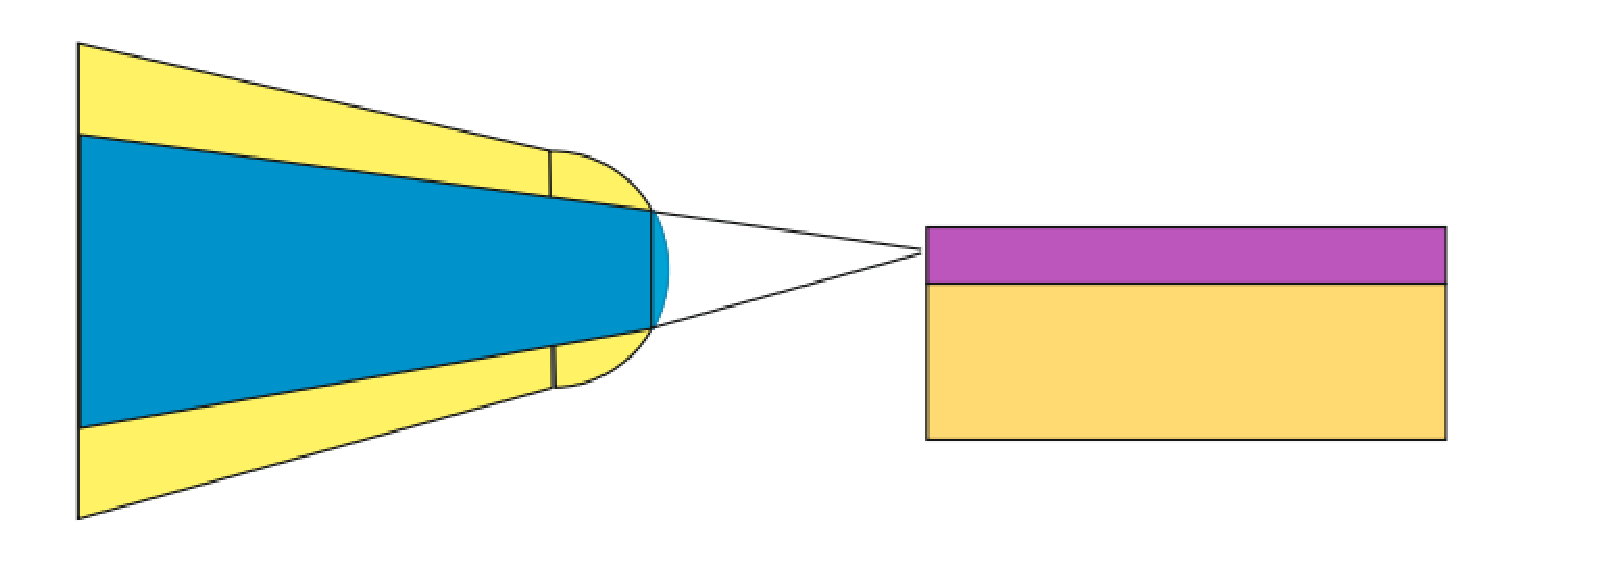
\includegraphics[width=.7\textwidth]{bilder/experiment_object}
\caption{Fiber-to-Chip Coupling}
\label{fig:experiment_object}
\end{figure}

\begin{figure}
\centering
\subfigure[Picture of a real Single mode lensed fiber\cite{nanoscal_tapered_fiber}.]{
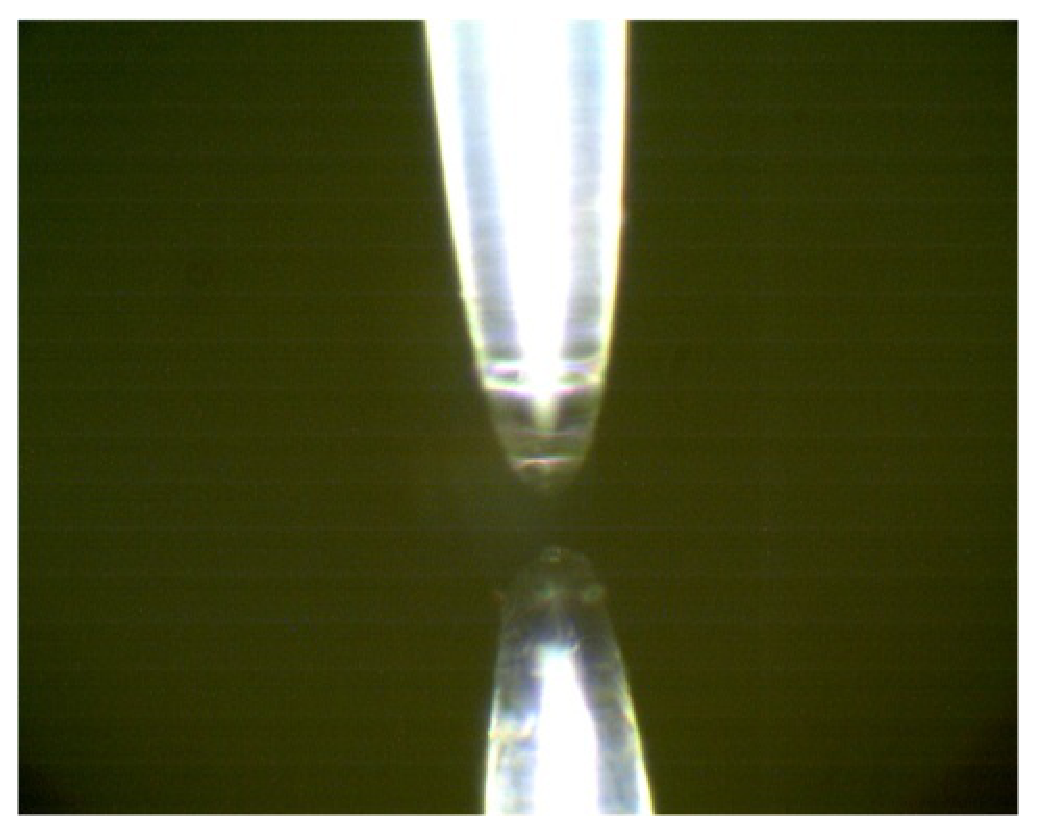
\includegraphics[width=0.3\textwidth]{bilder/single_mode_lensed_fibber}
\label{fig:single_mode_lensed_fiber}
}
\hfill
\subfigure[Schema of a tapered lensed fiber\cite{nanoscal_tapered_fiber}.]{
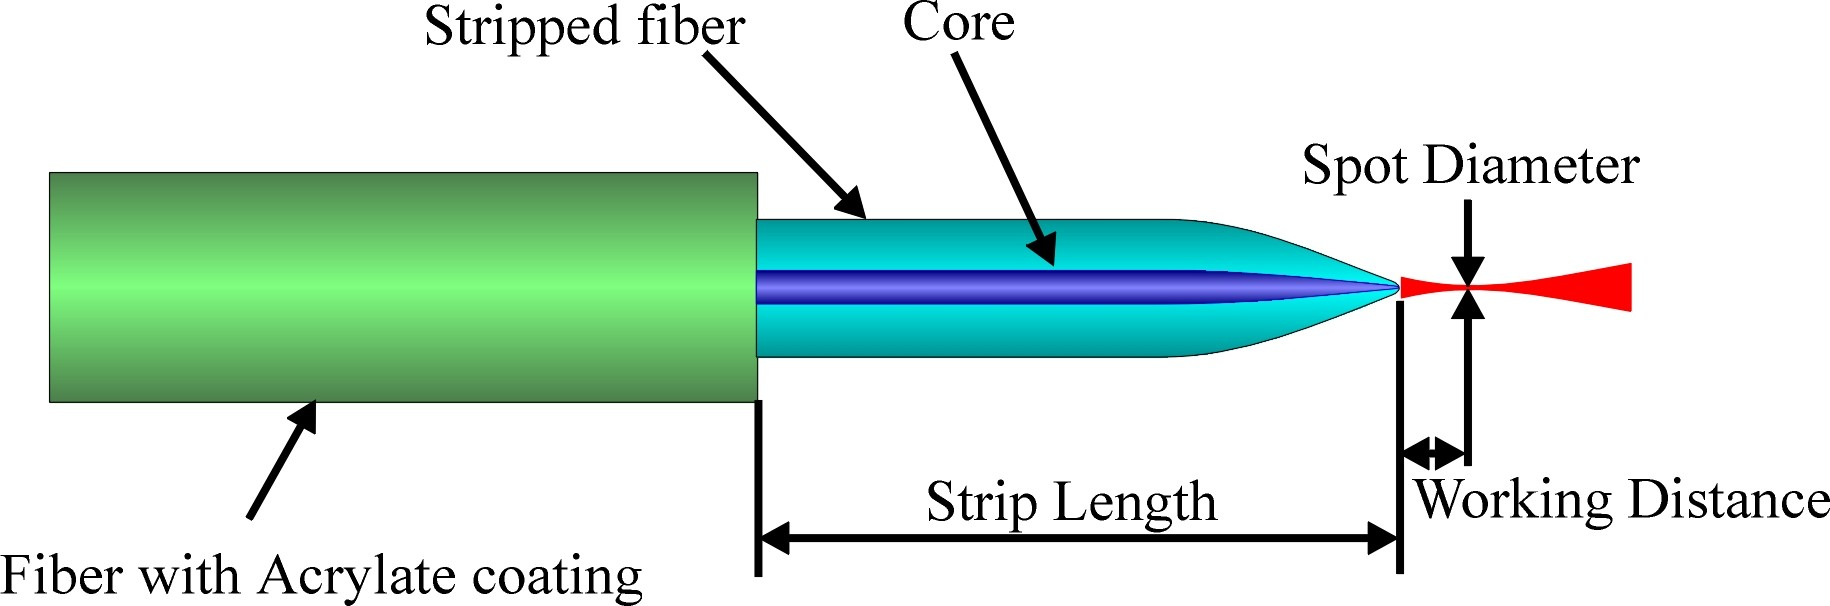
\includegraphics[width=0.6\textwidth]{bilder/tapered_lensed_fiber}
\label{fig:tapered_lensed_fiber}
}
\label{fig:TLFs}
\caption{NANOICS Tapered and Lensed Fibers}
\end{figure}


In this article the the tapered lensed fiber from \textbf{NANONICS} will be used. Fig.\ref{fig:single_mode_lensed_fiber} is the real image of the fiber and Fig.\ref{fig:tapered_lensed_fiber} indicate its schema. In Table\ref{tab:technical parameters_lensed_fiber} are listed part of technical parameters, which refer later to the modeling. Additionally the real woking frequence is $\lambda=1064nm$ and working distance but $4\mu m$. 


\begin{table}
\begin{tabular}{c|c|c}
\hline
\multicolumn{2}{c|}{\textbf{Parameter}}&\textbf{Specification(Single-Mode)}\\
\hline
\multirow{3}{*}{\parbox[t]{0.25\textwidth}{Spot Size of Aspheric and Convex Lenses($1/e^2$)}}&\multirow{2}{*}{Minum}&$1.7\mu m(\lambda=1.5\mu m)$\\
&																		 &$0.6\mu m(\lambda=0.6\mu m)$\\
&Maxium															 &$6.0\mu m(\lambda=1.5\mu m)$\\
\hline
\multirow{2}{*}{Spot Size Tolerance}&Without near-field characterization &$\pm 0.5\mu m$\\
&With near-field characterization &$\pm 0.25\mu m$\\
\hline
\multirow{2}{*}{Working Distance} &Minimum &$5\mu m(\lambda=1.5\mu m)$\\
&																	Maximum &$50\mu m(\lambda=1.5\mu m)$\\
\hline
\end {tabular}
\caption{Technical parameters about tapered lensed fiber.\cite{nanoscal_tapered_fiber}}
\label{tab:technical parameters_lensed_fiber}
\end{table}



\begin{figure}
\centering
\subfigure[Schema of a real waveguide.]{
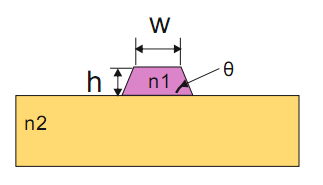
\includegraphics[width=0.4\textwidth]{bilder/orignial_waveguide}
\label{fig:orignial_waveguide}
}
\hfill
\subfigure[Schema of a approxmate waveguide.]{
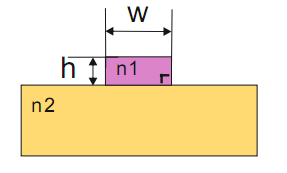
\includegraphics[width=0.4\textwidth]{bilder/approxmate_waveguide}
\label{fig:approxmate_waveguide}
}
\caption{Introduction of  photonic waveguide}
\label{fig:photonic_waveguide}
\end{figure}

The real waveguide Fig.\ref{fig:orignial_waveguide} is a trapezoid guide on a semiconductor. But the angles $\theta$ of this guide approximate to $90^{o}$ and is not easy to measure because of its micro-size. Thus a simplified guide model Fig.\ref{fig:approxmate_waveguide} will be used in this article. And the detailed technical properties of the photonic waveguide are given:
\begin{itemize}
\item working frequence $\lambda=1064 \mu m$
\item guide :$LiNbO_{3}$ with $ n1=2.516, w\approx 1\mu m, h\approx 0.5 \mu m$
\item substratum: $SiO_{2}$ with $n2=1.544 $
\end{itemize}
% arrange the name to 'project_description' 23.02
%% Problem description
Coupling single-mode fibers to waveguides with the help of microlenses is a very common setup in integrated optics \cite{integrated_optics}. Because a lensed fiber has a minimum focal length, by means of this technique simple and reliable optical systems with a small size become possible. In this work the implement of the lensed fiber-to-chip will be discussed and it coupling efficiency will be discussed.\\

\begin{figure}[!ht]
\centering
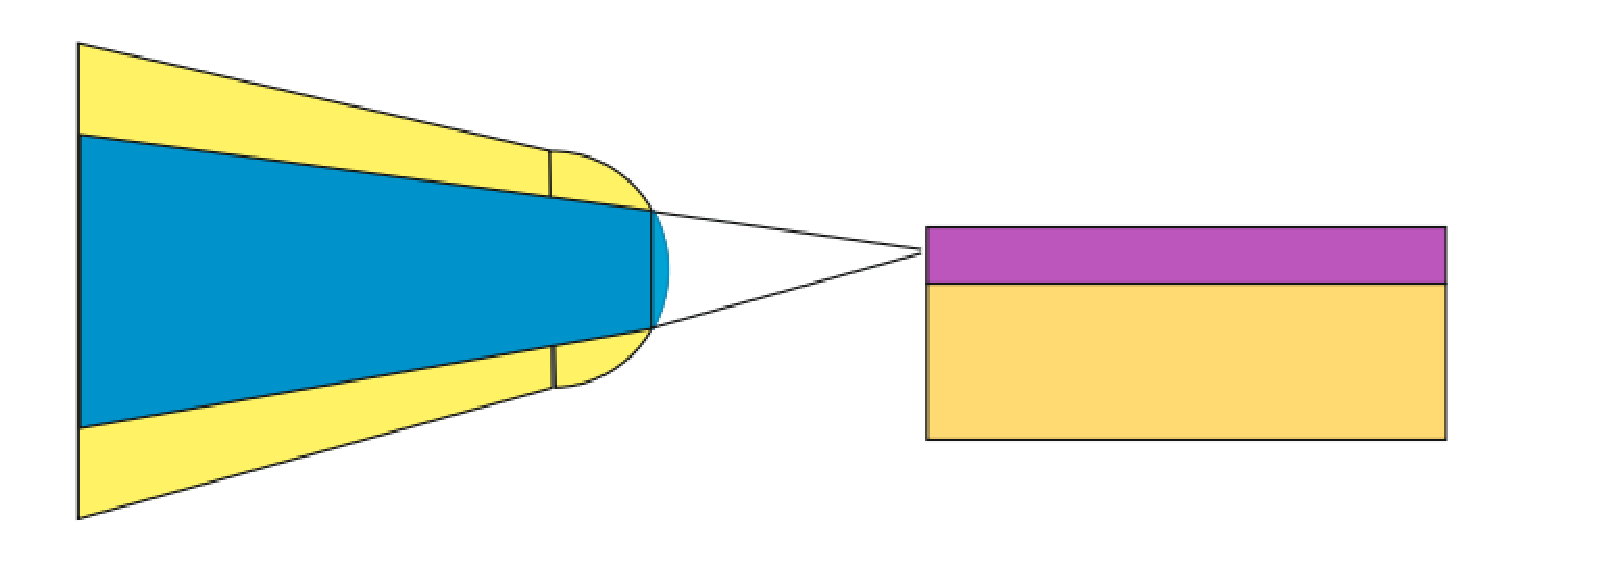
\includegraphics[width=.7\textwidth]{bilder/experiment_object}
\caption{Fiber-to-Chip interface.}
\label{fig:experiment_object}
\end{figure}
Fig. \ref{fig:experiment_object} shows a schematic fiber-to-chip interface. At the one side there is a lensed tapered fiber as laser source and at another side there is a rib waveguide\cite{integrated_optics}, located at the working distance of the fiber, as the signal receiver.\\
 
\begin{figure}[!ht]
\centering
\subfigure[Picture of a real Single mode lensed fiber\cite{nanoscal_tapered_fiber}.]{
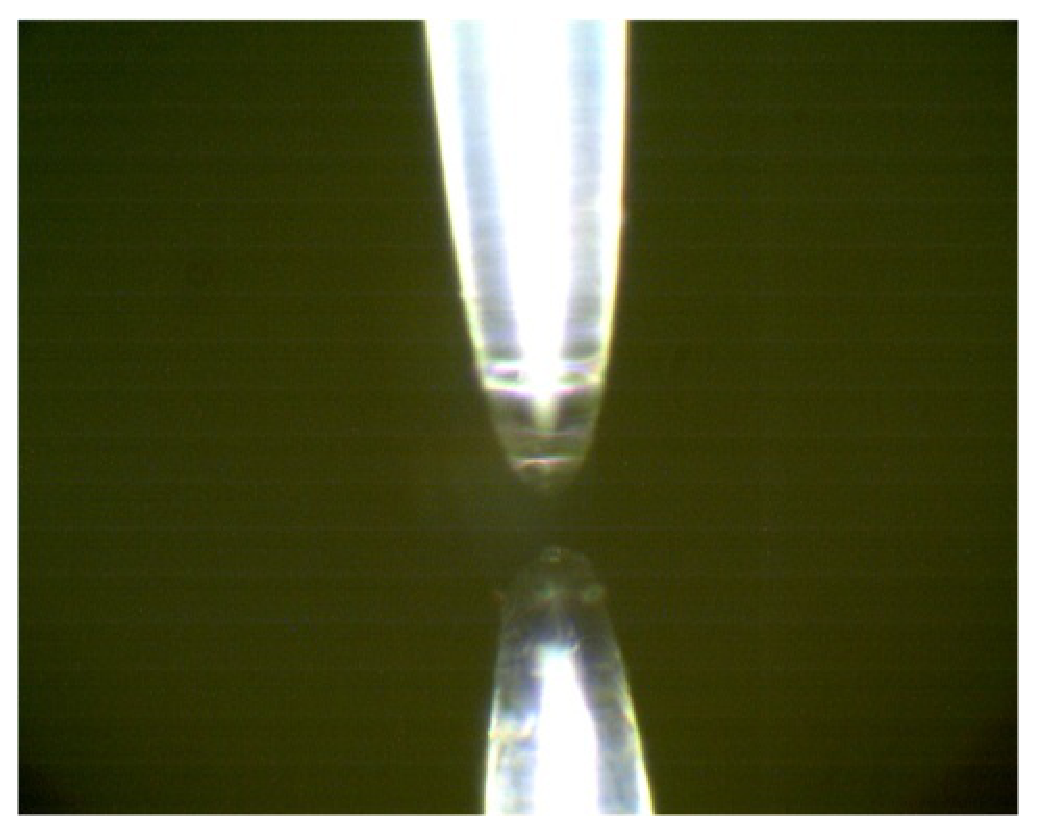
\includegraphics[width=0.3\textwidth]{bilder/single_mode_lensed_fibber}
\label{fig:single_mode_lensed_fiber}
}
\hfill
\subfigure[Schema of a tapered lensed fiber\cite{nanoscal_tapered_fiber}.]{
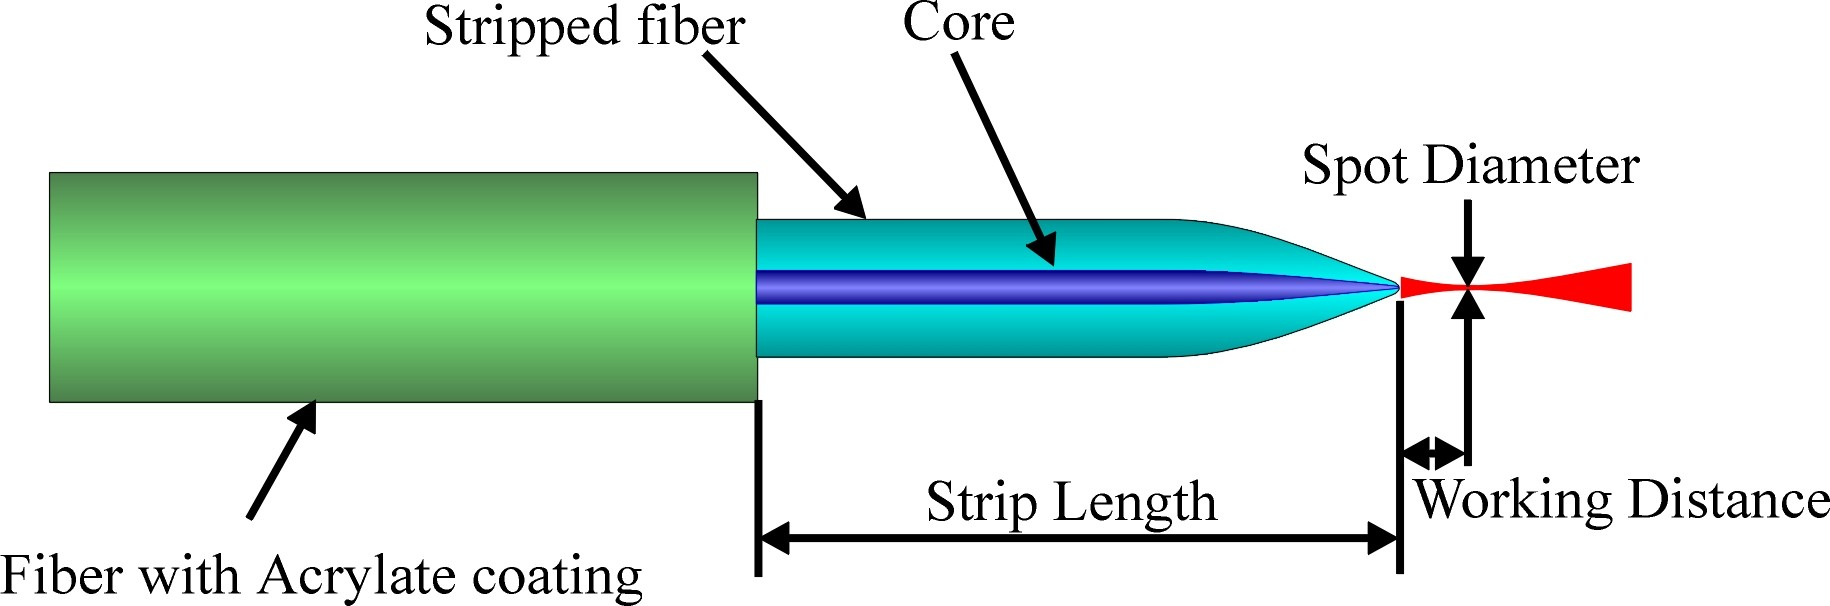
\includegraphics[width=0.6\textwidth]{bilder/tapered_lensed_fiber}
\label{fig:tapered_lensed_fiber}
}
\label{fig:TLFs}
\caption{ Tapered and Lensed Fibers by NANOICS.}
\end{figure}
In the experimental setup for this work tapered lensed fibers from NANONICS\cite{nanoscal_tapered_fiber} are used. Fig. \ref{fig:single_mode_lensed_fiber} shows the photograph of the tapered fiber by NANONICS and Fig. \ref{fig:tapered_lensed_fiber} indicate its schema. In Tab. \ref{tab:technical parameters_lensed_fiber} parts of technical parameters are listed. Additional information about the experimental setup is that the working wavelength is $\lambda=1064$nm ($f=282$THz) and working distance $4\mu$m.\\
 
\begin{table}[!ht]
\caption{Technical parameters about tapered lensed fiber\cite{nanoscal_tapered_fiber}.}
\begin{tabular}{|c|c|c|}
\hline
\multicolumn{2}{|c|}{\textbf{Parameter}}&\textbf{Specification(Single-Mode)}\\
\hline
\multirow{3}{*}{\parbox[c]{0.25\textwidth}{Spot Size of Aspheric and Convex Lenses ($1/e^2$)}
}&\multirow{2}{*}{Minum}&$1.7\mu$m($\lambda=1.5\mu$m)\\
&																		 &$0.6\mu$m($\lambda=0.6\mu$m)\\
\cline{2-3}
&Maxium															 &$6.0\mu$m($\lambda=1.5\mu$m)\\
\hline
\multirow{2}{*}{Spot Size Tolerance}&\parbox[c]{0.25\textwidth}{
\begin{center}
Without near-field characterization
\end{center}
} & $\pm 0.5\mu$m\\
\cline{2-3}
&\parbox[c]{0.25\textwidth}{
\begin{center}
With near-field characterization
\end{center}
} &$ \pm 0.25\mu$m\\
\hline
\multirow{2}{*}{Working Distance} &Minimum &$5\mu$ m($\lambda=1.5\mu$m)\\
\cline{2-3}
&																	Maximum &$50\mu$ m($\lambda=1.5\mu$m)\\
\hline
\end {tabular}
\label{tab:technical parameters_lensed_fiber}
\end{table}

\begin{figure}[!ht]
\centering
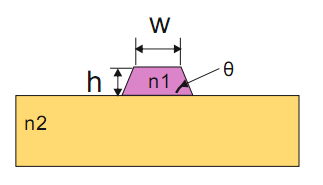
\includegraphics[width=0.6\textwidth]{bilder/orignial_waveguide}
\caption{Schema of the photonic waveguide.}
\label{fig:photonic_waveguide}
\end{figure}
Actually, the waveguide in experimental setup is a trapezoid guide on a semiconductor like Fig. \ref{fig:photonic_waveguide}. The angles $\theta$ of this guide approximate to $90^{o}$ and is not easy to measure because of the micro-size of the structure. Thus a simplified guide model with $\theta=90^{o}$ will be used in this work. The detailed technical properties of the photonic waveguide used in the experimental setup are given as following:
\begin{itemize}
\item Working wavelength: $\lambda=1064$nm
\item Waveguide: LiNbO$_{3}$ with $n_{1}=2.516, w\approx 1\mu$m, $h\approx 0.5 \mu$m
\item Substrate: SiO$_{2}$ with $n_{2}=1.544 $
\end{itemize}

\section{Modelling and Simulation}
%%modeling_introduction
For an economic simulation there is no need to create exactly identical models.  Sometimes only parts of the specifics are requested. In this section the modeling process will be discussed. 
\subsection{Modeling the Lensed Fiber}
\label{sect:model_model_model_TLF}
%%fiber_modeling

%fiber_modeling.tex
First agenda is to determine the Tapered and Lensed Fiber (TLF) model. Because of the heave computing cost creating a full size fiber is not economical. Therefore only the end of the fiber, which provides approximately the equal technical properties, will be modeled in this works.  In \cite{TLF_analysis,TLF_mode_transforming} two type of the TLF configuration are mentioned. 


\begin{figure}[!ht]
\centering
\subfigure[Tapered cladding TLF.]{
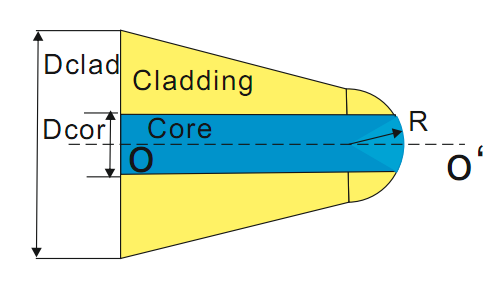
\includegraphics[width=0.4\textwidth]{bilder/lense_fiber_01}
\label{fig:lense_fiber_01}
}
\hfill
\subfigure[Tapered core TLF.]{
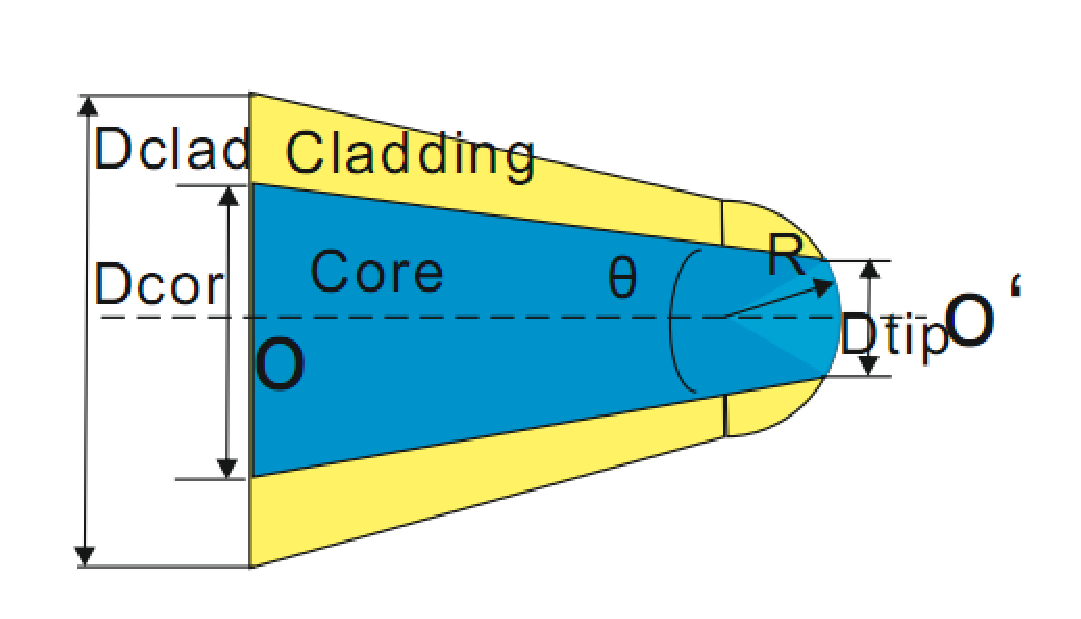
\includegraphics[width=0.4\textwidth]{bilder/lense_fiber_02}
\label{fig:lense_fiber_02}
}
\label{fig:two_TLF}
\caption{Two types of Tapered and Lensed Fibers}
\end{figure}

The tapered cladding TLF Fig.\quad\ref{fig:lense_fiber_01} shows that its cladding diameter decreases along the beam propagation direction (O-O'Axis) and its core diameter is a constant. For the tapered core TLF Fig.\quad\ref{fig:lense_fiber_02} its cladding diameter and core diameter both decrease along the axis. In \cite{TLF_mode_transforming} the Authour tried to develop methods to estimate the performance of both type of TLF. His results show that the performance of the first type of TLF agrees well with the estimation and that of the second type is unpredictable. In this section two TLF models from each type are created and their performances are tested in CST MWS.  
First of all, determination the lens of both types is primary. For simplification, a hemispherical lens is assumed at the end of the fiber. Considering the working distance of the practical TLF, the lens configuration can be estimated through the lens theory. After estimations and some simulations one configuration of the lens is carefully selected Tab.\quad\ref{tab:model_fiber_configuration}.   

\begin{table}
\caption{Configurations of the TLF Models}
\centering
\begin{tabular}{ccc}
\hline
							&Tapered Cladding&Tapered Core\\
\hline
R($\mu$m) & $6$						 &$6$	\\
n$_{core}$&$1.68$&$1.68$\\
n$_{cladding}$&$1.66$&$1.66$\\
D$_{clad}$($\mu$m) &	$17$ &	$17$\\
D$_{core}$($\mu$m) & $10$ &	$17$\\
D$_{tip}$ ($\mu$m) & --   &	$6$\\
\hline
\end{tabular}
\label{tab:model_fiber_configuration}
\end{table}
From Fig.\quad\ref{fig:lens_spot} the beam propagation is demonstrated base on lens theory. As is in previous chapter described, the minimum spot located not exactly at the focal length. From measures of the location of Paraxial focal plane(PP) and that of meridional plane (MP) the minimum spot(MS) can be estimated. In the above configuration the theoretical distance from lens end to PP is $8.82 \mu$ m and the distance from lens end to MP is about $2.74 \mu$m. Backword $3/4$ longitudinal spherical aberration(LAm) form PP, the MS is founded at the place about $4.26 \mu$m far from lens end. 
\begin{figure}[!ht]
\centering
	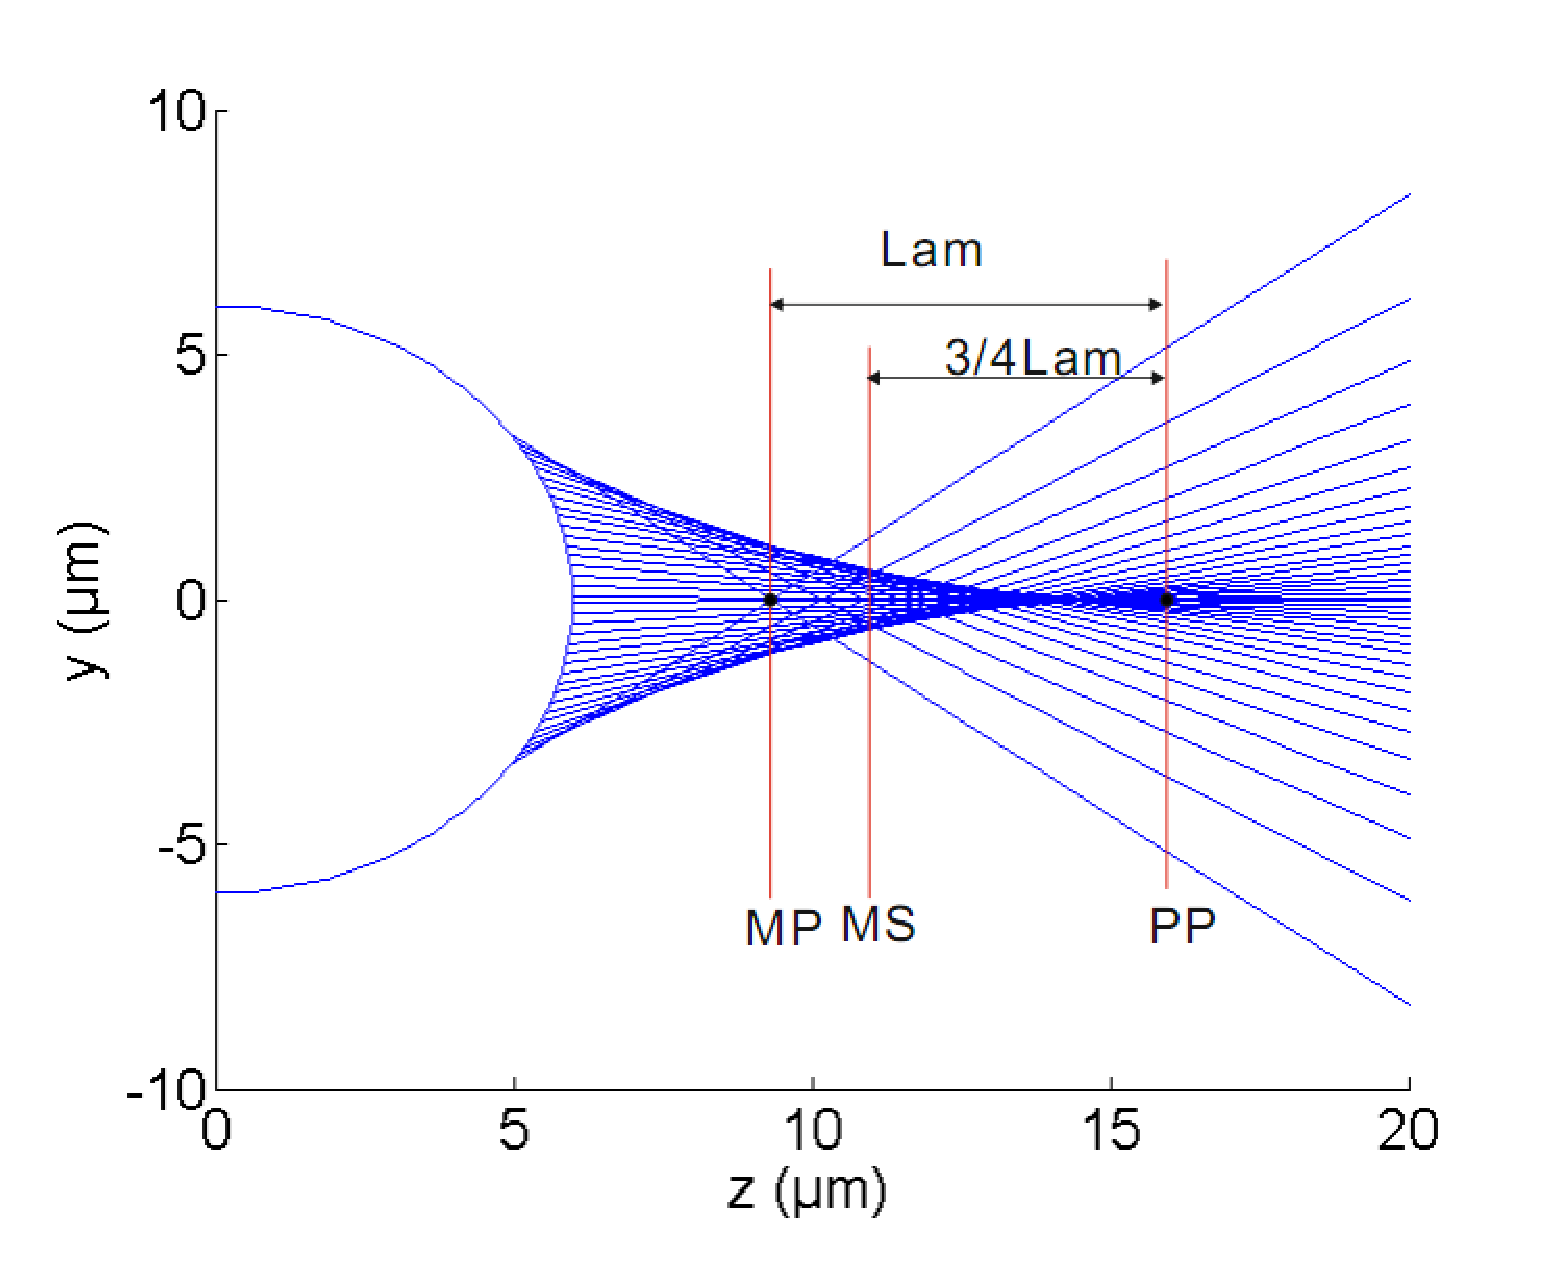
\includegraphics[width=0.7\textwidth]{bilder/cal_min_spot}
\caption{Beam Propogation from lense.}
\label{fig:lens_spot}
\end{figure}
Implement this configuration for both types of TLF models in CST. Through simulations, E-Field demonstrations in the xz-plane of both types of TLFs can be drown as Fig. \ref{fig:Tapered_cladding_efield} and  Fig. \ref{fig:Tapered_core_efield}, wich have no great difference.
\begin{figure}[!ht]
	\centering
		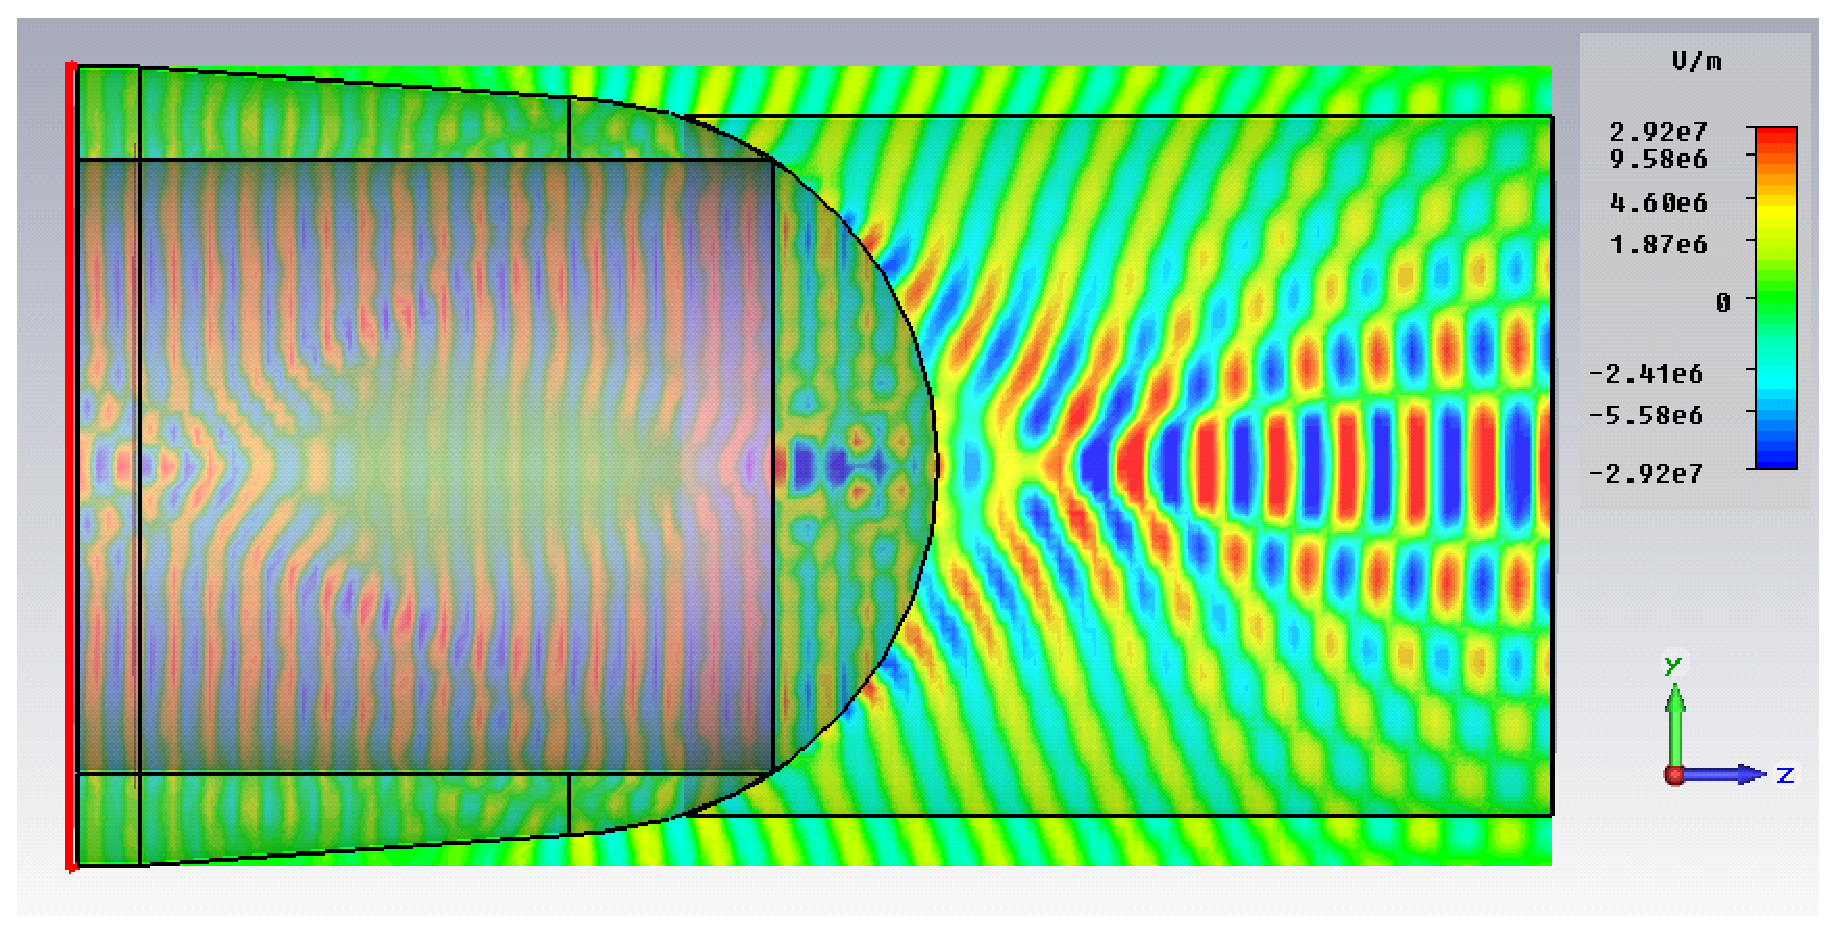
\includegraphics[width=0.8 \textwidth]{bilder/cst_lensed_fiber_equ_efield}
		\caption{E-Field demonstration of Tapered cladding TLF}
 		\label{fig:Tapered_cladding_efield}
\end{figure}

\begin{figure}[!ht]
	\centering
		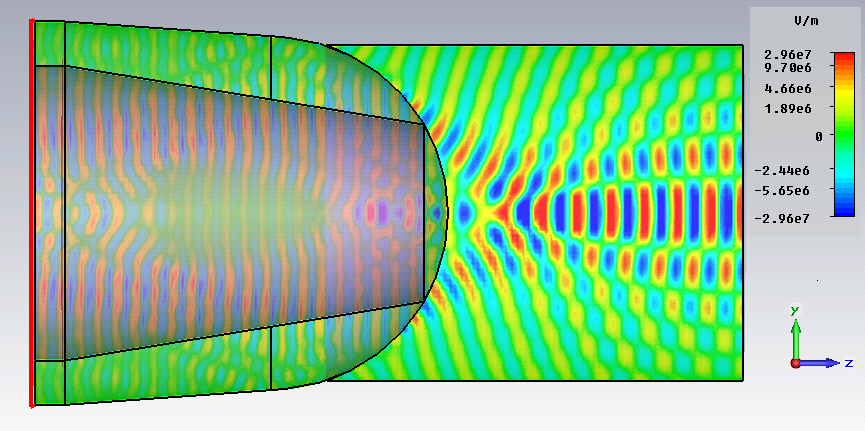
\includegraphics[width=0.8 \textwidth]{bilder/cst_lensed_fiber_efield}
		\caption{E-Field demonstration of Tapered core TLF}
 		\label{fig:Tapered_core_efield}	
\end{figure}
Load the its beam propagation detail into Matlab workspace and draw
Fig.\ref{fig:Tapered_cladding_spot_curve} and Fig.\ref{fig:Tapered_core_spot_curve},which shows the beam spot diameters through their absolute beam power flow densities or its z-compents(propagation direction) along the propagation distance. From these two figures, curves of the absolute value of their power flow density are more obvious to help people to find the minimum spot of lenses. In Fig.\ref{fig:Tapered_cladding_spot_curve} that the minimum spot size locate at about $4.1 \mu m$ from lense end and spot size equal about $1.5 \mu m$. While in Fig.\ref{fig:Tapered_core_spot_curve} that the minimum spot size is found at  $4.3 \mu m$ from lense end and spot size equal about $1.5 \mu m$. Thus it is concluded that two configuration has only a small difference. By rechecking the properties in Tab.\ref{tab:technical parameters_lensed_fiber} both TLF model are acceptable for the following development. In this works the tapered core TLF will be used for further simulations.
Fig.\ref{fig:Tapered_cladding_spot_curve}-\ref{fig:Tapered_core_spot_curve} to illustrate the beam Spot size diameter along the longitude axis.
\begin{figure}[!ht]
		\centering
		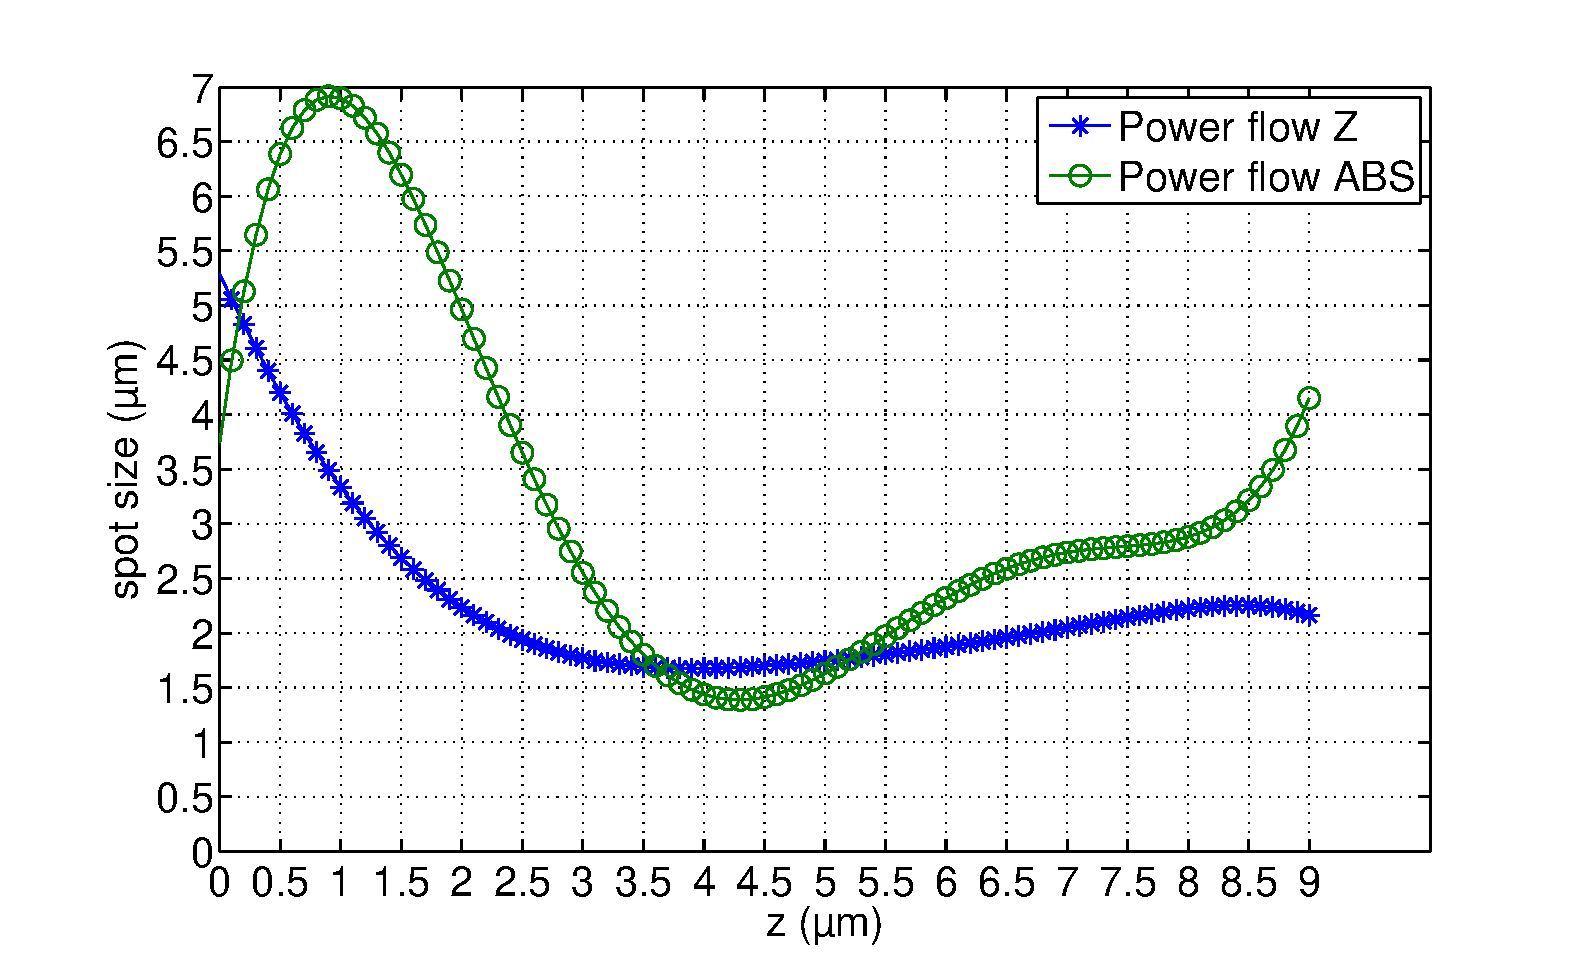
\includegraphics[width=0.7 \textwidth]{bilder/Tapered_cladding_spot_curve}
		\caption{Spot Size Curve of Tapered cladding TLF}
		\label{fig:Tapered_cladding_spot_curve}
\end{figure} 
\begin{figure}[!ht]
		\centering
		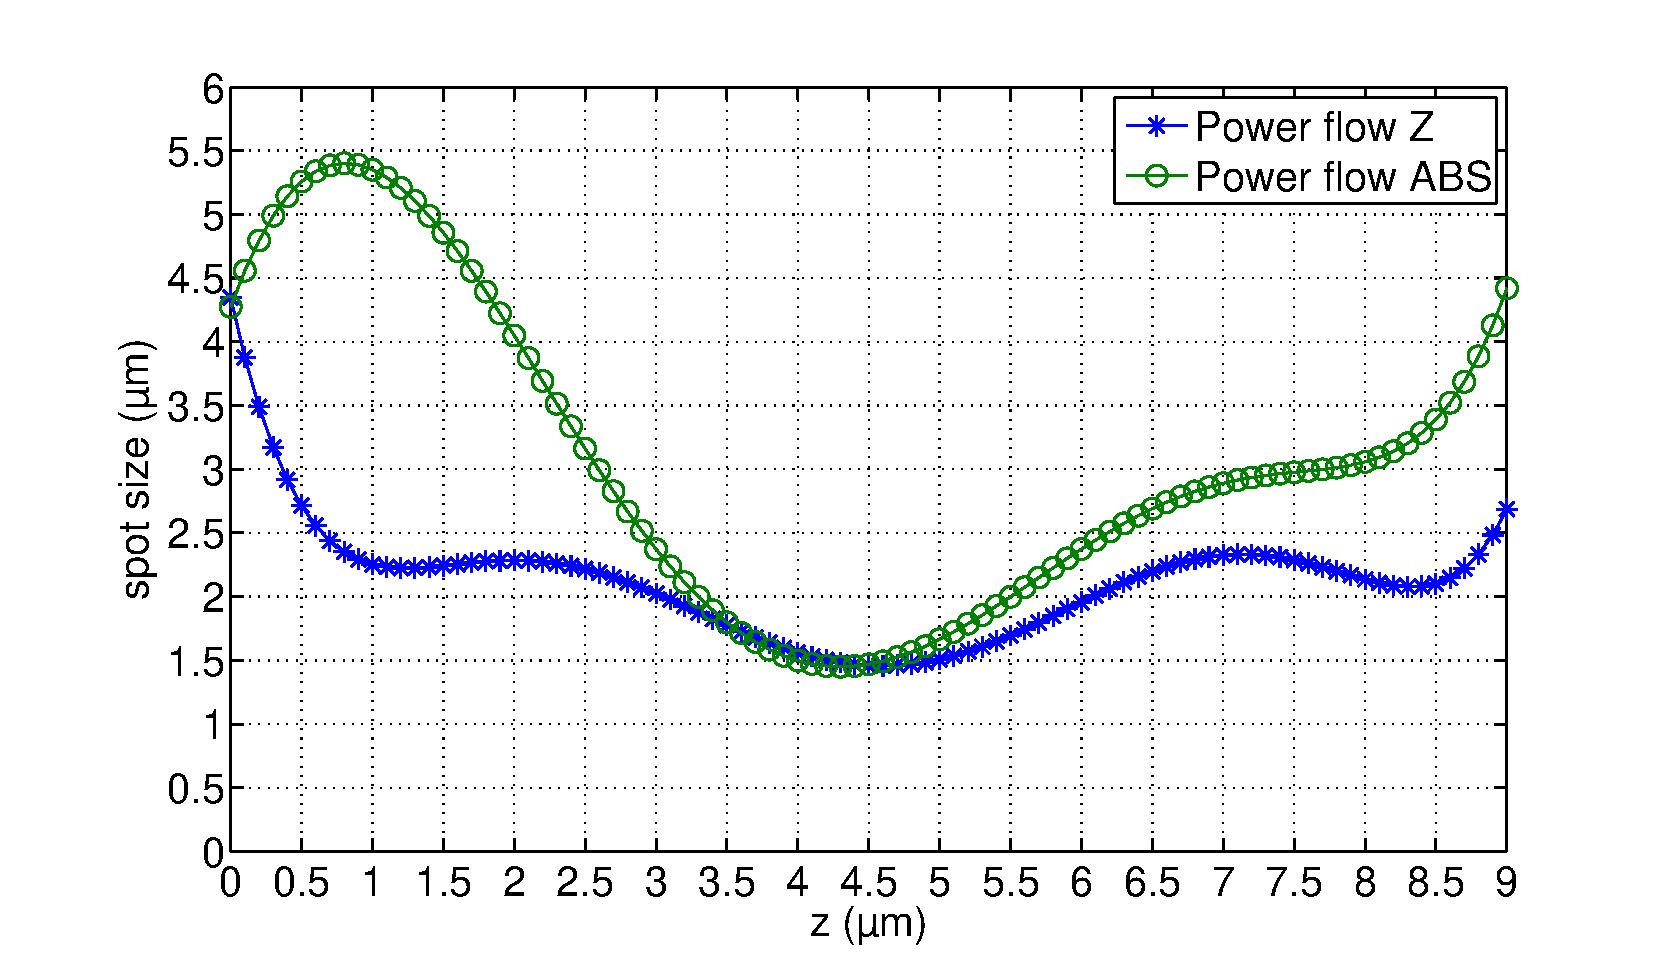
\includegraphics[width=0.7 \textwidth]{bilder/Tapered_core_spot_curve}
		\caption{Spot Size Curve of Tapered core TLF}
 		\label{fig:Tapered_core_spot_curve}	
\end{figure}

For a clear view of the beam propagation from the tapered core TLF, 3D Fig.\quad\ref{fig:3d_spot_sub1}-\ref{fig:3d_spot_sub8} of beam power densities at different distances are demonstrated. It is obvious that the power density of the beam center rise firstly along the distance and at $4\mu$m reach the hightest value. Then it falls slowly. This tendency agrees with its spot size curve inversely. 
\begin{figure}[!ht]
\setlength{\abovecaptionskip}{0pt}% 
\flushleft
	\subfigure[3D Beam Power at distance $1\mu m$]{
	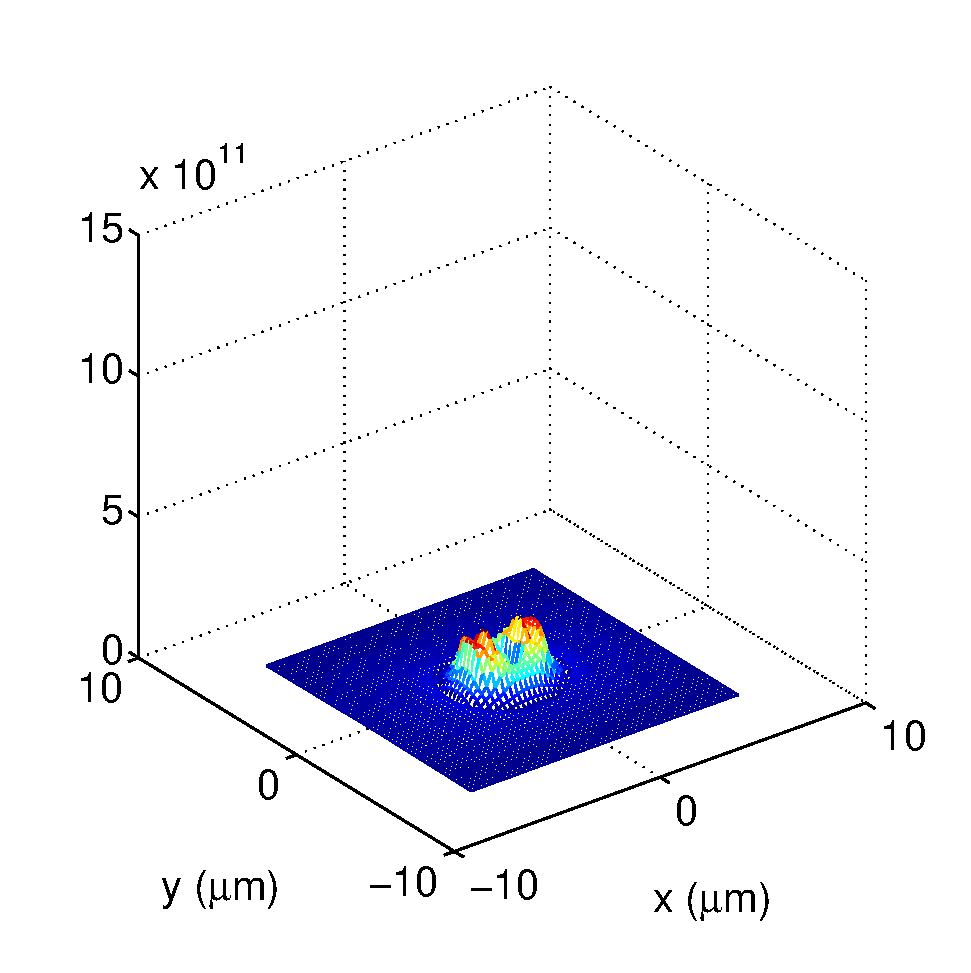
\includegraphics[width=0.4 \textwidth]{bilder/surf_spot_1um}
	\label{fig:3d_spot_sub1}%
	}
 	\subfigure[3D Beam Power at distance $2\mu m$]{
 	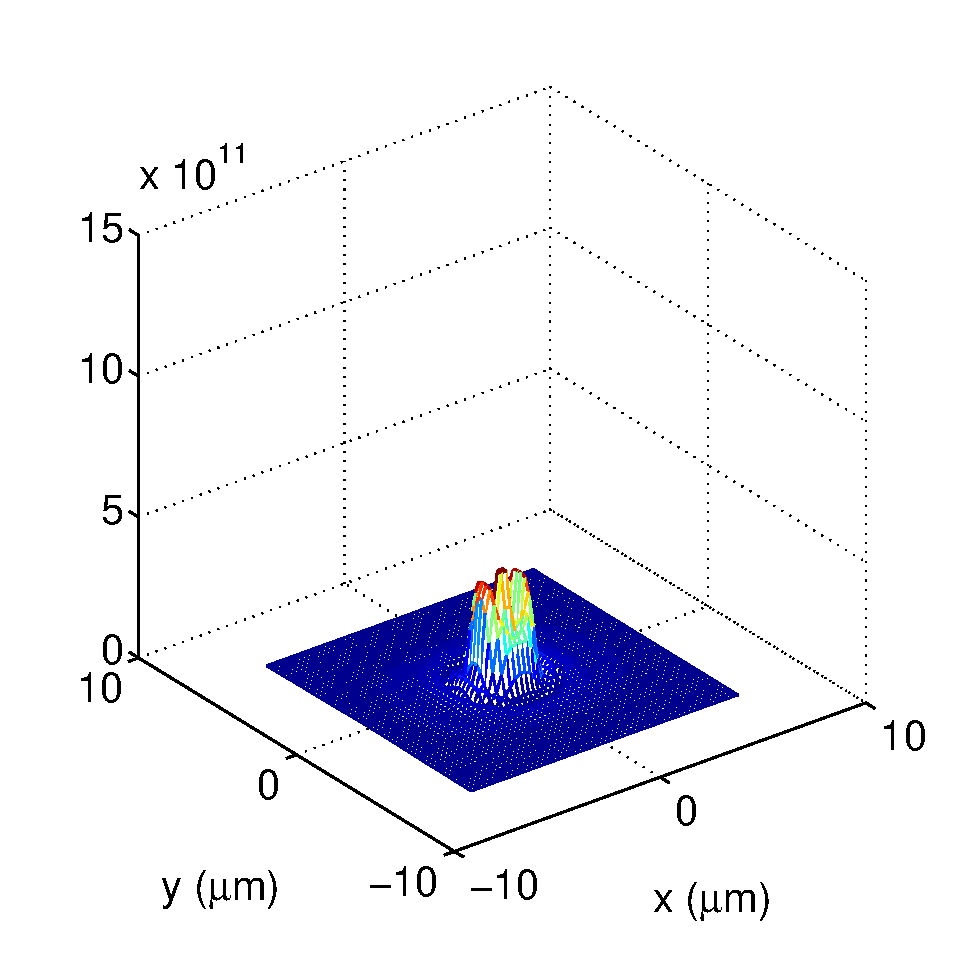
\includegraphics[width=0.4 \textwidth]{bilder/surf_spot_2um}
 	\label{fig:3d_spot_sub2}
 	}
\end{figure}	
\begin{figure}[!ht]
\setlength{\abovecaptionskip}{0pt}% 
\flushleft
 	 	\subfigure[3D Beam Power at distance $3\mu m$]{
 	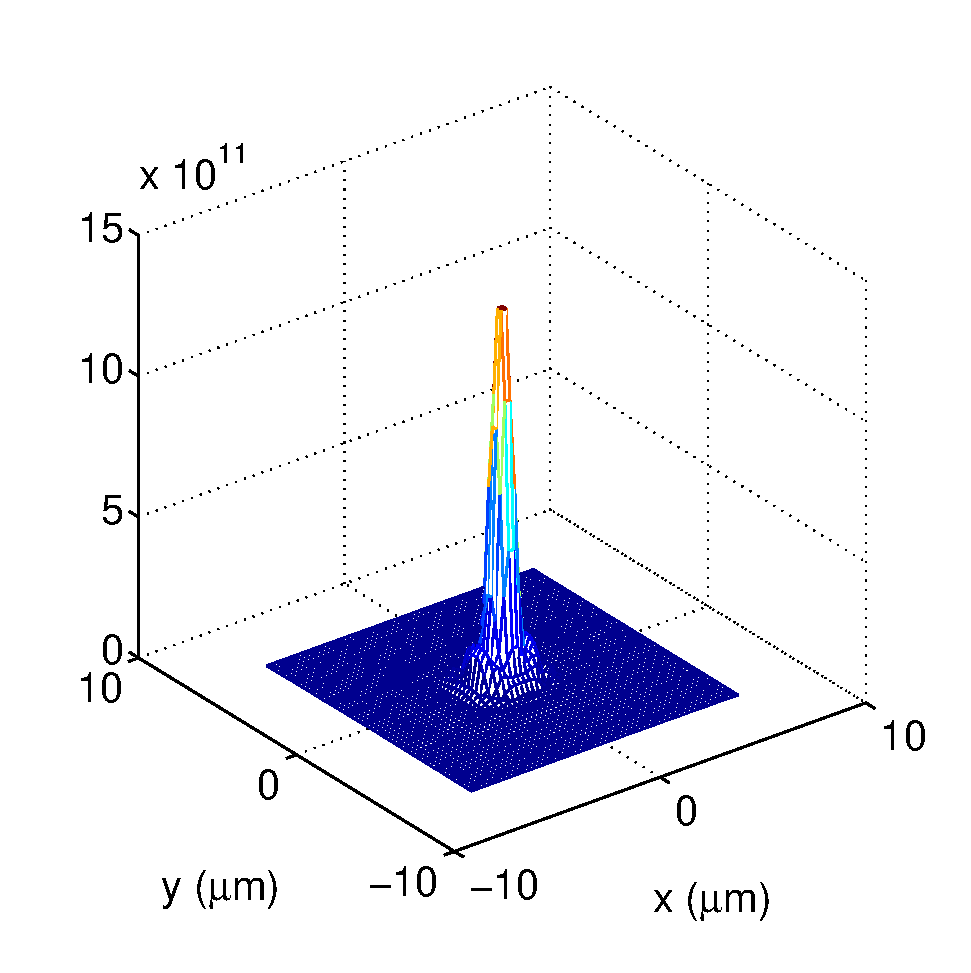
\includegraphics[width=0.4 \textwidth]{bilder/surf_spot_3um}
 	\label{fig:3d_spot_sub3}
 	}
 	\subfigure[3D Beam Power at distance $4\mu m$]{
 	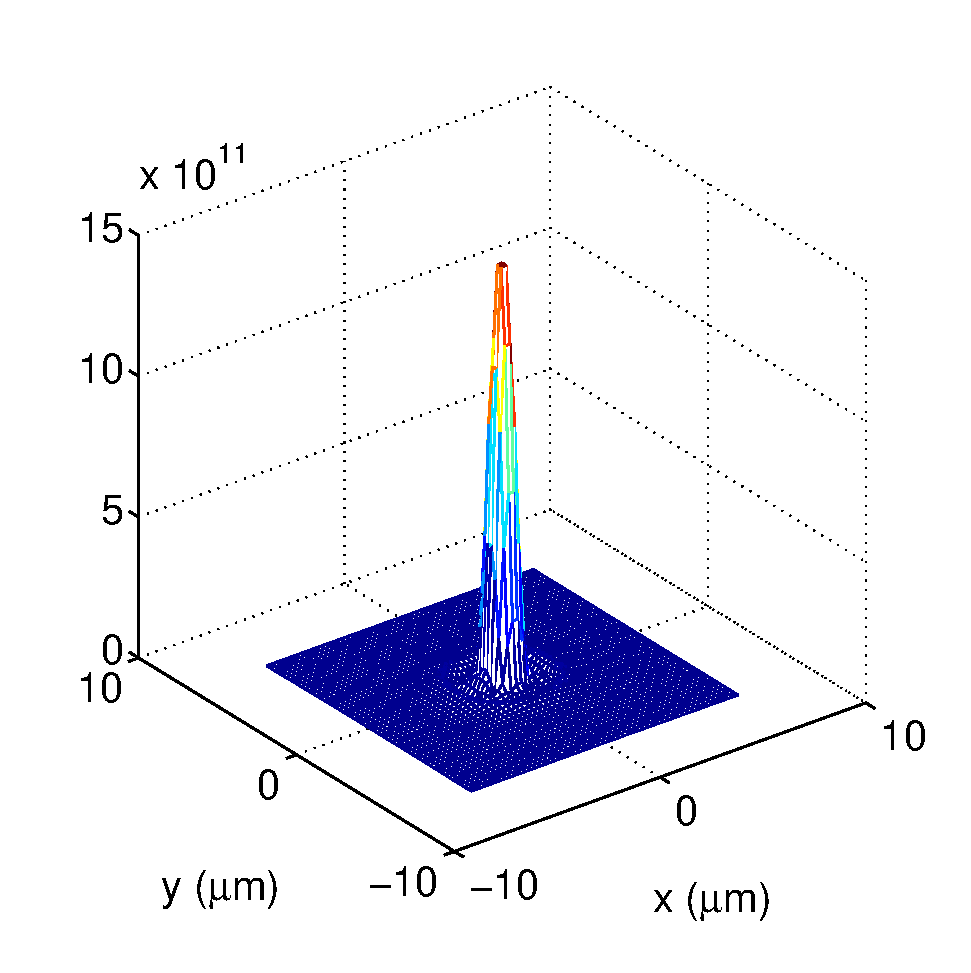
\includegraphics[width=0.4 \textwidth]{bilder/surf_spot_4um}
 	\label{fig:3d_spot_sub4}
 	}
\end{figure}	
\begin{figure}[!ht]
\setlength{\abovecaptionskip}{0pt}% 
\flushleft
 	 \subfigure[3D Beam Power at distance $5\mu m$]{
 	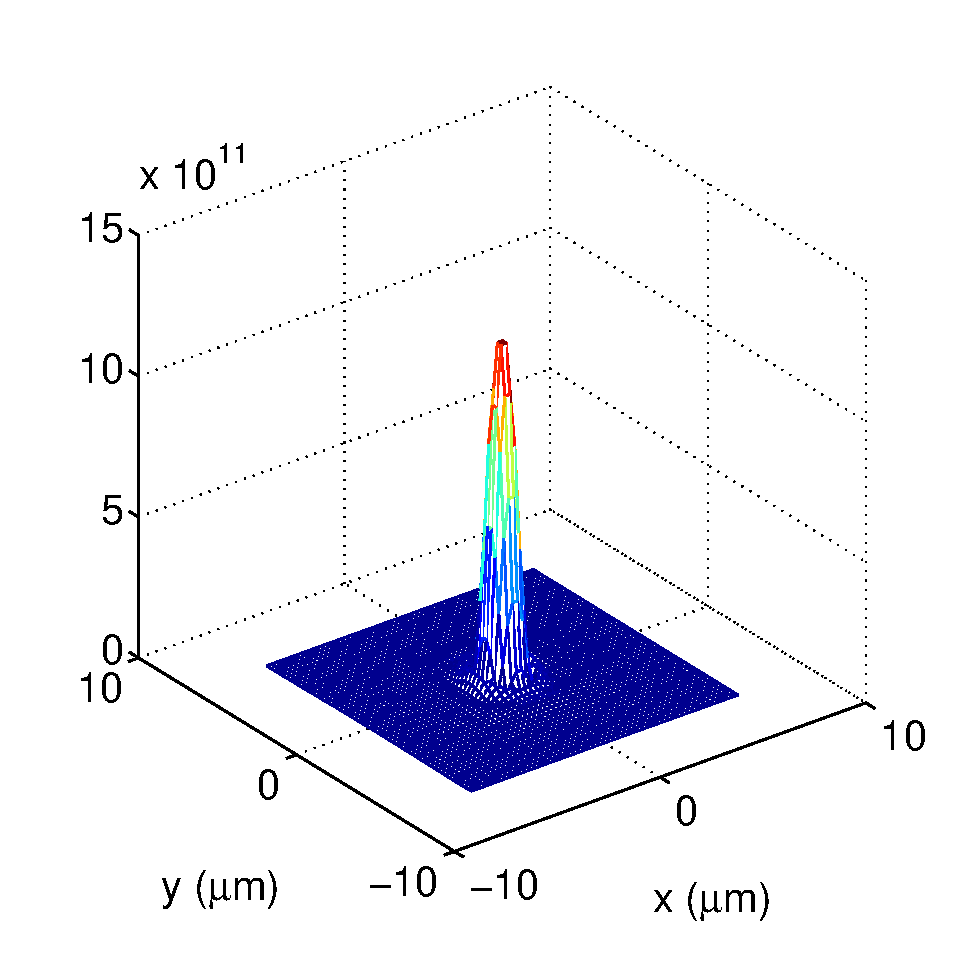
\includegraphics[width=0.4 \textwidth]{bilder/surf_spot_5um}
 	\label{fig:3d_spot_sub5}
 	}
 	 	\subfigure[3D Beam Power at distance $6\mu m$]{
 	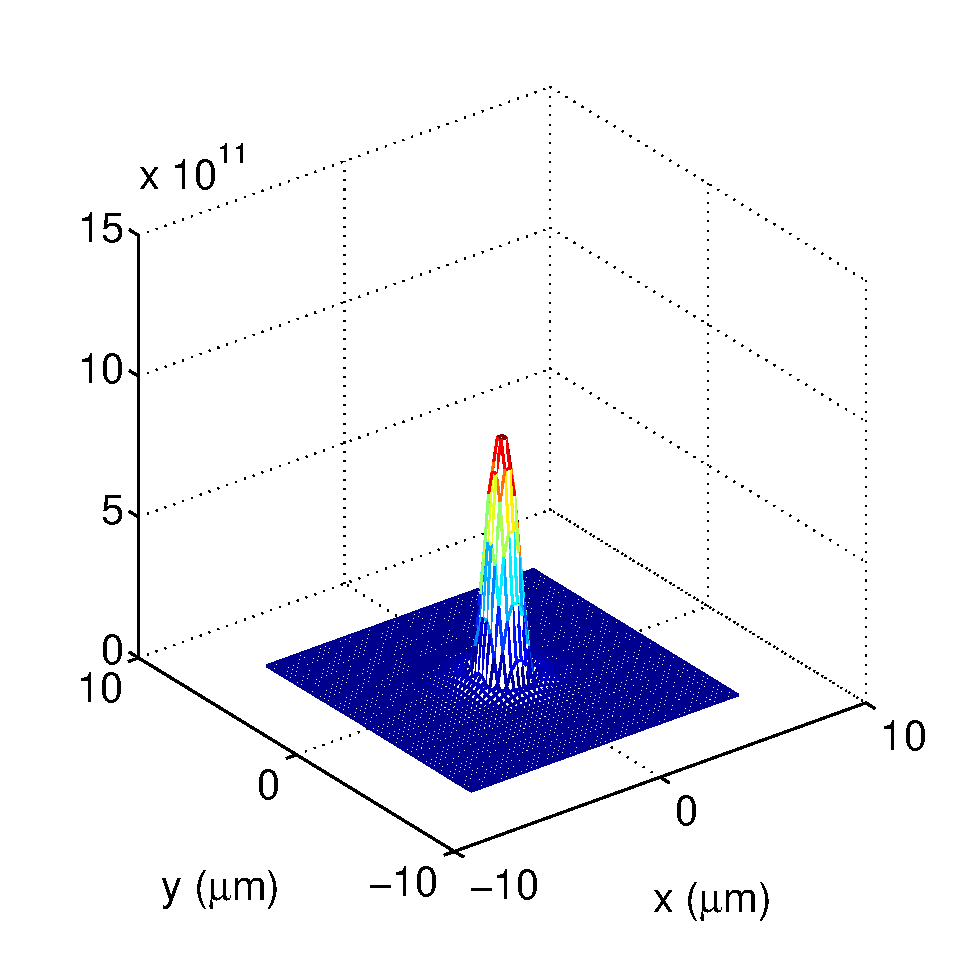
\includegraphics[width=0.4 \textwidth]{bilder/surf_spot_6um}
 	\label{fig:3d_spot_sub6}
 	}
\end{figure}	
\begin{figure}[!htp]
\setlength{\abovecaptionskip}{0pt}% 
\flushleft
  \subfigure[3D Beam Power at distance $7\mu m$]{
 	\includegraphics[width=0.4 \textwidth]{bilder/surf_spot_7um}
 	\label{fig:3d_spot_sub7}
 	}
 	\subfigure[3D Beam Power at distance $8\mu m$]{
 	\includegraphics[width=0.4 \textwidth]{bilder/surf_spot_8um}
 	\label{fig:3d_spot_sub8}
 	}
 	\caption{3D Beam Power }
\end{figure} 

\subsection{Modeling the Fiber to Chip}
\label{sect:model_model_fiber2chip}
%%fiber2chip_modelings
As beginning of this chapter the waveguide model will be approximate with a rectangle waveguide. Place the waveguide at the working distance $4\mu$m before the TLF.  Fig.\quad\ref{fig:coupling_e_field} from the simulation of this configuration shows the E-Field spread more widely at the interface of the waveguide than that in the case without blockage of the waveguide and apparently a great part of E-Field infiltrate into the waveguide rather than accepted by guide. Thus by checking the S-parameter of this simulation Fig.\ref{fig:orignial_coupling_efficiency},which present the S21 in frequencies, the coupling efficiency ($S_{21}$) is about $48.8\%$ at the working frequency $282$HZ($\lambda=1064$nm). This result will act as the reference sample for the other simulations. 
\begin{figure}[!ht]
\centering
	\includegraphics[width=0.7 \textwidth]{bilder/cst_basic_waveguide_efield}
	\label{fig:coupling_e_field}
	\caption{E-Field demonstration by coupling.}
\end{figure}
Furthermore people can analyze the power distribution at the guide from Fig.\quad\ref{fig:power_distribution}( see Appendix.\quad\ref{app:powwer_distribution} ). In the figure it can be found that about $40\%$ power propagates in the guide while another $40\%$ in the substrate and the rest is losing in the air or reflecting.
\begin{figure}
\centering
\includegraphics[width=0.7\textwidth]{bilder/original_coupling_efficiency}
\caption{coupling efficiency in Frequency area.}
\label{fig:orignial_coupling_efficiency}
\end{figure}
\begin{figure}[!ht]
\centering
\includegraphics[width=0.7\textwidth]{bilder/power_distribution1}
\caption{power distribution along the waveguide.}
\label{fig:power_distribution}
\end{figure}


%
\chapter{Optimize}
\label{chp:optim}
%%optimize_introduction
This chapter aims to discuss the optimize methods so that the Fiber-to-Chip coupling efficiency improved. Four ideals are engaged in this chapter. One thought is to relocate the waveguide; another is to change the round condition of the coupling. The application of a taper interface at the beginning of the waveguide is involved in the next consideration. The last thought is to mount a lens at the waveguide interface.


\section{Coupling by location shifting}
\label{sect:optim_shift}
%%\section{Coupling by location shifting}
%coupling_shifting
As a 3D model the waveguide can be shifted on transverse (Fig. \ref{fig:shift_x_axis} and Fig. \ref{fig:shift_y_axis}) or longitude (Fig. \ref{fig:shift_z_axis}) directions.
\begin{itemize}
\item Shift the waveguide along X-Axis: Relocate the waveguide from $-0.5\mu$m to $0.5\mu$m:
\begin{figure}[!ht]
\centering
\includegraphics[width=0.7\textwidth]{bilder/shift_x_axis}
\caption{Displacing the waveguide along x-axis}
\label{fig:shift_x_axis}
\end{figure}
\item Shift the waveguide along Y-Axis: Relocate the waveguide from $-0.5\mu$m to $0.5\mu$m:
\begin{figure}[!ht]
\centering
\includegraphics[width=0.7\textwidth]{bilder/shift_y_axis}
\caption{Displacing the waveguide along y-axis}
\label{fig:shift_y_axis}
\end{figure}
\item Shift the waveguide along Z-Axis: Relocate the waveguide from $-0.5\mu$m to $0.5\mu$m:
\begin{figure}[!ht]
\centering
\includegraphics[width=0.7\textwidth]{bilder/shift_z_axis}
\caption{Displacing the waveguide along z-axis}
\label{fig:shift_z_axis}
\end{figure}
\end{itemize}

Performe above arrengments and record their simulation results $|S21|$ in Tab. \ref{tab:shift_result}:
%\begin{figure}[!ht]
%\centering
%\includegraphics[width=0.6\textwidth]{bilder/shift_curve}
%\caption{Coupling efficiency due to the displacement the waveguide along x-axis}
%\label{fig:efficiency_shift_x_axis}
%\end{figure}
%
%Shift the waveguide along Y-Axis: Relocate the waveguide from $-0.4\mu$m to $0.4\mu$m and record their forward gain $S21$:
%\begin{figure}[!ht]
%\centering
%%\includegraphics[width=0.6\textwidth]{bilder/ }
%\caption{Coupling efficiency due to the displacement the waveguide along y-axis}
%\label{fig:efficiency_shift_y_axis}
%\end{figure}
%
%Shift the waveguide along Z-Axis: Relocate the waveguide from $-0.4\mu$m to $0.4\mu$m and record their forward gain $S21$: 
%\begin{figure}[!ht]
%\centering
%%\includegraphics[width=0.6\textwidth]{bilder/ }
%\caption{Coupling efficiency due to the displacement the waveguide along z-axis}
%\label{fig:efficiency_shift_z_axis}
%\end{figure}

\begin{table}
\caption{Coupling efficiency by shifting the waveguide along X,Y and Z-Axis}
\centering
\begin{tabular}{c|c|ccc}
\hline
	\multicolumn{2}{c}{} & X-Asis & Y-Axis & Z-Axis \\
\hline
\multirow{11}{*}{\parbox[t]{0.1\textwidth}{shift distance}}&$-0.5\mu$m 		&$32.4\%$	&$32.4\%$&$46.6\%$	\\
&$-0.4\mu$m		&$37.3\%$	&$36.5\%$&$47\%$	\\
&$-0.3\mu$m 		&$41.9\%$	&$41.3\%$&$48.2\%$	\\
&$-0.2\mu$m	  &$45.5\%$	&$45.2\%$&$49.1\%$	\\
&$-0.1\mu$m		&$48\%$	&$47.8\%$&$49.1\%$	\\
&$0\mu$m			  &$48.9\%$	&$48.9\%$&$48.9\%$	\\
&$0.1\mu$m			&$47.8\%$	&$48.4\%$&$48.9\%$	\\
&$0.2\mu$m			&$45.5\%$	&$46.4\%$&$49.4\%$	\\
&$0.3\mu$m			&$41.9\%$	&$42.9\%$&$49.7\%$	\\
&$0.4\mu$m			&$37.5\%$	&$38.5\%$&$49.5\%$	\\
&$0.5\mu$m			&$32.3\%$	&$33.1\%$&$48.8\%$	\\
\hline
\end{tabular}
\label{tab:shift_result}
\end{table}
According these results we can draw their curves in Fig. \ref{fig:shift_curve}, which presents us their coupling efficiency behavior. It is obvious that the coupling efficiency falls very quickly for vertical or horizontal shifting, while it stays relative stable for longitude displacement. From this Figure we can also reveal that coupling efficiencies are symmetric due to positive and negative X-Axis shifting. While the coupling efficiencies due to negative and positive Y-Axis shifting are not symmetric. This trend can be explained by the geometric characters of the waveguide, which is same in X-Dimension and different in Y-Dimension. And the highest coupling efficiency due to shifting along Z-Axis stands not at working distance $4\mu$m but $4.3\mu$m, which agree with the estimation of minimum spot location about $4.26\mu$m at section \ref{sect:model_model_model_TLF}. Alought the minimum spot location lies not on the working distance $4\mu$m, displacement of the waveguide can not obviously improve the coupling efficiency. Hereby the working distance will be maintained in following simulations.
  
\begin{figure}[!ht]
\centering
\includegraphics[width=0.6\textwidth]{bilder/shift_curve}
\caption{Coupling efficiency due to the displacement of the wavguide.}
\label{fig:shift_curve}
\end{figure}


\section{Simulation in oil environment}
%% coupling_oil
In this section a different background environment is contained in the coupling simulation. For the practical experiment there are no many options for changing the environment. Here the coupling configuration in section \ref{sect:model_model_fiber2chip} will be placed in an environment full of oil. Changing the background may greatly affect the working distance of the  TLF. Therefore determining the new working distance is necessary before couple the TLF to the waveguide.  Similar as in section \ref{sect:model_model_model_TLF} the spot size curve Fig. \ref{fig:oil_spot_curve} can be drawn by loading data from the simulation of TLF beam propagation in oil. Here we can tell from the spot size cure that the minimum spot in oil lies at the position farmer than the original minimum spot in air.    
\begin{figure}[!ht]
\centering
\includegraphics[width=0.7\textwidth]{bilder/spot_curve_oil}
\caption{Spot size curve of TLF in oil.}
\label{fig:oil_spot_curve}
\end{figure}
Place the waveguide at the new working distance and execute the coupling simulation. The coupling efficiency of Fiber-to-Chip in oil can be found in curve Fig. \ref{fig:oil_coupling_curve}. The result shows that the coupling efficiency at working frequency $282$THZ achieves about $34.5\%$, which is lower than that of the original configuration in section \ref{sect:model_model_model_TLF}.
\begin{figure}[!ht]
\centering
\includegraphics[width=0.7\textwidth]{bilder/s21_oil_curve}
\caption{Coupling efficiency between TLF and the rib waveguide due to frequency domain in oil background.}
\label{fig:oil_coupling_curve}
\end{figure}


\section{Different refract indexes}
%%\section{Different refract index}
It is obvious that the refractive index of the waveguide affects the coupling ability. In this section the effect of varying refractive index for coupling will be discussed. 
We will keep the substrate setup and test the guide in refractive indexes form $1.6$ to $2.5$ in this section.\\

\begin{figure}[!ht]
\centering
\includegraphics[width=0.7\textwidth]{bilder/s21_refractive_index}
\caption{Coupling efficiency between TLF and the rib waveguide due to refractive index.}
\label{fig:refractive_index}
\end{figure}

Simulation results are mapped into Fig. \ref{fig:refractive_index}. It can be told from the figure that the coupling ability rise sharply within $n=1.6$ to $1.8$ then decline softly due to the increasing of refractive indexes. The highest value of the coupling efficiency among the arrangements in this section is about $62.6\%$ when the guide is composed of material of $n=1.8$.\\
Surely, it is not possible to find the material of any refractive index. If we want to improve the coupling ability by this means, we can only choose a material with a refractive index close to $n=1.8$.


\section{Tapered waveguide}
%%\section{Tapered waveguide}
%tapered_waveguide
Tapered waveguide is composed of a regular waveguide and a taper interface, whose dimensions in the tapered section changes slightly along the longitudinal direction\cite{linear_tapered_waveguides}. Tapered structure enables the waveguide to receive more light so that this structure can improve the coupling efficiency between beam source and waveguide.\\  

Nathaniel in \cite{design_fabrication_tapered_waveguide} has presented two general types of tapered waveguide: conventional taper like Fig. \ref{fig:conventional_taper} and inverse taper. For a conventional taper the entry is wider than the exit while for an inverse taper the entry is narrower than the exit. Because the entry of the inverse taper has smaller dimensions than that of beam spots in this work, only the conventional taper will be discussed in this section.\\

\begin{figure}[!ht]
\centering
\includegraphics[width=0.7\textwidth]{bilder/convernational_taper}
\caption{Schema of a conventional taper.}
\label{fig:conventional_taper}
\end{figure}
%\begin{figure}[!ht]
%\centering
%\includegraphics[width=0.7\textwidth]{bilder/inverse_taper}
%\caption{Schema of a inverse taper.}
%\label{fig:inverse_taper}
%\end{figure}
Two taper properties, the width $d_{1}$ of a taper interface and the divergence angle $\theta$ of the taper, may strongly affect the coupling efficiency. For convenient calculations our simulations will be arranged respectively due to variations of taper width and taper length $L_{taper}$.


\subsection{Tapered waveguide due to interface width} 
%%\subsection{Tapered waveguide due to interface width} 
%tapered_width
Considering the beam spot diameter of about $1.5\mu$m at the working location, the taper width in this case can be designed greater than $1.5\mu$m. In order to catch a complete view we discuss the tapered width starting with $1.2\mu$m to match the beam spot. Fig. \ref{fig:tapered_waveguide_wxx} presents the coupling behavior of the tapered waveguide along the variation of the interface width. From the figure it can be told that the coupling efficiency of this arrangement rise firstly with the width increasing and achieve its peak value at the width $d_{1}=2\mu$m and $2.2\mu$m. Then the efficiency falls along the interface width increasing. This phenomenon can be explained that a wider interface can confine more incident rays into the propagation tunnel but if the interface expands too wide, other aspects, such as the divergence angle,  may cause the decline of the coupling ability over the effect of the interface width. 


\begin{figure}[!ht]
\centering
\includegraphics[width=0.7\textwidth]{bilder/tapered_waveguide_wxx}
\caption{Coupling efficiency between TLF and tapered waveguide with constant taper length $= 5.5\mu$m due to the variations of the interface width.}
\label{fig:tapered_waveguide_wxx}
\end{figure}


\subsection{Tapered waveguide due to taper length}
%%\subsection{Tapered waveguide due to taper length}
%tapered_length
The value of the divergence angle is also a important character of the tapered waveguide to determine the coupling ability. The author of \cite{study_linear_tapered_waveguides} has presented that the smaller the divergence angle is, the more power of fundamental mode propagates in the taper. In order to simplify the modeling process the variation of taper length will be performed in the following coupling simulations to discuss the effect of the divergence angle.
We will keep the taper interface width of the waveguide as a constant of $2\mu$m and change the taper length from $2\mu$m to $5.5\mu$m in following simulations.\\
  
\begin{figure}[!ht]
\centering
\includegraphics[width=0.7\textwidth]{bilder/tapered_waveguide_dxx}
\caption{Coupling efficiency between TLF and tapered waveguide due to taper length and taper width $= 2\mu$m.}
\label{fig:tapered_waveguide_dxx}
\end{figure}
The coupling behavior of the arrangement, the taper length vary from $2\mu$m to $5.5\mu$m, is shown in Fig. \ref{fig:tapered_waveguide_dxx}.  The figure illustrate that the coupling efficiency increase monotonously with the taper length expanding. After taper length $4.5\mu$m of the coupling efficiency rise more and more gently, close approximately to a constant $54\%$. 
Therefore for an efficient coupling the optimal divergence angle of the taper in this arrangement is less than:
\begin{equation}
\theta=atan\frac{d_{1}-d_{0}}{L_{taper}}=actan\frac{2-1}{5.5}=10.3^{o}
\label{eq:divergence_angle}
\end{equation}


\subsection{Extension of tapered waveguides}
\label{sect:optim_tapered_ext}
%%tapered_extension
Moreover, there are other optional designs for tapered waveguide can be involved to improve the Fiber-to-Chip coupling.  
In the other simulations of coupling between TLF and tapered waveguide there is another interesting result. If the taper is made from a proper material different from both guide and substrate, a more efficient coupling can be achieved in compare with our previous designs. For example, for a taper chosen for $n=2.0$, $d_{1}=2\mu$m and $L_{taper}=5.5\mu$m the coupling efficiency reaches $|S_{21}|=63\%$.  Because this design is not easy for fabrication,no more attention will be paid on it in this section.   
\begin{figure}[!ht]
\centering
\includegraphics[width=0.7\textwidth]{bilder/tapered_waveguide_others}
\caption{Schema of a taperd waveguide combined with two different materials.}
\label{fig:tapered_waveguide_others}
\end{figure}

\cite{tapered_plasmonic_waveguides} mentions a tapered plasmonic waveguide, which is composed of a taper shape metal film on the dielectric substrate.  Under surface Plasmon polariton (SPP) wave 
\begin{figure}[!ht]
\centering
\includegraphics[width=0.7\textwidth]{bilder/tapered_waveguide_plasmonic}
\caption{Schema of a taperd plasmonic waveguide.}
\label{fig:tapered_waveguide_plasmonic}
\end{figure}


\cite{fiber_to_chip_grating_waveguides} provide a inversely tapered waveguide with gratings.
\begin{figure}[!ht]
\centering
\includegraphics[width=0.7\textwidth]{bilder/tapered_waveguide_grating}
\caption{Schema of a taperd waveguide with grating.}
\label{fig:tapered_waveguide_grating}
\end{figure}


\section{Lensed waveguide}
%%\section{Lensed waveguide}
%lensed_waveguide
In this section we will discuss another important waveguide structure for efficient coupling. In many articles it has been well discussed about the coupling between laser source and lensed fiber\cite{microlensese_to_fiber_coupling} and \cite{integrated_coupling _between_LD_SMF}.  Edward in \cite{microlensese_to_fiber_coupling} provided a microlens design for coupling lasers to fibers. The coupling efficiency in his work reaches maximum about $56\%$. SHIRAISHI has also presented in \cite{integrated_coupling _between_LD_SMF} some lensed fiber designs and has gained a minimum coupling loss less than $2$dB with those microlens designs. It brings us a idea, by means of mounting a microlens on the waveguide interface we could gain higher performance by the use of a microlens at the interface of the waveguide. For the fabrication it may be not easy to mount a microlens on a stript rib waveguide. But in \cite{lens_end_manufacture} the process sequence for fabricating the lens on the fiber end brings us the possibility to create a lens on a buried waveguide. In this section the coupling efficiency between TLF and the lensed buried waveguide (or lensed waveguide) Fig. \ref{fig:lensed_waveguide} will be discussed.
In the first subsection we will calculate the coupling efficiency between TLF and regular buried waveguide as the reference for further discussing. Then we can continue to talk about the lensed waveguide and the effect of varying the lens geometric ($h$ and $R$) parameters of the lensed waveguide. 
\begin{figure}[!ht]
\centering
\includegraphics[width=0.7\textwidth]{bilder/lensed_waveguide}
\caption{Schema of a lensed buried waveguide.}
\label{fig:lensed_waveguide}
\end{figure}


\subsection{Coupling between TLF and regular buried waveguide}
\label{sect:optim_lensed_regular}
%%basic_buried_waveguide
In agreement with the waveguide in the experiment, the buried waveguide model likes Fig. \ref{fig:buried_waveguide} is created with the same corresponding parameters. The waveguide in this section contains the identical dimensions ($w$ and $h$) and refractive indexes (n$_{1}$ and n$_{2}$) with the original waveguide. 
\begin{figure}[!ht]
\centering
\includegraphics[width=0.6\textwidth]{bilder/buried_waveguide}
\caption{Schema of a basic buried waveguide}
\label{fig:buried_waveguide}
\end{figure}
Fig. \ref{fig:curve_coupling_basic_buried_waveguide} shows the coupling efficiency between TLF and the basic buried waveguide due to the frequencies. The coupling efficiency at the working frequency $282$THZ reaches about $51.3\%$, which is relative better than stripped rib waveguide. We will refer this value for further discussion about coupling between TLF and the lensed waveguide.  
\begin{figure}[!ht]
\centering
\includegraphics[width=0.8\textwidth]{bilder/s21_sym_waveguide}
\caption{Coupling efficiency curve between TLF and the basic buried waveguide due to frequency domain.}
\label{fig:curve_coupling_basic_buried_waveguide}
\end{figure}


\subsection{Effect of lens height}
%In this section we aim to find out the effect of the lens geometric to the coupling, while the lensed interface is made from the same material with the substrate. Here we are going to maintain the guide end at the distance of $4\mu$m from the the TLF and lens radium as a constant. Meanwhile the lens height $h$  is varying from $0.4\mu$m to $3\mu$m. Tab. \ref{tab:coupling_lensed_waveguide_height} obtains the coupling efficiency for these arrangements. It is apparently, the coupling efficiency in this case has greatly be improved in compare with that of the coupling for regular buried waveguide in section \ref{sect:optim_lensed_regular}. These simulation results can also be presented as Fig. \ref{fig:coupling_lenses_curve_hxx}, from which the coupling behaviors between TLF and lensed waveguide.\\    
\begin{table}
\caption{Cupling efficiency between TLF and lensed waveguide due to changing the lens height}
\centering
\begin{tabular}{|c|c|c|c|}
\hline
\multirow{2}{*}{Height($\mu$m)}&\multicolumn{3}{c|}{Radium($\mu$m)}\\
\cline{2-4}
 			&	2&	2.5&	3\\
\hline
$0.4$&$54\%$&$53.4\%$&$52.9\%$\\
$0.6$&$58.35\%$&$57.4\%$&$56.9\%$\\
$0.8$&$57.3\%$&$56.7\%$&$56.3\%$\\
$1.0$&$60\%$&$58.8\%$&$57.8\%$\\
$1.2$&$60.7\%$&$59.1\%$&$57.9\%$\\
$1.4$&$61.7\%$&$59.9\%$&$58.8\%$\\
$1.6$&$65.1\%$&$62.7\%$&$60.7\%$\\
$1.8$&$62.9\%$&$60.9\%$&$59.9\%$\\
$2.0$&$69\%$  &  $66\%$&$63\%$\\
$2.2$&--------&$62.5\%$&$61.6\%$\\
$2.4$&--------&$68.8\%$&$64.4\%$\\
$2.6$&--------&--------&$66.7\%$\\
$2.8$&--------&--------&$64.8\%$\\
$3.0$&--------&--------&$68.9\%$\\
\hline
\end{tabular}
\label{tab:coupling_lensed_waveguide_height}
\end{table}
\begin{figure}[!ht]
\centering
\includegraphics[width=0.8\textwidth]{bilder/s21_fix_lens_radium_hxx}
\caption{Coupling efficiency due to the variation of the lens height.}
\label{fig:coupling_lenses_curve_hxx}
\end{figure}
It can also be found from Fig. \ref{fig:coupling_lenses_curve_hxx} that the most efficient lens configuration exist at the highest lens height when the radium of the lens is fixed. In another word a hemisphere lens is the best coupling configuration. But an exact hemisphere structure (height$=2\mu$m,Radium$=2\mu$m) may be not so easy for fabrication. Therefore the second efficient configuration (height$=1.6\mu$m,Radium$=2\mu$m) must be  an optimal option among simulations.\\ 
\begin{figure}[!ht]
\centering
\includegraphics[width=0.8\textwidth]{bilder/beam_ray_without_refract}
\caption{The marginal rays propagate without refraction.}
\label{fig:matlab_coupling_lenses_rxx}
\end{figure}
\begin{figure}[!ht]
\centering
\includegraphics[width=0.8\textwidth]{bilder/beam_ray_refract}
\caption{The marginal rays are concentrated by lens of the waveguide.}
\label{fig:matlab_coupling_lenses_rxx2}
\end{figure}
\begin{figure}[!ht]
\centering
\includegraphics[width=0.8\textwidth]{bilder/spot_fix_lens_radium_hxx}
\caption{The spot size curve at lensed waveguide interface due to changing lens height}
\label{fig:lensed_guide_spot_size_curve}
\end{figure}
The reason of the efficiency change can be explained by lens theory with Fig.  \ref{fig:matlab_coupling_lenses_rxx}-\ref{fig:matlab_coupling_lenses_rxx2}. From Fig. \ref{fig:matlab_coupling_lenses_rxx} we can tell that beam spot size at the working distance is bigger than the dimensions of the waveguide interface and from Fig. \ref{fig:matlab_coupling_lenses_rxx2} we understand the reason because rays near margin are penetrating mostly into substrate. In Fig. \ref{fig:matlab_coupling_lenses_rxx} rays near margin are refracted and focused to axis, so that the beam spot size is decreased and more rays are concentrated into waveguide to make the coupling become more efficient.\\   
Meanwhile we can analyze the spot size of these arrangements due to the variation of lens heights and draw the Fig. \ref{fig:lensed_guide_spot_size_curve}. Curves in Fig. \ref{fig:lensed_guide_spot_size_curve} reveal that spot sizes changing agree well with the corresponding coupling efficiency inversely.

%
\subsection{Effect of lens radium}
%%\subsection{Effect of lens radius}
%lensed_waveguide_radium
In this part the effect of the radius of the lens interface for the waveguide will be discussed. We are going to keep the height of the lens on the waveguide and change the lens radius. In Tab. \ref{tab:coupling_lensed_waveguide_radium} the lens height is chosen for $1\mu$m, $1.5\mu$m and $2\mu$m respectively. We expand the lens radius from $2\mu$m to $3.6\mu$m and observe $|S21|$ as coupling efficiency.\\

\begin{table}
\caption{Coupling efficiency between TLF and lensed waveguide due to changing the lens radius.}
\centering
\begin{tabular}{|c|c|c|c|}
\hline
\multirow{2}*{Radius($\mu$m)}&\multicolumn{3}{c|}{Height($\mu$m)}\\
\cline{2-4}
 								&	1&	1.5&2\\
\hline
$2.0$& $59.5\%$	&$61.3\%$	&$69\%$\\
$2.2$& $59\%$		&$60.8\%$	&$68.3\%$\\
$2.4$&$59\%$		&$60.3\%$	&$66.8\%$\\
$2.6$&$58.6\%$	&$59.9\%$	&$65.3\%$\\
$2.8$&$58.2\%$	&$59.3\%$	&$64\%$\\
$3.0$&$57.8\%$	&$58.7\%$	&$63\%$\\
\hline
\end{tabular}
\label{tab:coupling_lensed_waveguide_radium}
\end{table}
According the data in Tab. \ref{tab:coupling_lensed_waveguide_radium} the coupling behavior curve can be mapped in Fig. \ref{fig:coupling_lenses_curve_rxx}. Apparently, it can be told that the coupling efficiencies under different lens heights are monotonously declining due to the variation of the lens radius.\\

\begin{figure}[!ht]
\centering
\includegraphics[width=0.8\textwidth]{bilder/s21_fix_lens_height_rxx}
\caption{Coupling efficiency due to changing the lens radius.}
\label{fig:coupling_lenses_curve_rxx}
\end{figure}
\begin{figure}[!ht]
\centering
\includegraphics[width=0.8\textwidth]{bilder/spot_fix_lens_height_rxx}
\caption{The spot size curve at lensed waveguide interface due to changing lens height.}
\label{fig:lensed_guide_spot_size_curve_rxx}
\end{figure}
Meanwhile the spot size curve in Fig. \ref{fig:lensed_guide_spot_size_curve_rxx} along the variation of the lens radius behave inversely in compare with the trends of coupling efficiency. These simulation results bring us the conclusion that the smallest lens radius gains the best coupling efficiency when the lens height is fixed. 


\subsection{Extension of lensed waveguides}
\label{sect:optim_lensed_ext}
%%Subsection{extension}
%lensed_waveguide_extension
From \cite{integrated_coupling_between_LD_SMF} we can find more ideas to promote the coupling efficiency between TLF and lensed waveguide. The author at the end has presented a tapered core fiber, with which the core is capable to confine more beam rays. And we also get to know there is a small distance between the lens end and core interface because the lens end may not be the minimum spot location for a lensed waveguide. Thus is it possible to gain a higher coupling efficiency by expanding properly the distance between the lens and the core within the lensed waveguide as a 'neck' between the lens and the waveguide(see Fig. \ref{fig:lensed_waveguide_neck}). Choose the 'neck' lenght $h_{1}$ properly higher coupling efficiency may be achieved.

\begin{figure}[!ht]
\centering
\includegraphics[width=0.7\textwidth]{bilder/lensed_waveguide_neck}
\caption{Schema of a lensed buried waveguide with a 'neck'.}
\label{fig:lensed_waveguide_neck}
\end{figure}

%
\chapter{Conclusion}
%%conclusion

%description of the project and theory.
%description of the project and theory.
Coupling the light from optical fiber to photonic waveguide (fiber-to-chip) is a common topic for research and application in optical communication. As the light source the normal fiber has a generally an interface bigger than the dimension of the photonic waveguide. In order to promote the coupling efficiency the tapered lensed fibers (TLF) are usually applied as the light source. Thus the coupling between TLF and photonic waveguide become an attractive agenda of the optic research. \\ 

%purpose of this work
This work aims for the optimal solution for the effective coupling between TLF and photonic waveguide. In order to achieve this goal the coupling models have been constructed and simulated with the aid of CST MWS. In this work the modeling procedure and the analyses of the result are recounted.\\

%the content and the result of this work
%summary of each chapter, 
In chapter. \ref{chp:background} the basic knowledge about the geometric optic, fiber optic, Gaussian beam, finite integral method and S-Parameter is listed. The above knowledge could be helpful to understand some terms of this work. The chapter. \ref{chp:model} gives readers of this work at first an impression about the technical detail of the experimental objects. Then the modeling procedure, how the model is simplified and how the properties of models look like, is introduced. Especially, two types of TLF models are compared and one is finally chosen for the further discussion. In chapter. \ref{chp:optim} simulations about the effective coupling between TLF and the waveguide is divided into five parts. In the first part, the simulation aim at the effect of displacing the waveguide on the coupling efficiency. In the second part we try the same coupling configuration in oil environment instead of in air. In the third parts the effect of the refractive index is discussed. After that, the fourth and fifth parts provide two important techniques of waveguide interface, tapered and lensed interface, for promoting the coupling ability.\\        
 
%compare and conclude the results, advice for experiment 
According the results from all simulations in this work, a good designed waveguide interface can greatly affect the coupling ability of Fiber-to-Chip. The original coupling arrangement in this work achieve an efficiency $48.9\%$. The waveguide with $n=1.8$ in coupling leads to an attractive result $62.5\%$. The simply constructed tapered interface in this work gains maximally a value about $54\%$. In comparison to the tapered interface, lensed interface of the waveguide can catch the efficiency about $69\%$ in this work. From this view, the lensed interface is the most optimal option for Fiber-to-Chip coupling in this work. But coupling ability is not the exclusive aspect for the practical application. The fabrication cost must be considered. The method of using simple tapered interface or using another guide material is easier for the fabrication than the lensed interface. Thus the simple tapered interface is a more economical solution. \\
       
% the extensions of this work.
Techniques advance every day. There are more interesting designs for the effective Fiber-to-Chip coupling. The tapered plasmonic waveguide in \cite{tapered_plasmonic_waveguides} is the application of SPP mode wave provided by metal/dielectric interface. This design may achieves coupling efficiency over $100\%$. Alonso-Ramos involve grating as coupler in \cite{fiber_to_chip_grating_waveguides}  to extract beams into another planner waveguide. In his developments he reaches the coupling efficiency of $65.6\%$. Beside above two designs section \ref{sect:optim_tapered_ext} and section \ref{sect:optim_lensed_ext} of this work also mention two extension for further development. The hybrid tapered interface and lensed interface with a neck are properly uneasy for fabrication, but as a simulation project they can still engage our attentions.

%\input{mainmatter/Chapter_optimize/tab_test}




                                        % Ein Kapitel des Hauptteils
                                        % Schluss

%Literaturverzeichnis
\begin{spacing}{1.0}                    % Verzeichnisse werden mit einzeiligem Abstand gesetzt
%\bibliographystyle{get_deu_alphadin}							% default styles  get_alphadin} %     
%\bibliographystyle{alpha}
%\bibliographystyle{get_natdin}
%\bibliographystyle{get_eng_natdin}						% f�r englische Texte
\bibliographystyle{unsrtdin}
\bibliography{backmatter/Bibliography}						% Datei 'literatur.bib' wird eingebunden  
\nocite{*}											% include alle Eintr�ge              % Literaturverzeichnis
%\printnomenclature[2cm]
\end{spacing}
%Anh�nge
\appendix
%\begin{appendices}
%\include{Appendix2}
%\end{appendices}

% Anhang
%\chapter{Anhang}
\thispagestyle{empty}
 


\addchap{Appendix}
\section{Power Distribution}
\label{app:powwer_distribution}
%Appendix_power_distribution

This section aims for offering a set of numerical functions to calculating the power distribution along beam propagation in a photonic waveguide. The simplest idea is to compute the power in waveguide and base by integrating power flow density (or Poynting vector $\vec{S}$) at their cross-sections respectively. Meanwhile CST MWS has constructed a cuboid like Fig. \ref{Afig:app_power_distribution01}, which contains all involved objects such as waveguide and TLF, as a total calculation space which is discretized through Finite Integration Technique (FIT) and all variables (see \cite{script_FeldSim} or section \ref{sect:FIT}) from FIT are also available from CST MWS. In following it will be introduced how to calculate the power distribution of a Fiber-to-Chip model (see section \ref{sect:model_simulation}). 
\begin{figure}[ht]
\centering
\includegraphics[width=0.7 \textwidth]{bilder/app_power_distribution01}
\caption{Calculation Cuboid in CST.}
\label{Afig:app_power_distribution01}
\end{figure}
The first step is to choose a working plane. Suppose a working plane through point z$_{0}$ at z axis in the total calculation space Fig. \ref{Afig:app_power_distribution01} is given, the point index n$_{0}$ can be determined by its coordinate z$_{0}$. The plane in Fig. \ref{Afig:app_power_distribution02} is divided into small elemental pieces in FIT. The base cross-section is given by four points coordinates (x$_{1}$, y$_{1}$),(x$_{2}$, y$_{2}$),(x$_{3}$, y$_{3}$) and (x$_{4}$, y$_{4}$). Their points indexes (n$_{1}$, n$_{2}$, n$_{3}$, n$_{4}$) can also be derived.    
\begin{figure}[ht]
\centering
\includegraphics[width=0.7 \textwidth]{bilder/app_power_distribution02}
\caption{Cross-section at z$_{0}$.}
\label{Afig:app_power_distribution02}
\end{figure}
In the next step it is necessary to prepare variables such as elemental 
As is in \cite{script_FeldSim} the complete elemental plane matrix D$_{A}$ is given by (\ref{Aeq:da_matrix}): 
\begin{equation}
D_{A}=Diag\left\{Ax(1),\cdots,Ax(Np),Ay(1),\cdots,Ay(Np), Az(1),\cdots,Az(Np)\right\}
\label{Aeq:da_matrix}
\end{equation}

In the working cross-section only z-components of elemental plane matrix D$_{A}$ are needed:
\begin{equation}
D_{Az}=D_{A}(2*Np+1:3*Np, 2*Np+1:3*Np)
\label{Aeq:daz_matrix}
\end{equation}
Construct a auxiliary matrix $A_{base}$, which composed of only $1$ and $0$ like Fig \ref{Afig:app_Auxiliary_matrix}, to indicate all points indexes which are included in base cross-section. 

\begin{equation}
A_{base}=Diag\left\{0,\cdots 0,P_{1},0,\cdots 0, P_{2}, 0,\cdots, P_{m}, 0\cdots\right\}
\label{Aeq:A_matrix}
\end{equation}

\begin{figure}[!ht]
\centering
\includegraphics[width=0.5\textwidth]{bilder/app_Auxiliary_matrix}
\caption{Structure of the auxiliary matrix $A$.}
\label{Afig:app_Auxiliary_matrix}
\end{figure}
Where P$_{x}$ are submateix:
\begin{equation}
P_{x}=Diag\left\{1,\cdot,1\right\}_{(n_{2}-n_{1})*(n_{2}-n_{1})}
\end{equation}
And m is given by:
\begin{equation}
m=(n_{3}-n_{1})/n_{x}=(n_{4}-n_{2})/n_{x}
\end{equation}
Then 
\begin{equation}
D_{Abase}=A_{guide}*D_{A}
\end{equation}
Pick z-components of the Poynting vector $S$:
\begin{equation}
S_{z}=S(2*Np+1:3*Np)
\end{equation}
At last the power in base at the plane (for z=z$_{0}$) can be counted up by:
\begin{equation}
P_{base}(z)=sum(D_{Abase}*S_{z})
\end{equation}

By analogous procedures power in guide cross-section $P_{guide}$ and in total cross-section $P_{total}$ are derived. For observing the power distribution the results are processed by normalization:
\begin{align}
\eta_{guide}&=\frac{P_{guide}}{P_{total}}\\
\eta_{base}&=\frac{P_{base}}{P_{total}}\\
\eta_{air}&=1-\eta_{guide}-\eta_{base}
\end{align}



\section{Spot Size Curve}
\label{app:spot_size}
%Appendix_spot_size
In this section we will introduce the process of calculating beam spot size from data in CST MWS. As definition of spot size, the target is the distance from beam center to the point where the power density is $1/e^{2}$ of the peak value.  Fig. \ref{Afig:beam_cuboid} is the calculation cuboid in the CST MWS. The gaussian beam propagates along the z-axis in the simulation of this work. So the spot diameter is the function of z coordinate $d=f(z)$. In order to calculate the spot diameter we cut a working plane at each z-coordinate. Like the step in Appendix \ref{app:powwer_distribution}, we assume a working plane through the point $z_{0}$. In this work the simulation of beam propagation is symmetric on both x-axis and y-axis. Thus only quarter of the beam cross-section is the working plane like Fig. \ref{Afig:beam_crosssection} in CST MWS. Supposing the point $n_{0}$ is the beam center of this plane the peak value of the power flow density is $|S(n_{0})|$. The next step is to find the point $n_{1}$ where $|S(n_{1})|=1/e^{2}|S(n_{0})|$. $n_{1}$ is also among the range $[n_{0}, n_{0}+n_{x}n_{y}]$. Point $n_{1}$ leads to its coordinate ($x_{1},y_{1}$). Then the beam spot radium of this plane is given by \ref{eq:spot_radium}. The spot size is twice of this radium. We can draw the spot size curve by joining values of the spot size in each corss-section.
\begin{figure}[!ht]
\centering
\includegraphics[width=0.5\textwidth]{bilder/beam_cuboid}
\caption{Beam propagation in simulation cuboid.}
\label{Afig:beam_cuboid}
\end{figure}
\begin{figure}[!ht]
\centering
\includegraphics[width=0.5\textwidth]{bilder/beam_crosssection}
\caption{Beam cross-section at through point $n_{0}$.}
\label{Afig:beam_crosssection}
\end{figure}
\begin{equation}
R=sqrt(x_{1}^{2}+y_{1}^{2})
\label{eq:spot_radium}
\end{equation}



%% Glossar
\addchap{Glossar}
\thispagestyle{empty}
\label{cha:Glossar} 

Optional kann ein Glossar eingef�gt werden. (optional)
%% Index
Falls gew�nscht kann hier ein Index erstellt werden. (optional)

Dazu m�ssen im Text alle W�rter, die im Index auftauchen sollen mit dem Befehl 
\begin{verbatim}
\index{Befehl}
\end{verbatim}
f�r den Index markiert werden.

Der Index wird dann mit
\begin{verbatim}
\printindex
\end{verbatim}
erstellt werden.

Weitere Informationen bez�glich Indexerstellung sind in der beigef�gten Datei "`/dokumente/makeidx.pdf"' enthalten.

Das fertige Indexverzeichnis sieht dann so aus: (siehe Folgeseite)
\printindex




%% Abk�rzungsverzeichnis
%%\addchap{Abk�rzungsverzeichnis}
\addchap{Abbreviation}
\thispagestyle{empty}
\label{cha:abkurz} 
\textbf{FIT}\quad Finite Integration Theory\\
\textbf{SMF}\quad Single Mode Fiber\\
\textbf{SPP}\quad Surface Plasmon Polariton\\
\textbf{TLF} \quad Tapered Lensed Fqiber\\




%\cleardoubleemptypage
%\listoftables                           % Tabellenverzeichnis
%(optional)
%\listoffigures                          % Abbildungsverzeichnis
%(optional)





% Die Eidesstattliche Erklaerung auf einer rechten Seite beginnen
\addchap{Erkl�rung}
\thispagestyle{empty}

\vspace*{4cm}

Hiermit versichere ich, dass ich die vorgelegte Diplomarbeit selbst�ndig angefertigt und keine anderen als die angegebenen Quellen und Hilfsmittel verwendet habe.

\bigskip
\bigskip 
\bigskip 
\bigskip 
\bigskip 

\begin{flushright}
\begin{tabular}{c}
%Paderborn, den dd. month yyyy\\
Paderborn, \today\\%dd. month yyyy\\
\bigskip \\
\hrulefill \\
%\dotfill \\
Buyu Xiao\\
\hspace{5cm} \\
\end{tabular}
\end{flushright}
               % Eidesstattliche Erklaerung

\end{document}